
\section*{CHƯƠNG 2. HƯỚNG DẪN SỬ DỤNG}
\setcounter{section}{2}
\setcounter{subsection}{0} %LƯU Ý MỖI LẦN THÊM CHƯƠNG MỚI CẦN THÊM CÂU NÀY ĐỂ RESET THỨ TỰ CỦA SUBSECTON VỀ 1
\setcounter{table}{0} % LƯU Ý SAU MỖI LẦN GỌI BẢNG HAY HÌNH ẢNH PHẢI THÊM CÂU NÀY ĐỂ RESET THỨ TỰ
\setcounter{figure}{0} %% LƯU Ý SAU MỖI LẦN GỌI BẢNG HAY HÌNH ẢNH PHẢI THÊM CÂU NÀY ĐỂ RESET THỨ TỰ
\addcontentsline{toc}{section}{\numberline{}CHƯƠNG 2. HƯỚNG DẪN SỬ DỤNG}

Có ba đối tượng chính sử dụng hệ thống là:
\begin{adjustwidth}{1.5em}{}
  \begin{itemize}
    \item Admin: Đối tượng có thể quản lý, theo dõi, xem đóng góp của tất cả người dùng
    \item Hộ gia đình, Người thu gom ve chai: Người có thể tham gia đóng góp và xem đóng góp của mình
  \end{itemize}
\end{adjustwidth}
\begin{figure}[H]
  \centering
  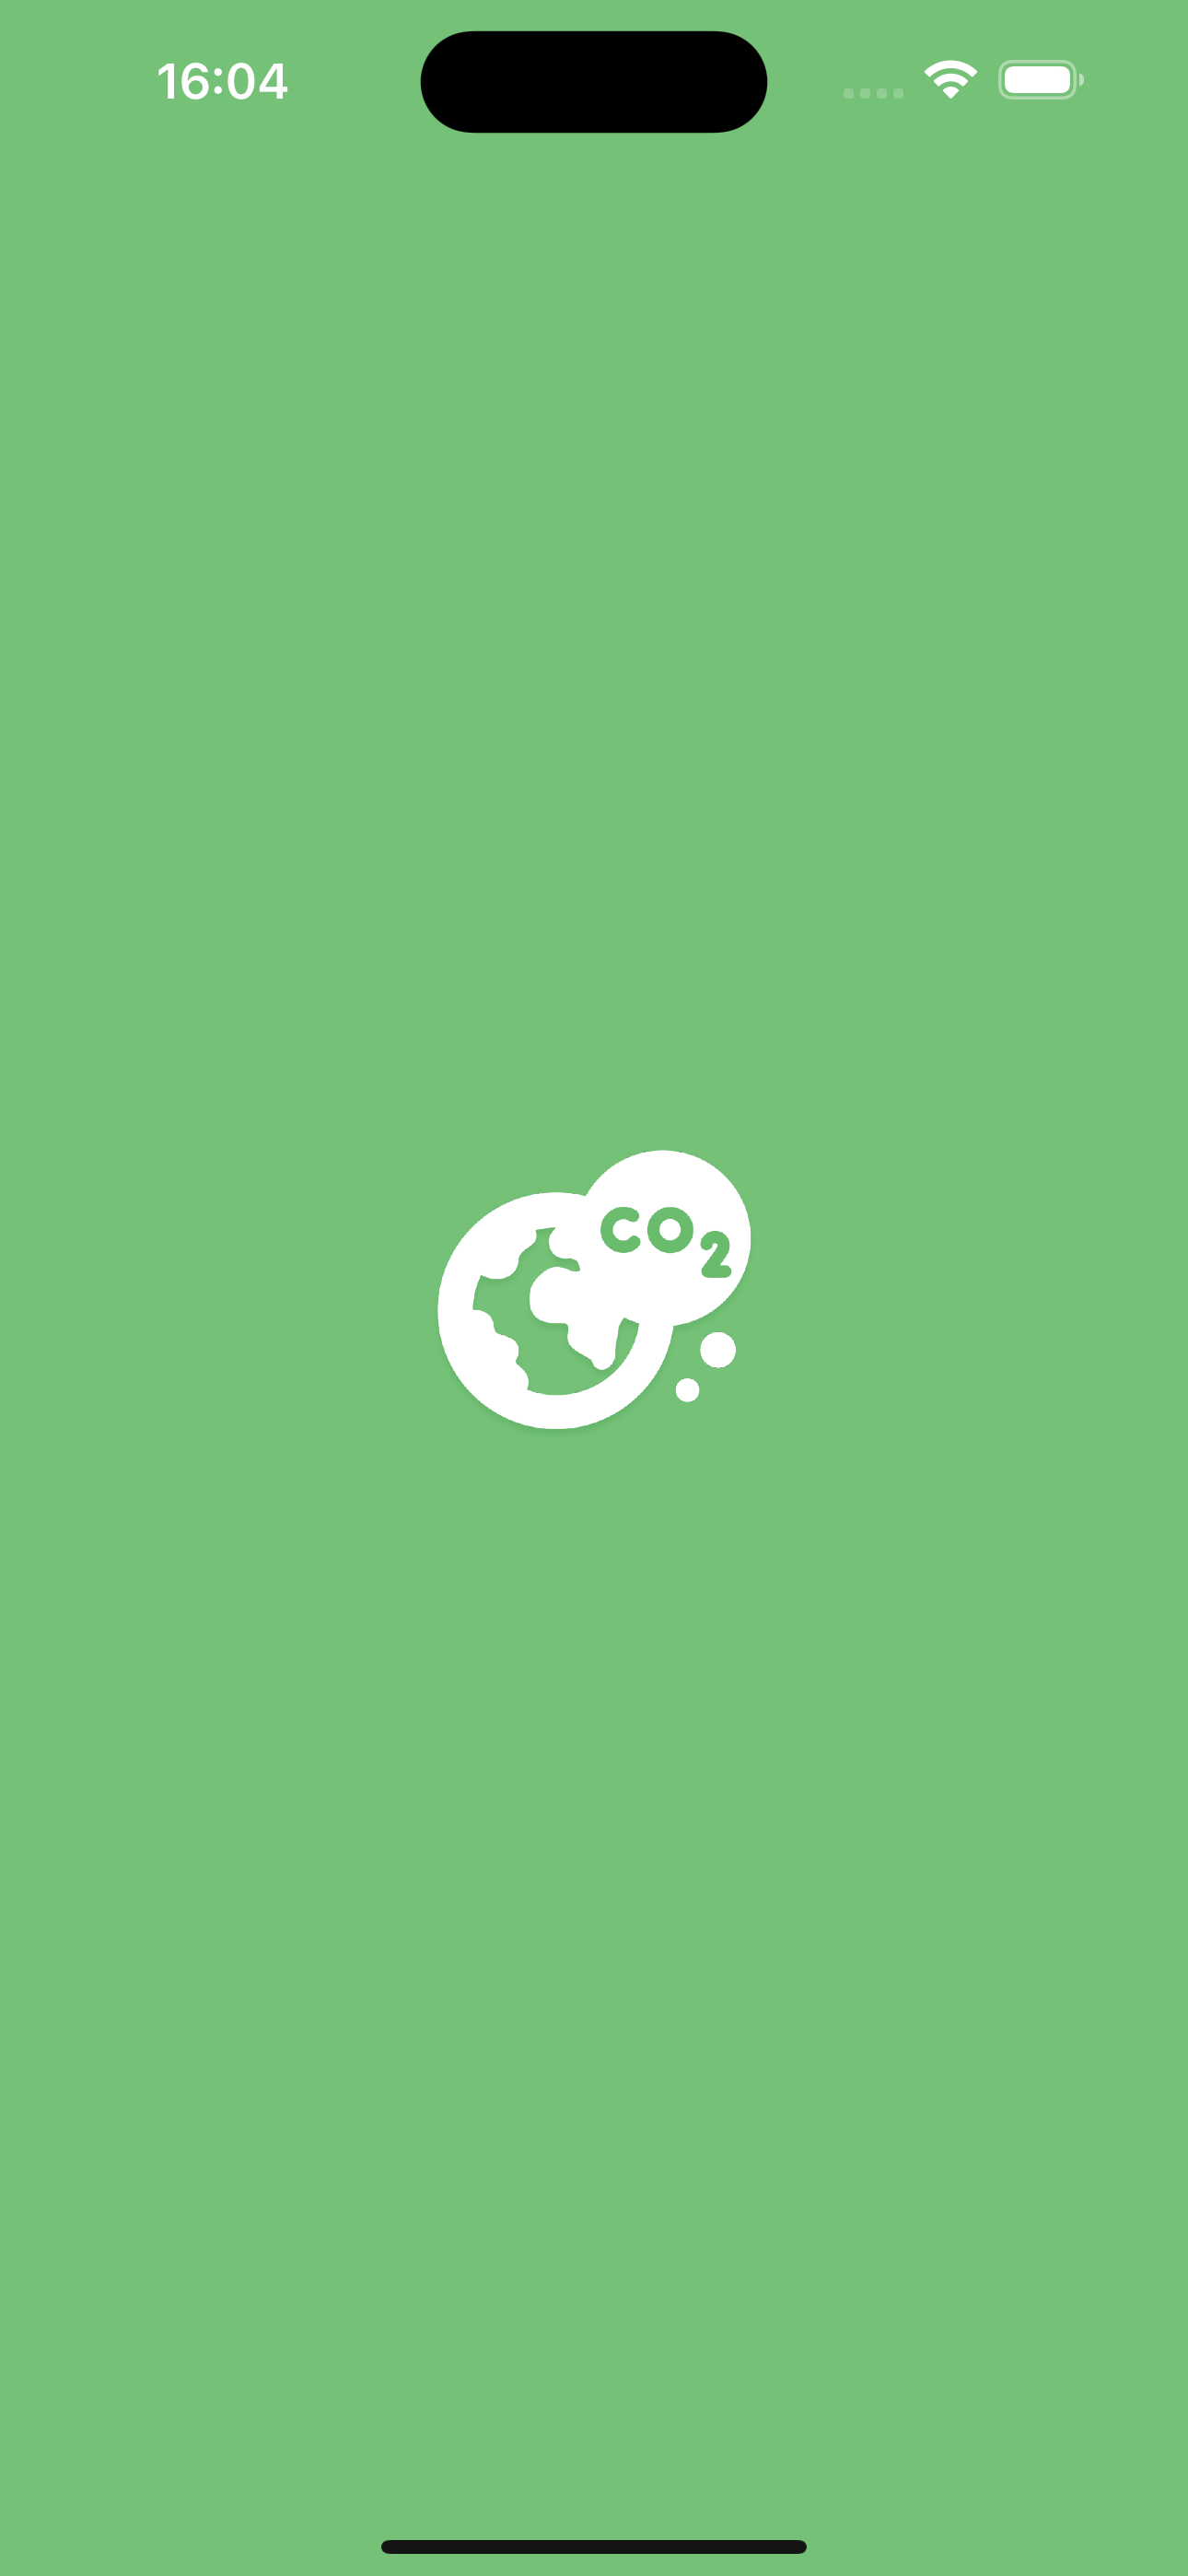
\includegraphics[width=0.45\textwidth]{Images/mobile/splash_screen.png}
  \caption[Màn hình chờ vào app]{\bfseries \fontsize{12pt}{0pt}
  \selectfont Màn hình chờ vào app}
  \label{splash_screen_waznet} %đặt tên cho ảnh
\end{figure}
\subsection{Các chức năng chung}
Tất cả các đối tượng sẽ có thể thực hiện được các chức năng chung sau:
\subsubsection{Chức năng đăng ký}
Người dùng sẽ phải nhập các thông tin và nhấn nút đăng ký. \textbf{Riêng với Admin} để đăng ký được cần có \textbf{một mã code} do bên nhà phát triển app cung cấp.

Một số lưu ý khi đăng ký:

\begin{adjustwidth}{1.5em}{}
  \begin{itemize}
    \item Họ và tên: phải điền một trong hai, không được để trống
    \item Số điện thoại: phải điền đúng format \textbf{10 số} (không kèm mã vùng)
    \item Mật khẩu: \textbf{đủ 8} ký tự trở lên
  \end{itemize}
\end{adjustwidth}
% \begin{figure}[H]
%   \centering
%   \includegraphics[width=12cm,height=3cm]{Images/mobile/}
%   \caption[Logo Firebase]{\bfseries \fontsize{12pt}{0pt}
%   \selectfont Logo Firebase}
%   \label{firebase_cover} %đặt tên cho ảnh
% \end{figure}
\begin{figure}[H]
  \centering
  \subcaptionbox{Màn đăng ký}{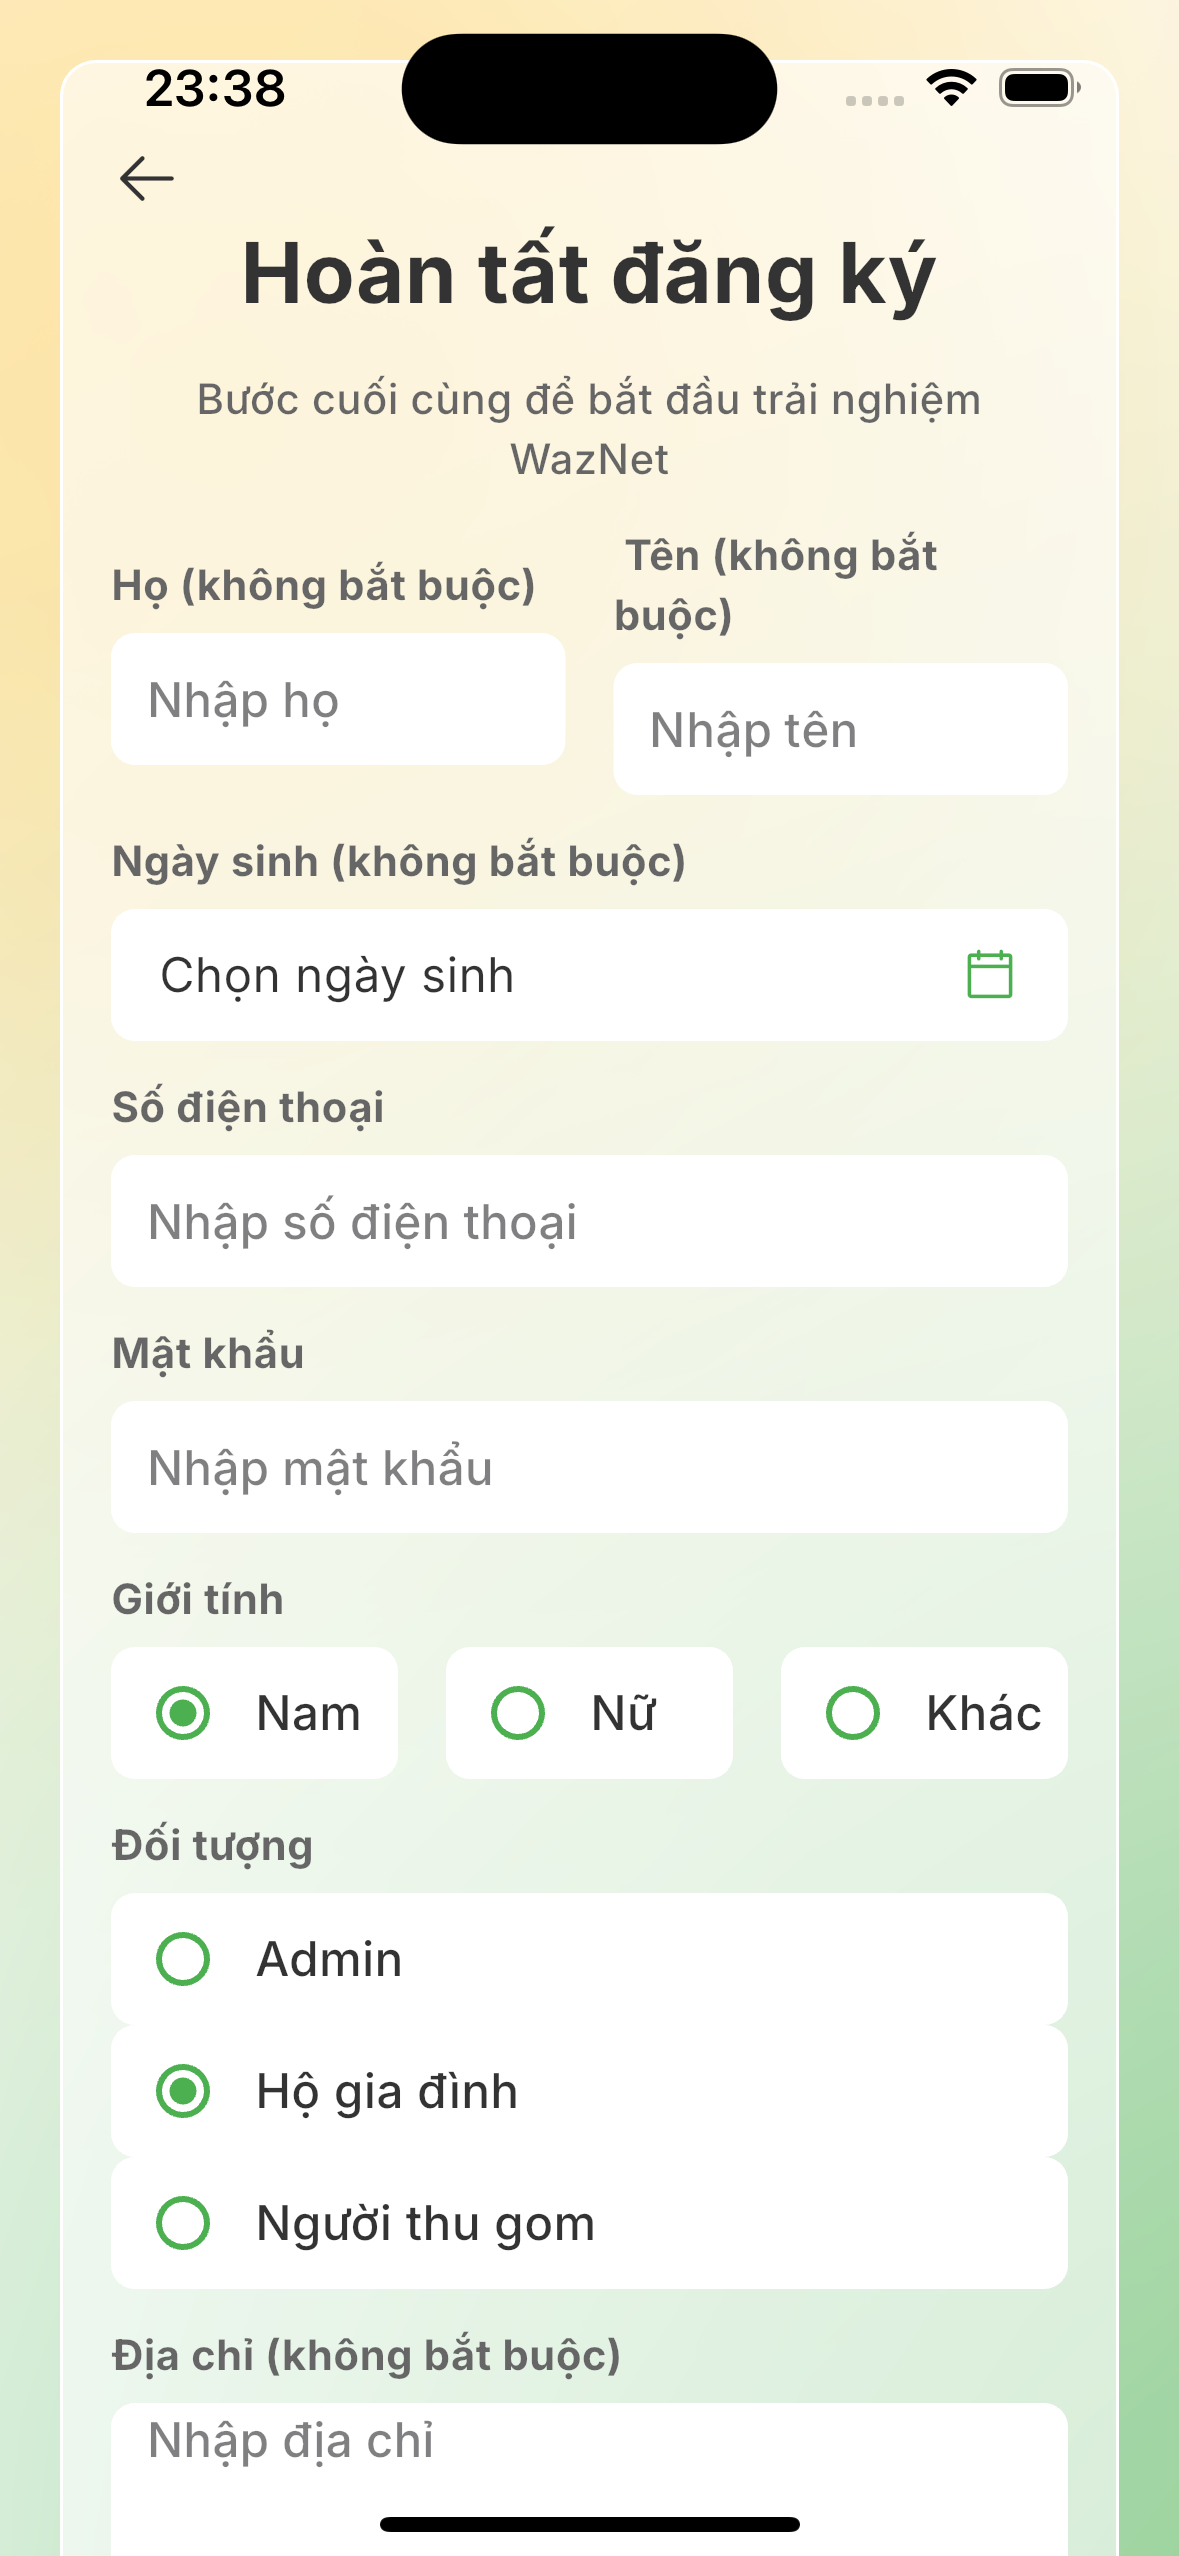
\includegraphics[width=0.45\textwidth]{Images/mobile/register_screen.png}}%
  \hfill
  \subcaptionbox{Màn đăng ký (tiếp)}{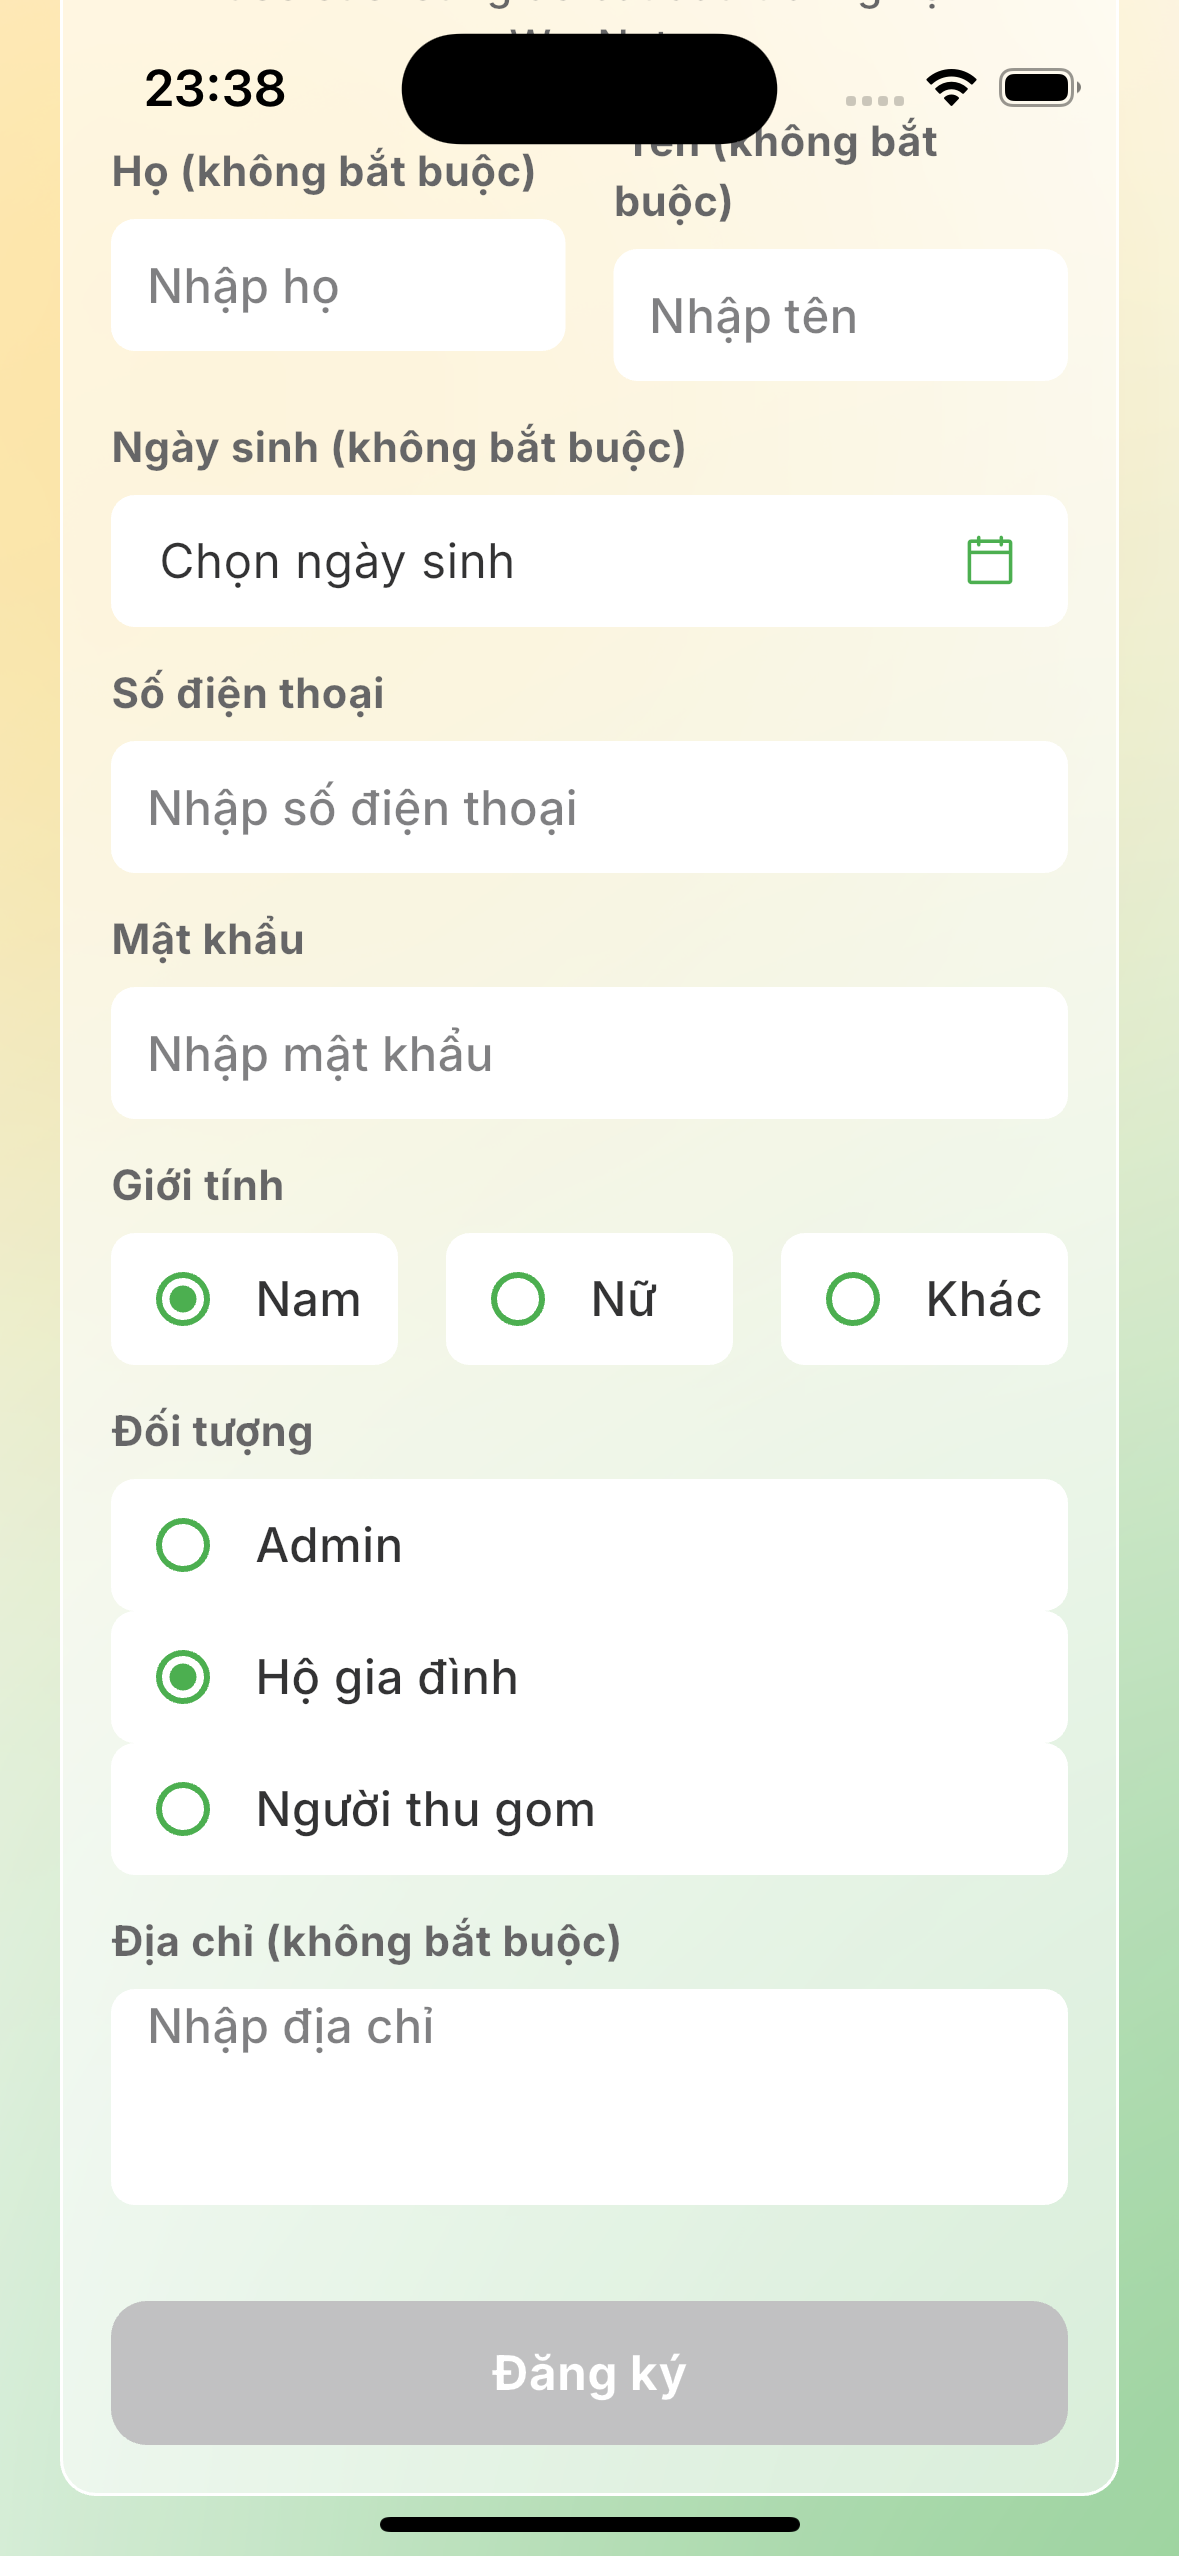
\includegraphics[width=0.45\textwidth]{Images/mobile/register_screen_2.png}}%
  \caption[Hình ảnh màn đăng ký]{\bfseries \fontsize{12pt}{0pt}
  \selectfont Hình ảnh màn đăng ký}
  \label{register_screen_waznet}
\end{figure}

% \begin{figure*}[ht!]
%   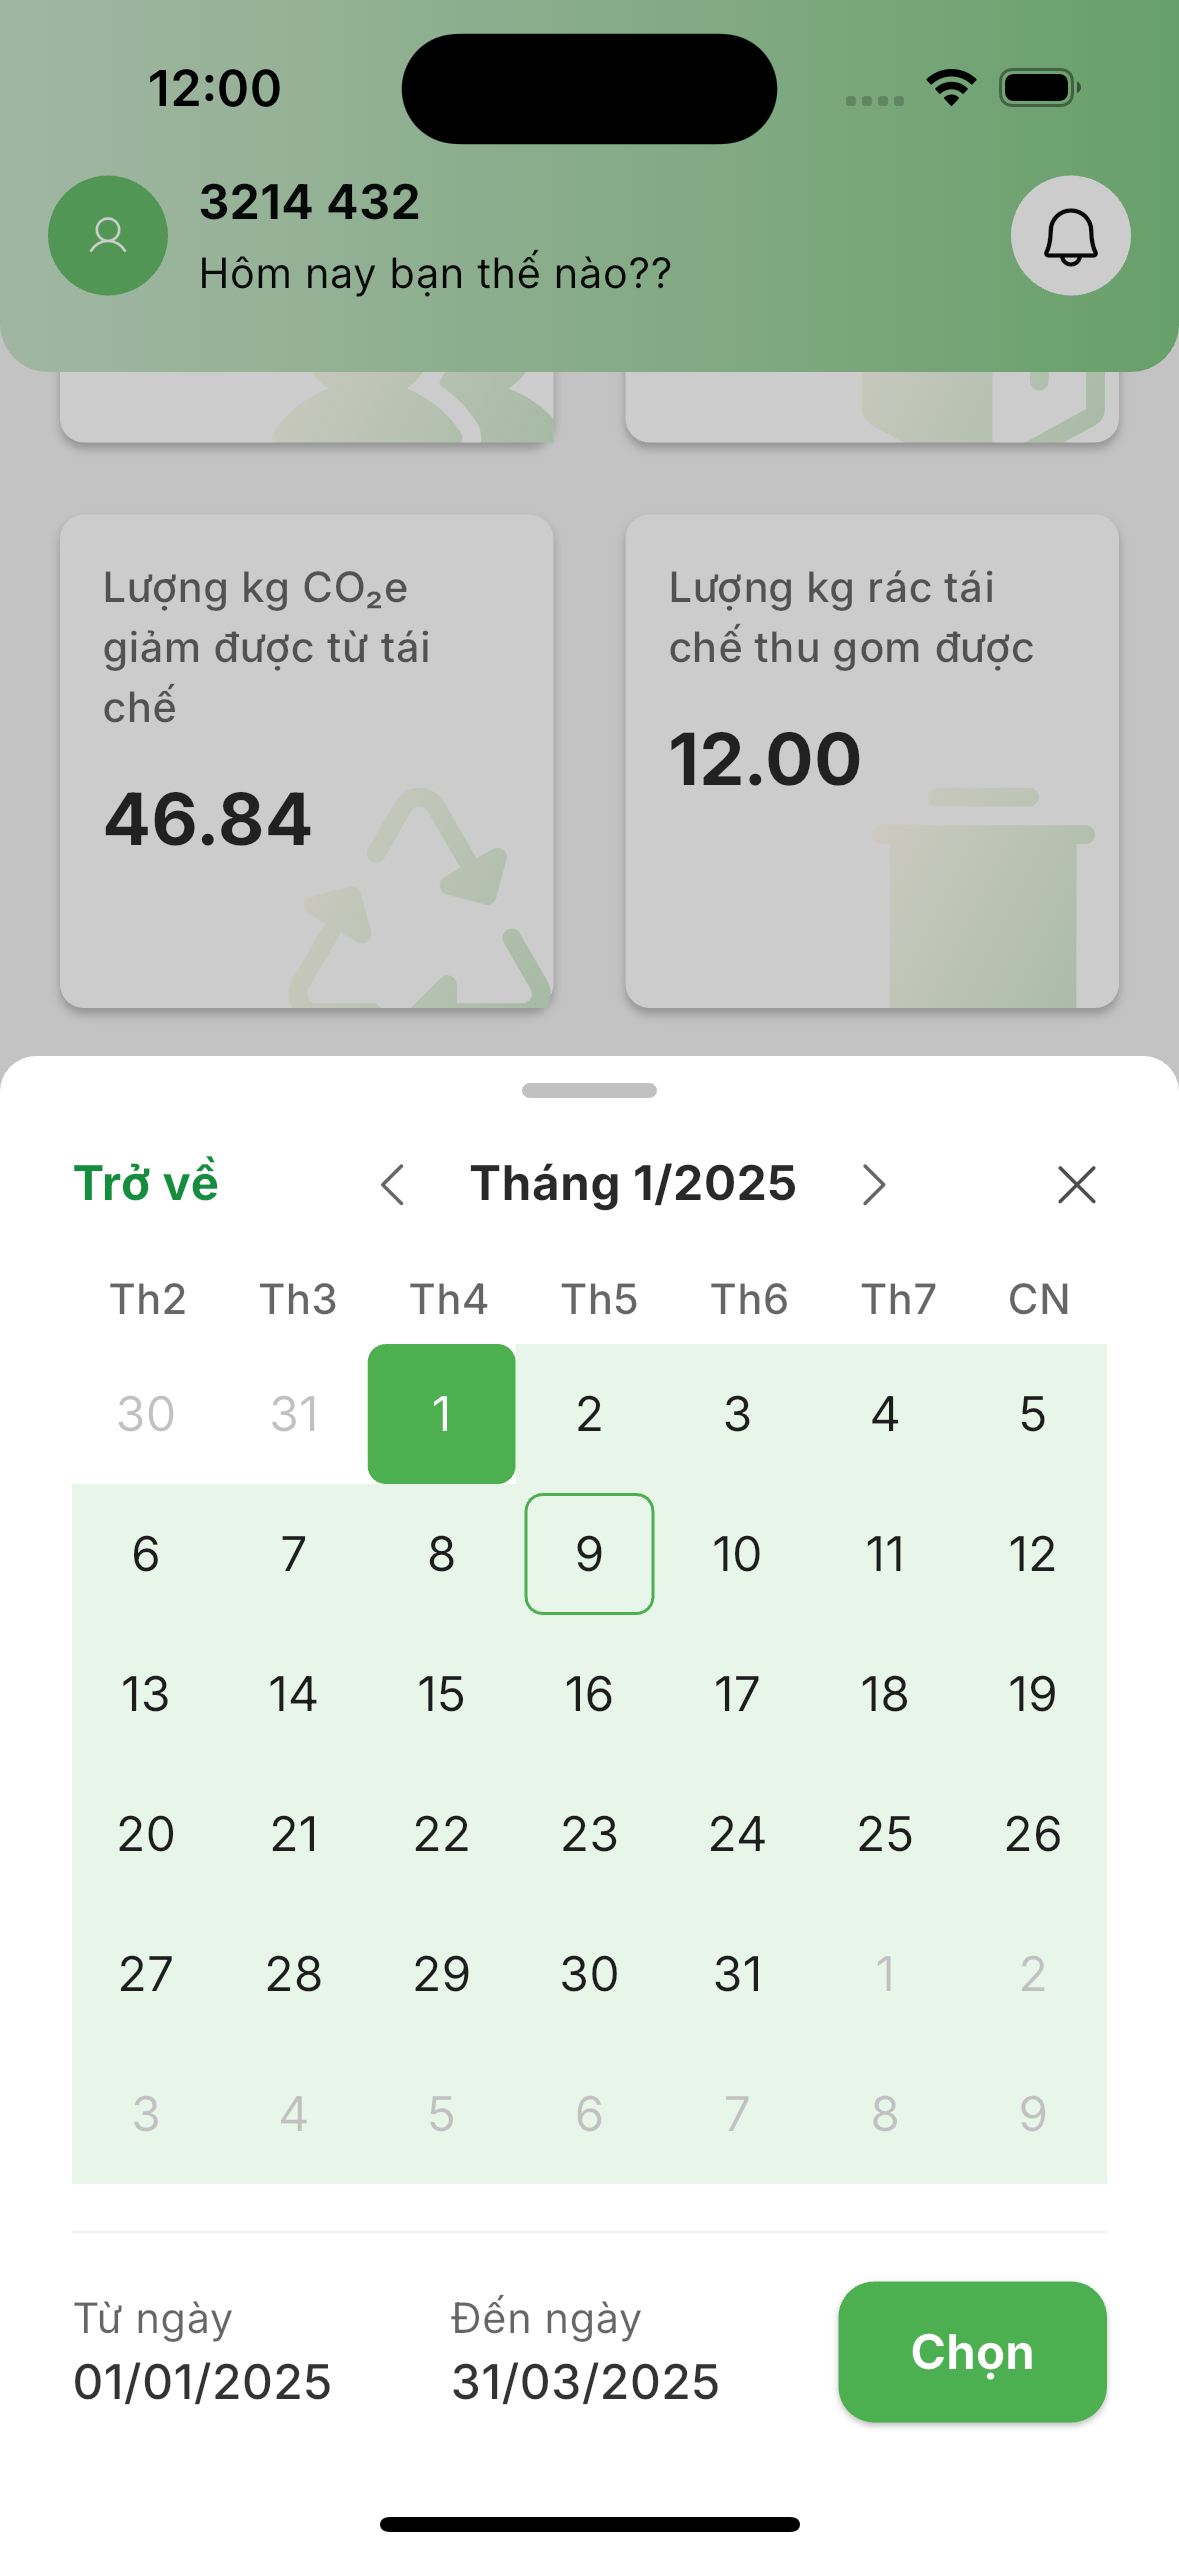
\includegraphics[width=.3\textwidth]{Images/mobile/filter_date.png}\hfill
%   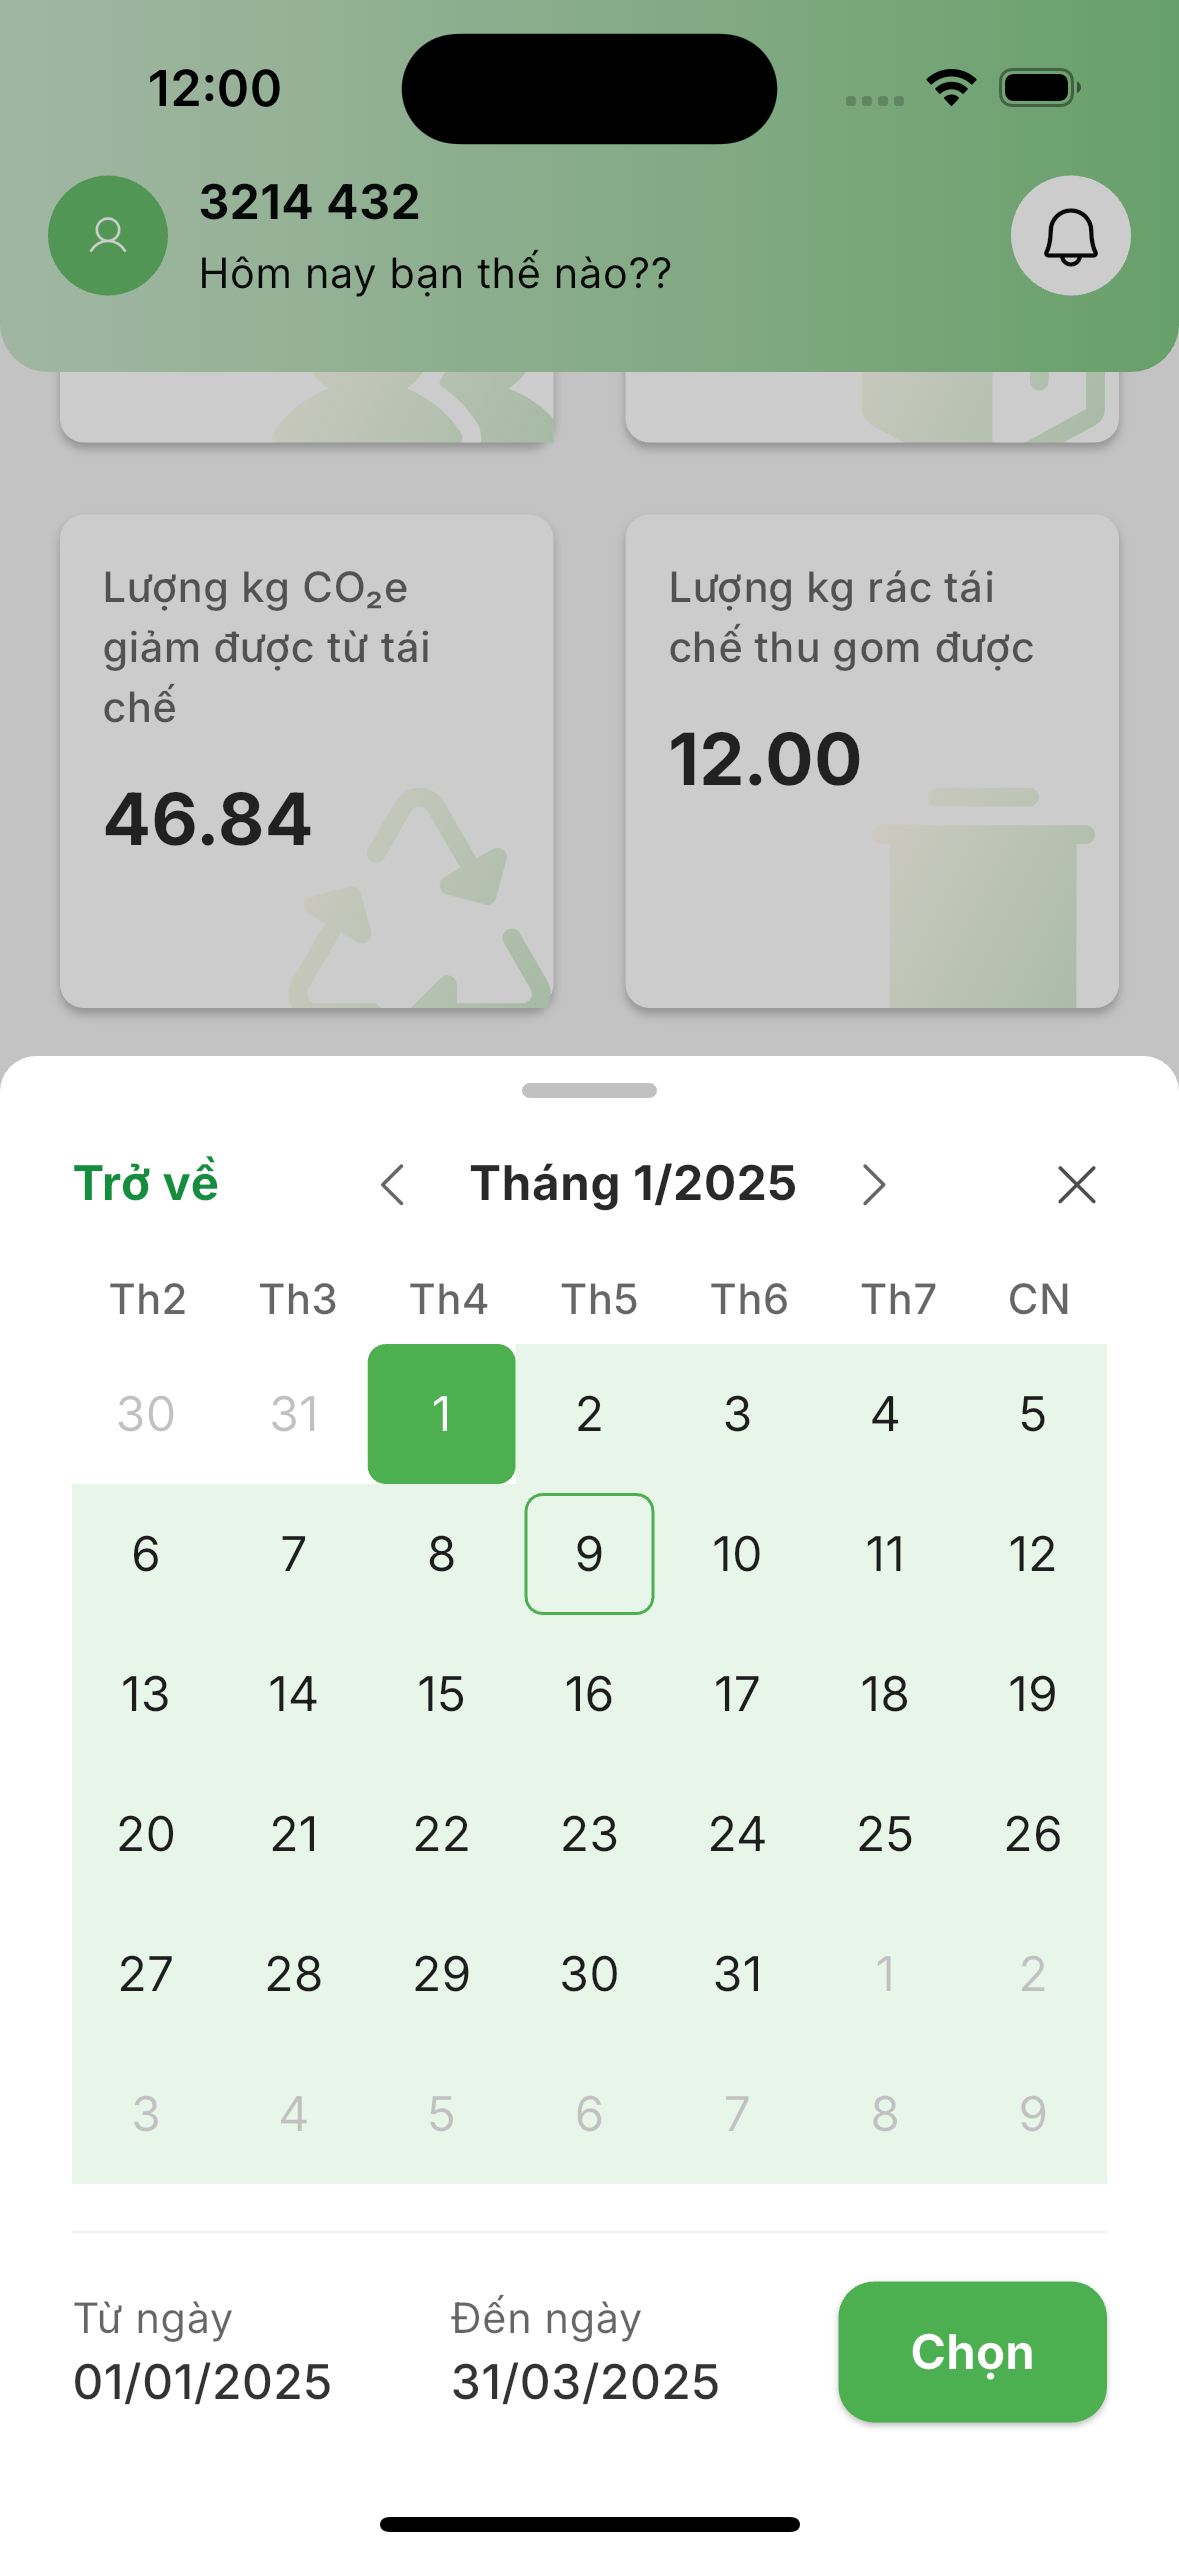
\includegraphics[width=.3\textwidth]{Images/mobile/filter_date.png}\hfill
%   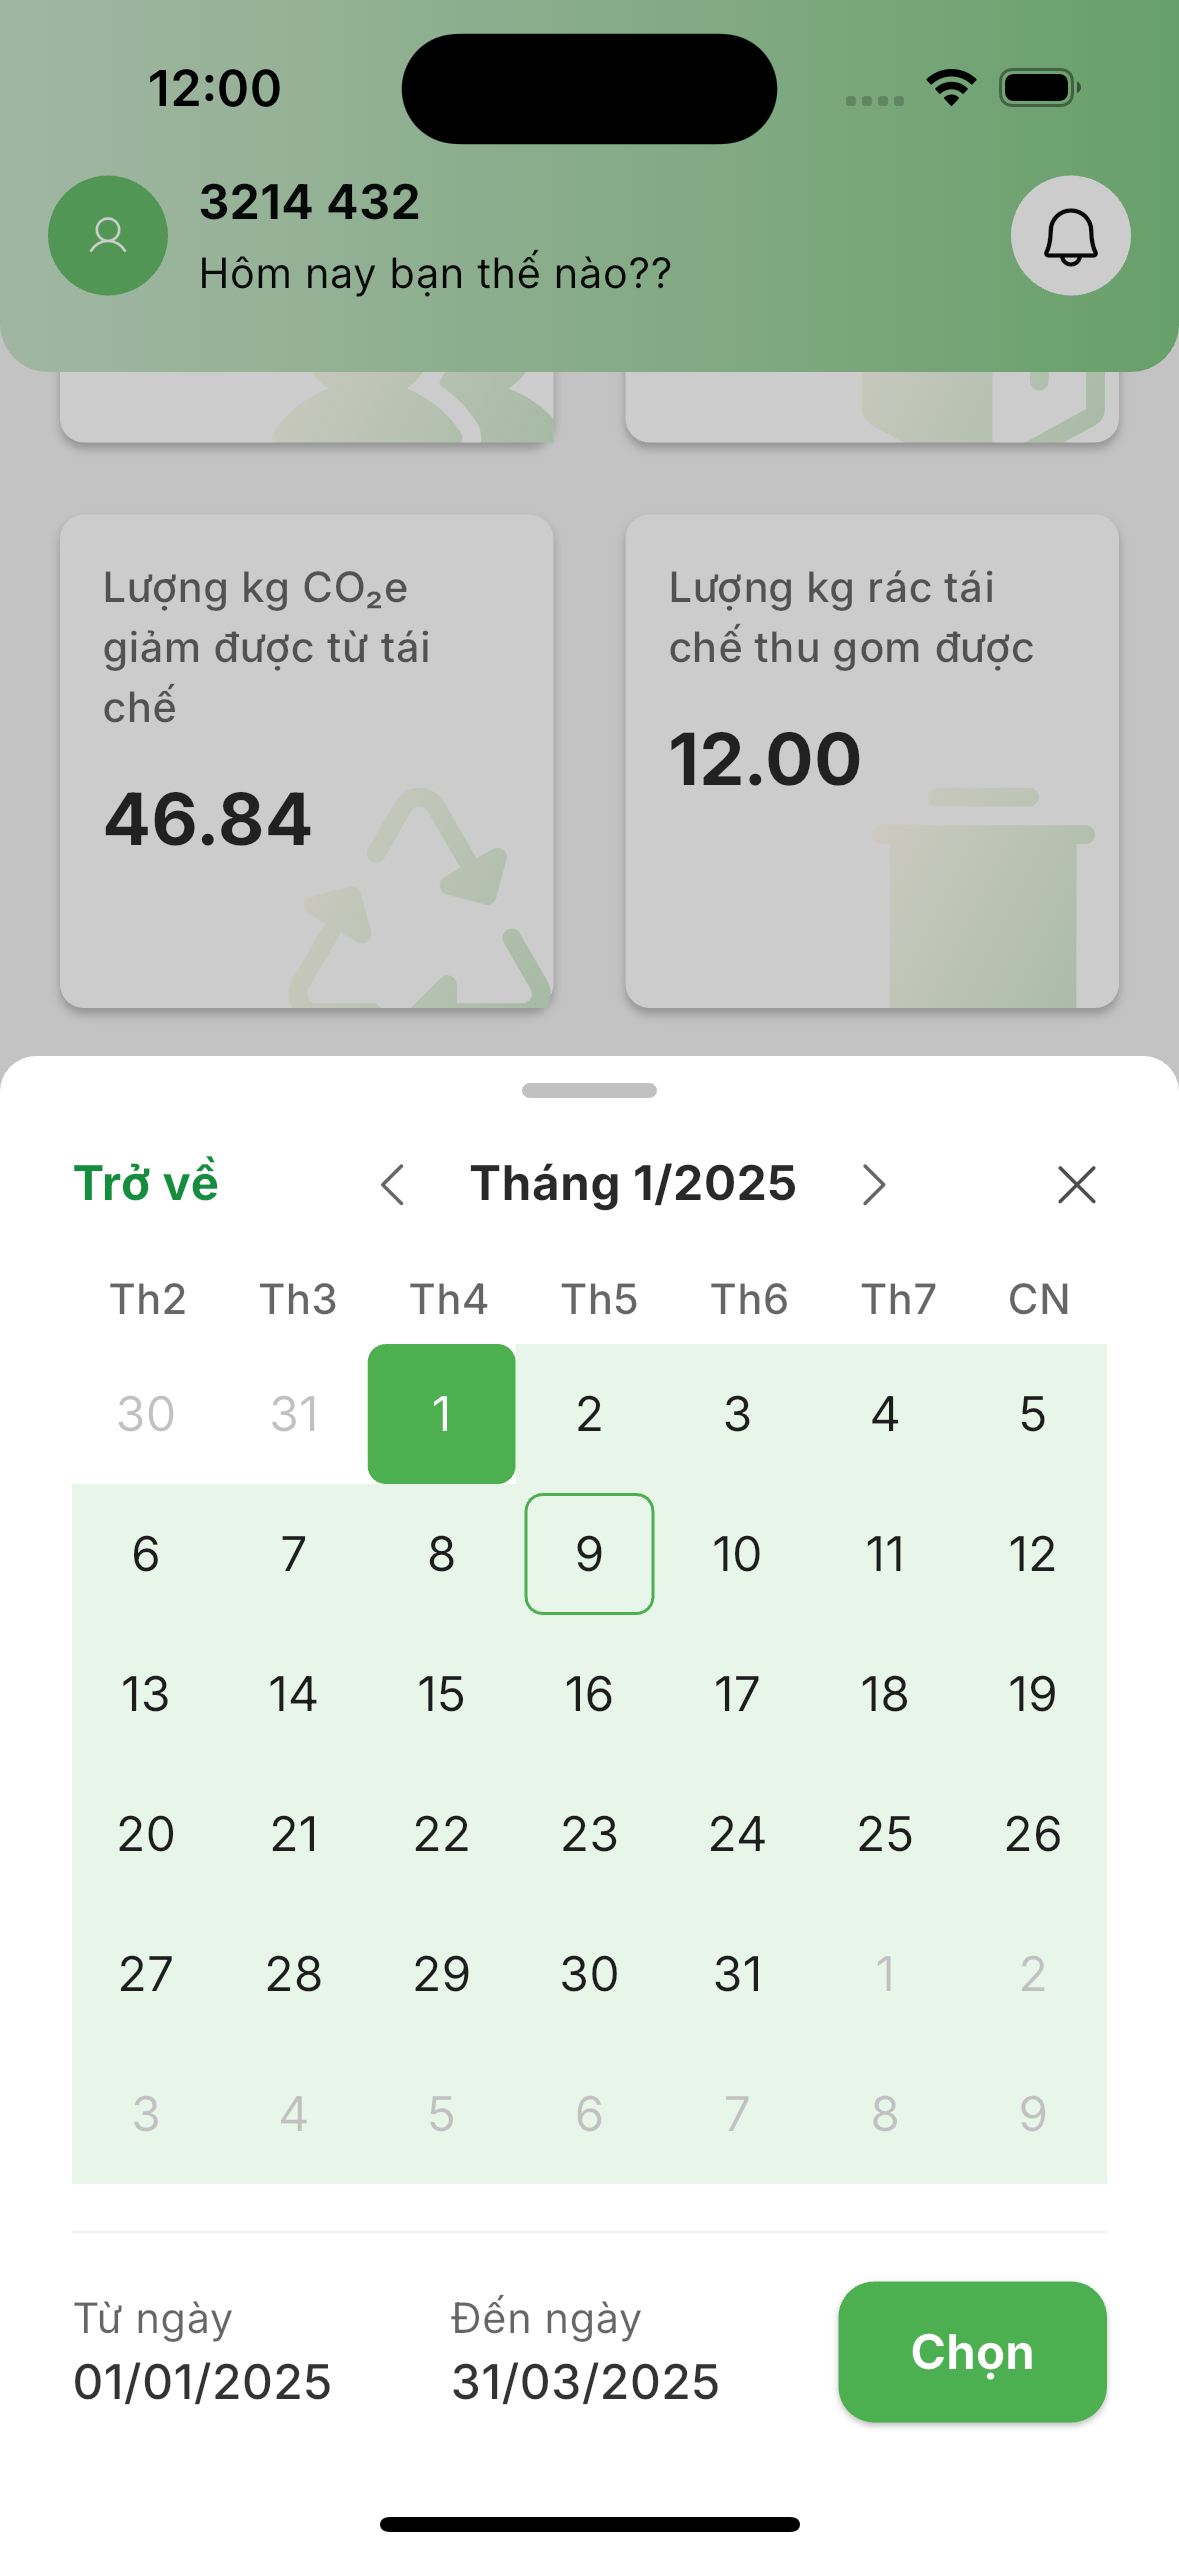
\includegraphics[width=.3\textwidth]{Images/mobile/filter_date.png}
%   \caption{Image A.}
%   \caption{Image B.}
%   \caption{Image C.}
% \end{figure*}

\subsubsection{Chức năng đăng nhập}
Người dùng sẽ phải nhập số điện thoại và mật khẩu để đăng nhập.
\begin{figure}[H]
  \centering
  \subcaptionbox{Màn nhập số điện thoại}{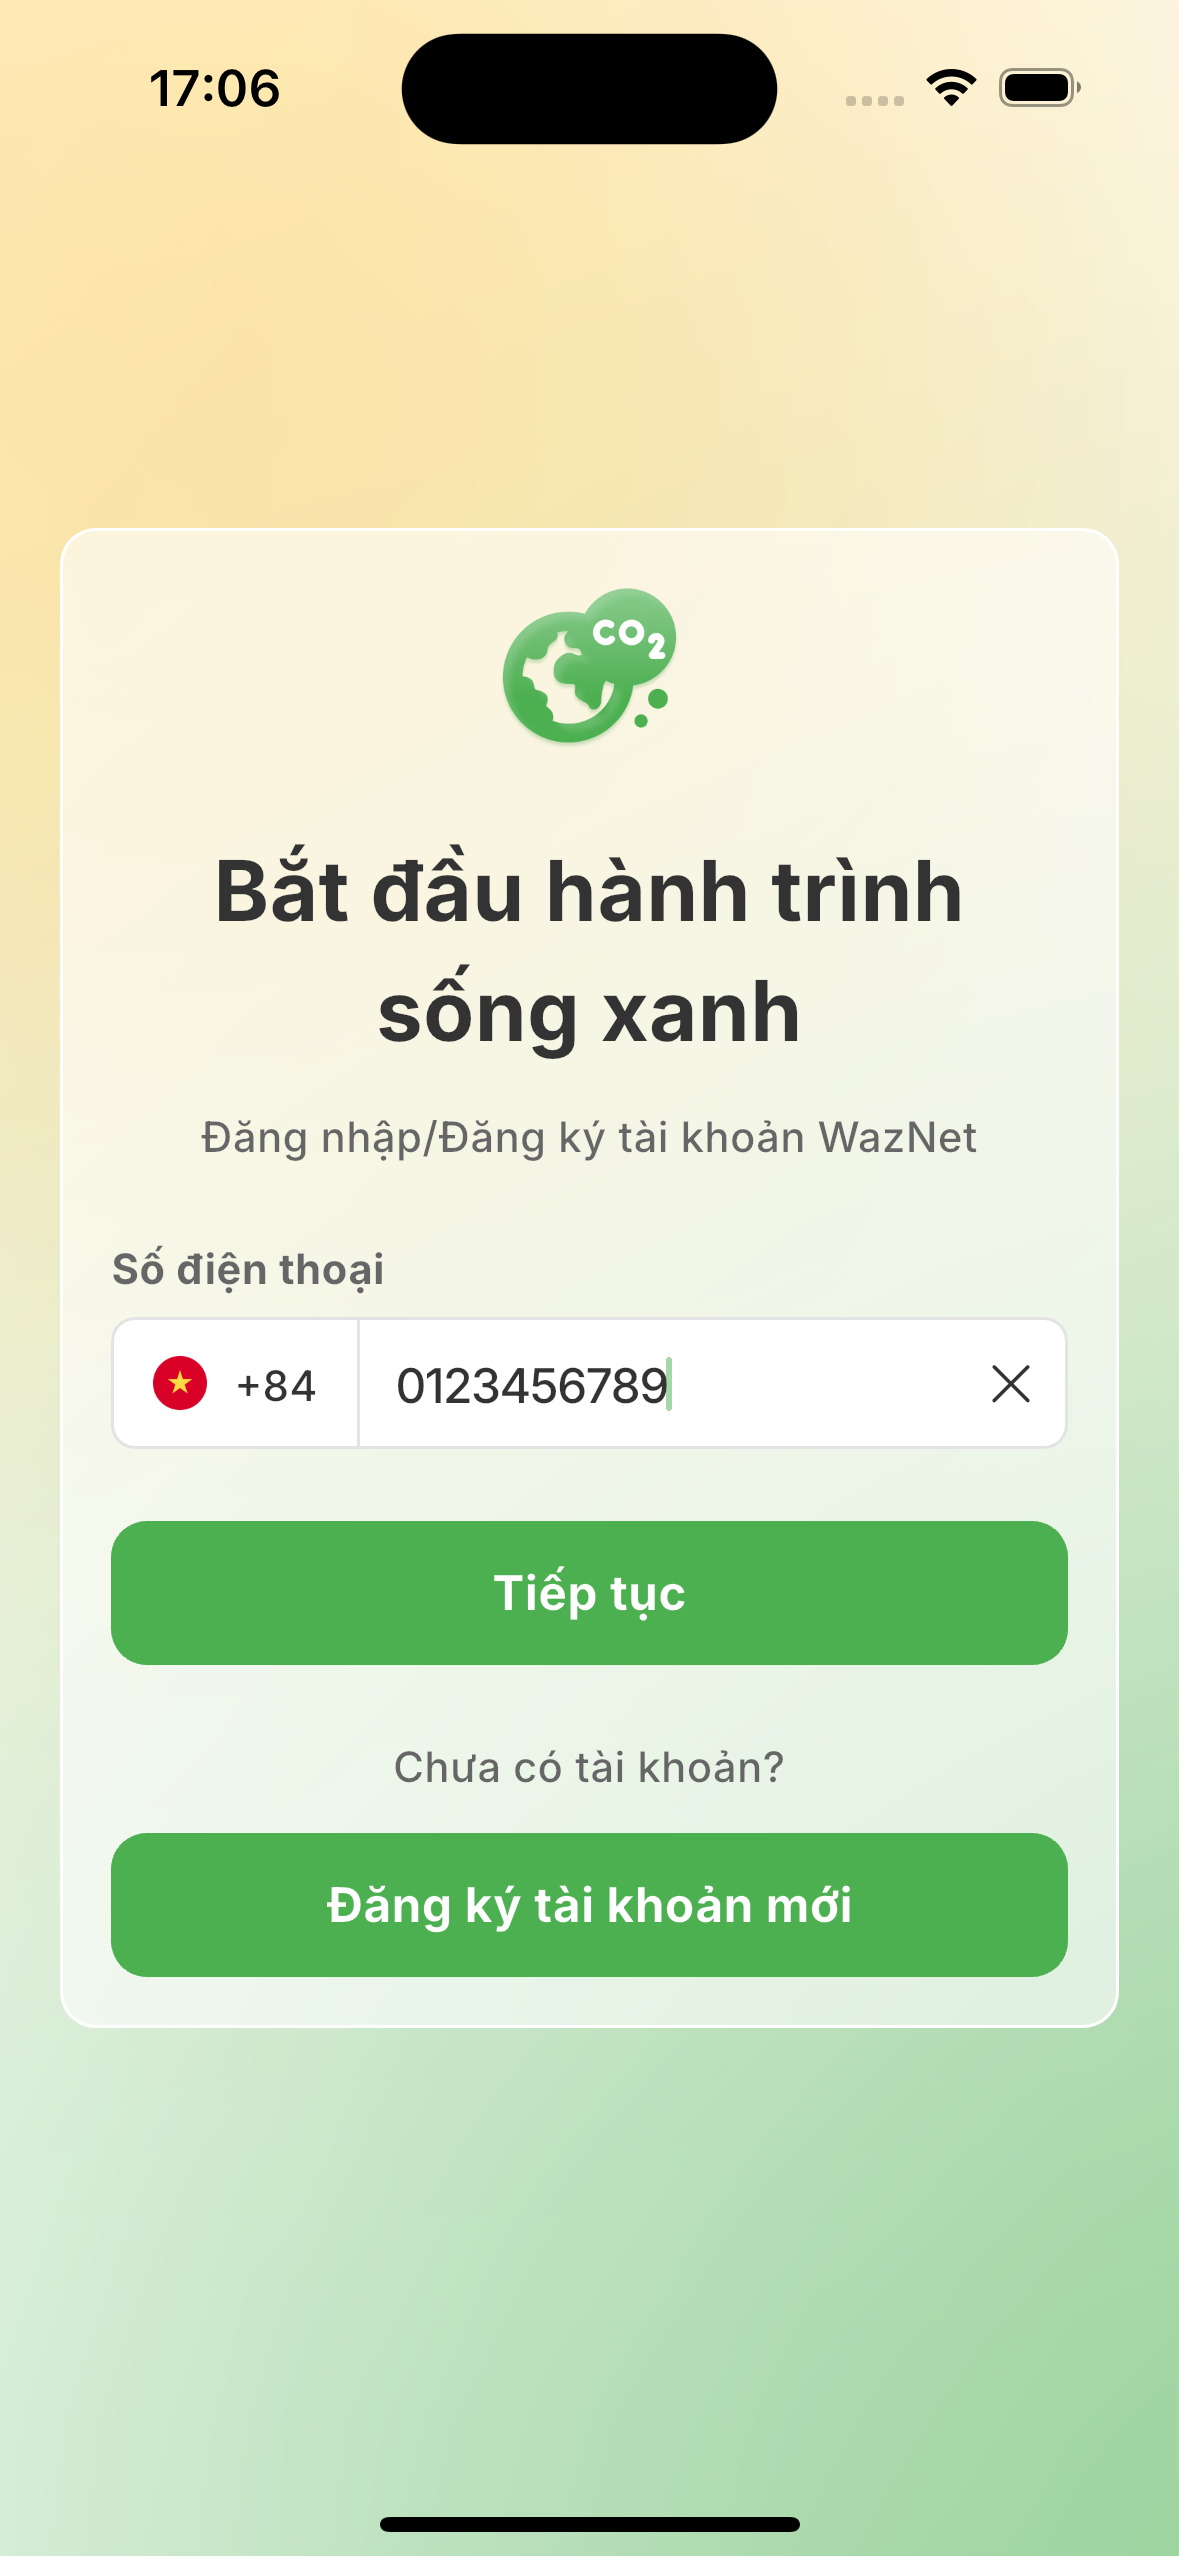
\includegraphics[width=0.32\textwidth]{Images/mobile/login_screen_1.png}}%
  \hfill
  \subcaptionbox{Màn nhập mật khẩu (lỗi)}{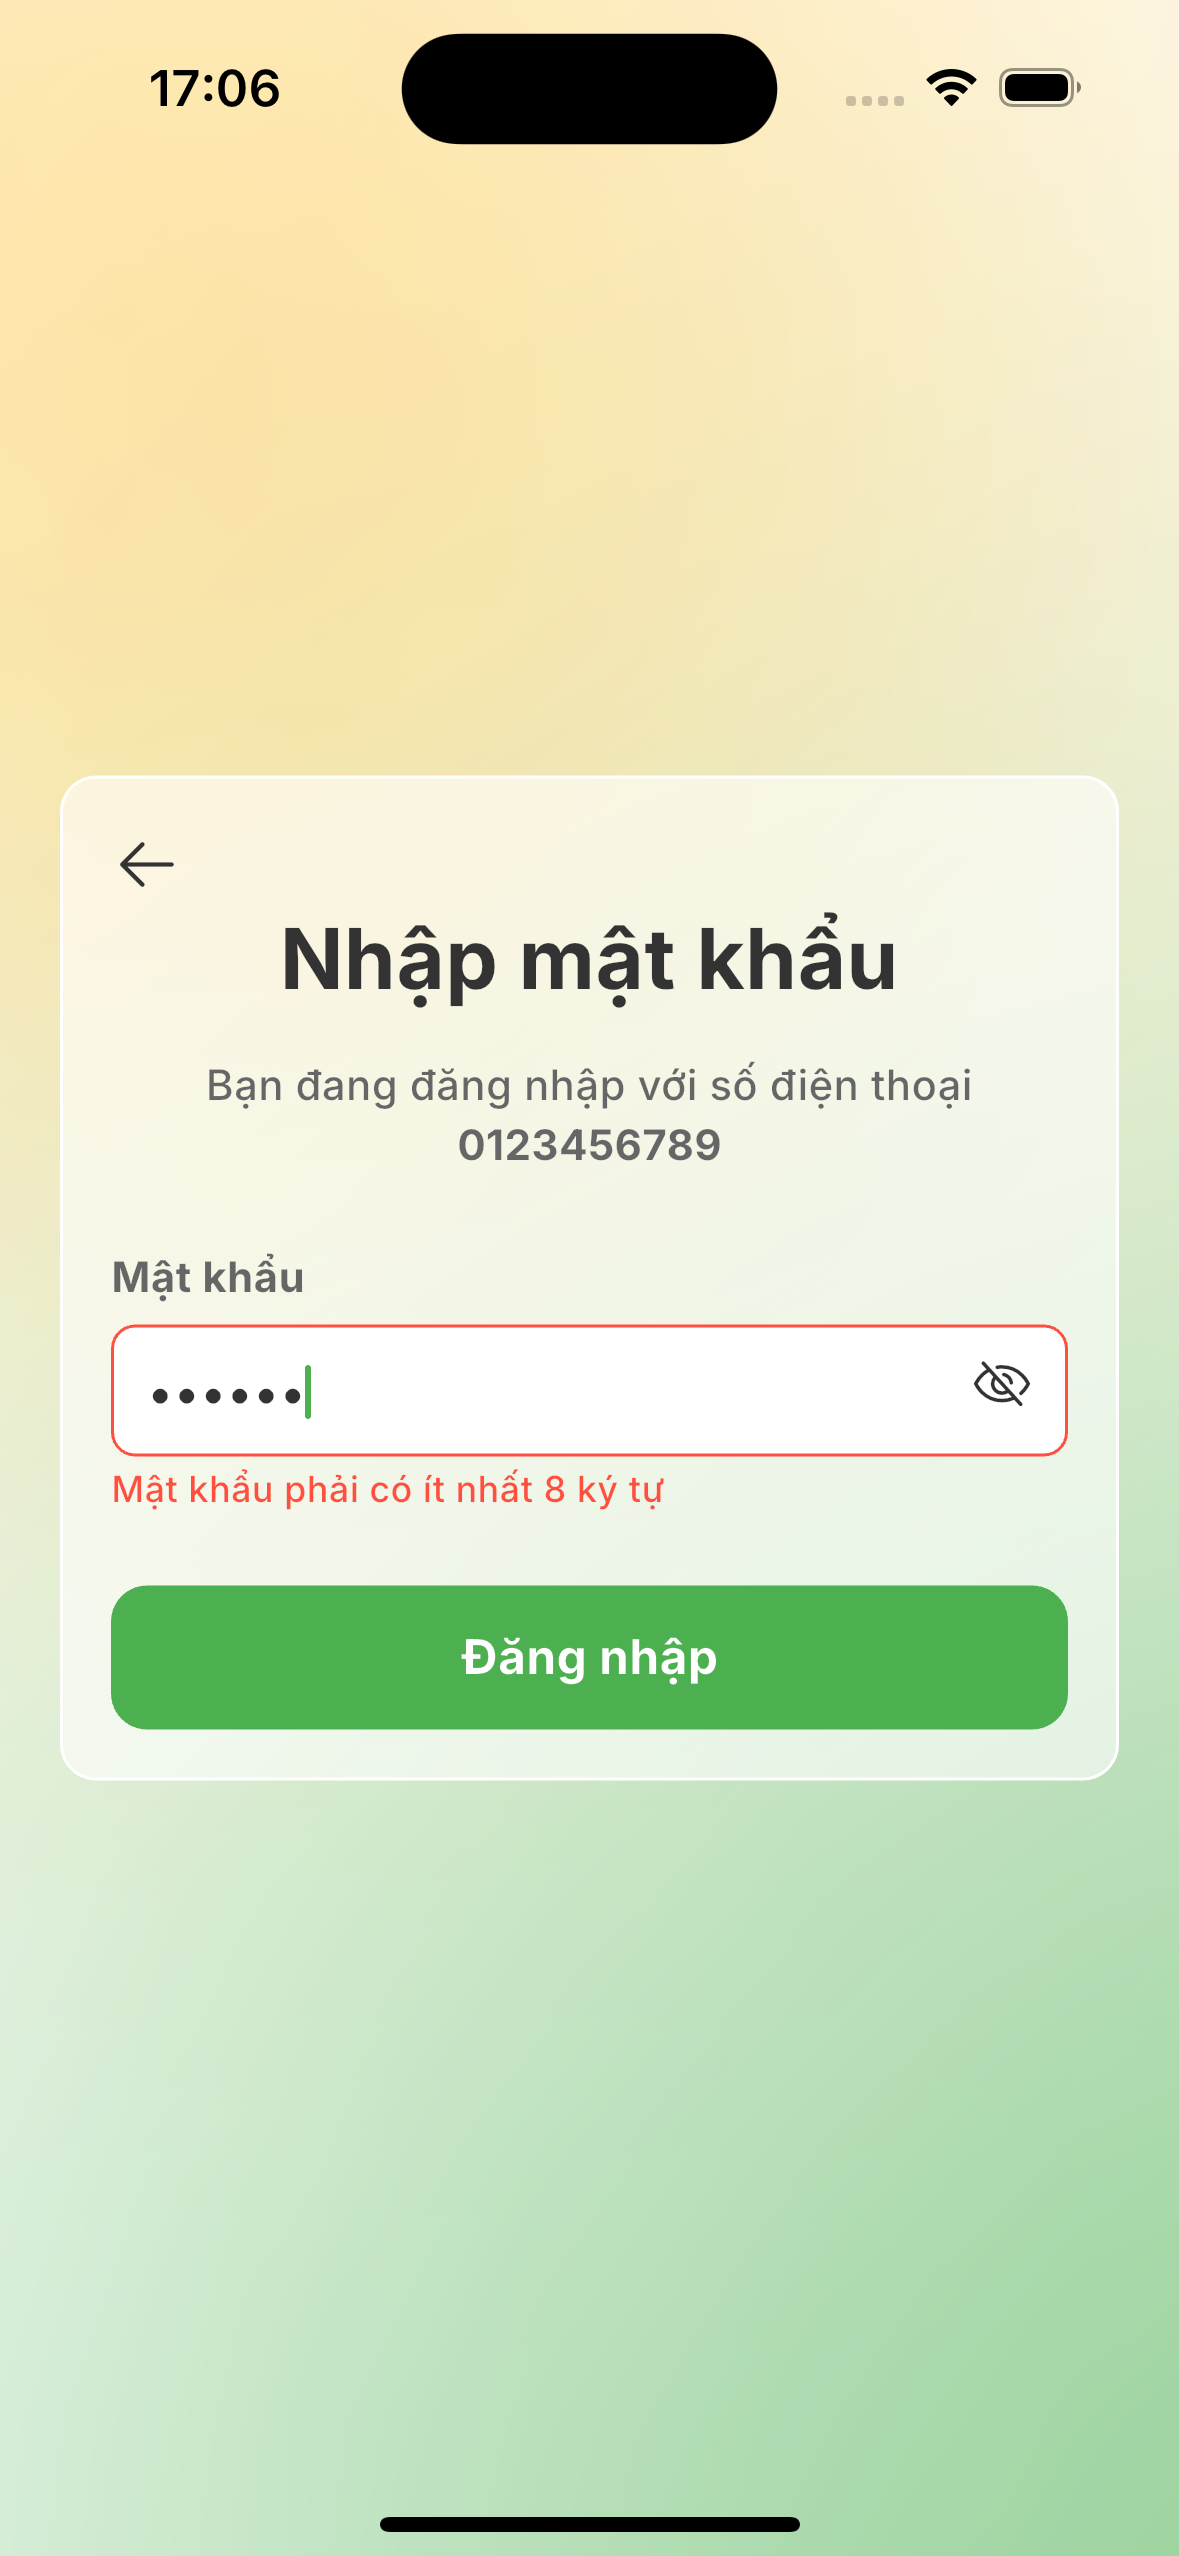
\includegraphics[width=0.32\textwidth]{Images/mobile/login_screen_2.png}}%
  \hfill
  \subcaptionbox{Màn đăng nhập (đủ ký tự)}{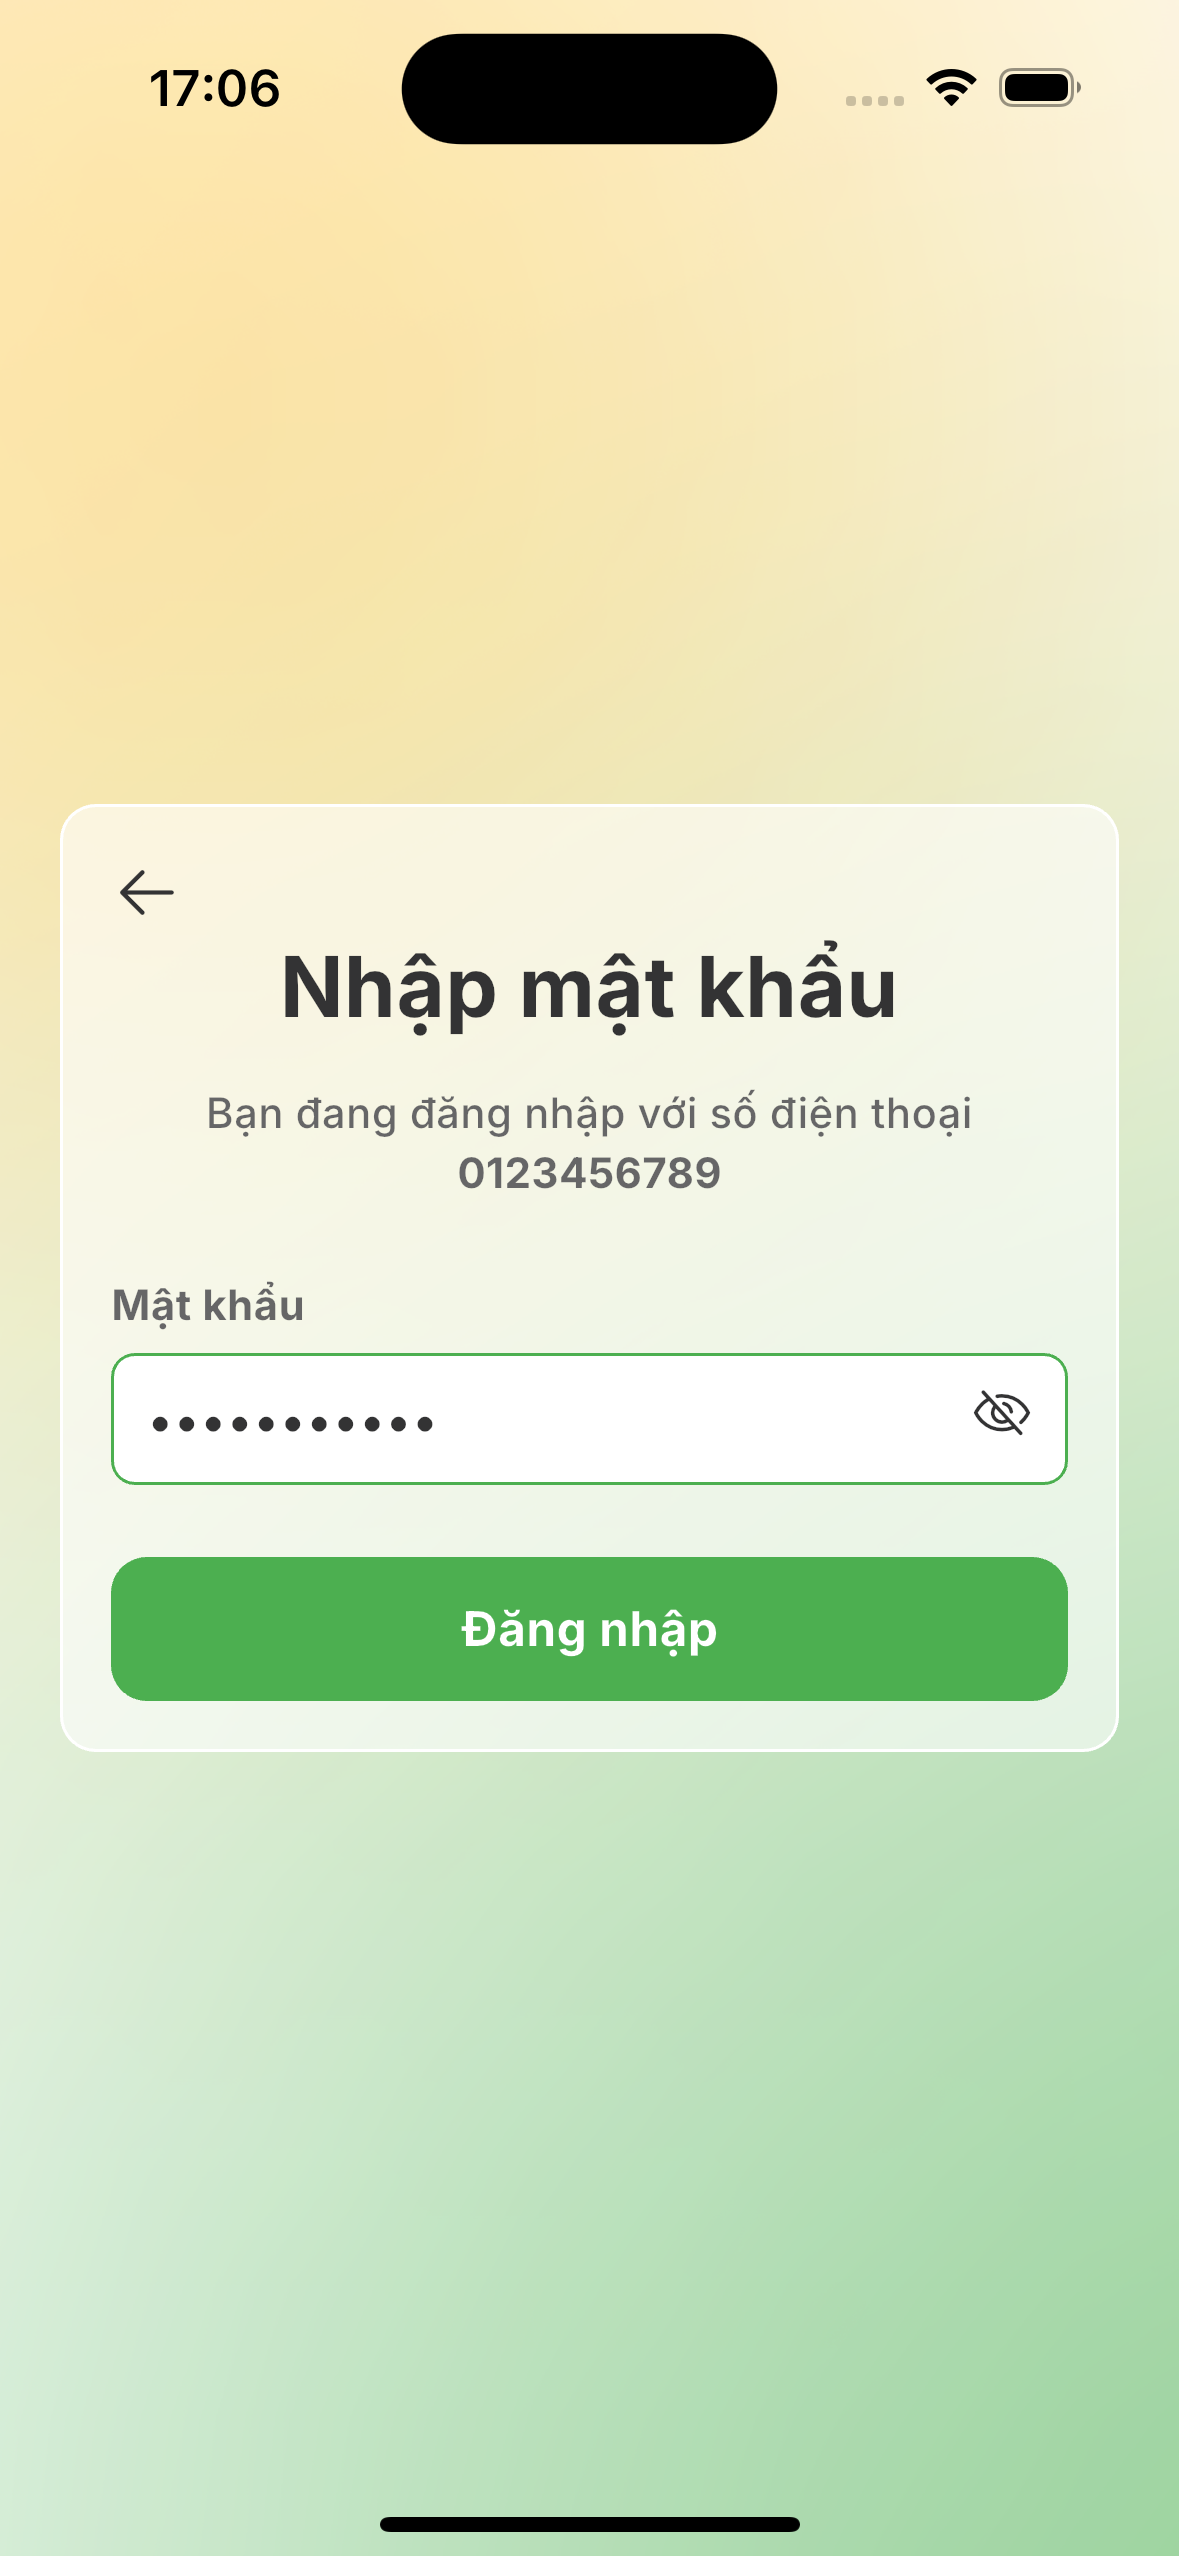
\includegraphics[width=0.32\textwidth]{Images/mobile/login_screen_3.png}}%
  \caption[Hình ảnh màn đăng nhập]{\bfseries \fontsize{12pt}{0pt}
  \selectfont Hình ảnh màn đăng nhập}
  \label{login_screen_waznet}
\end{figure}

\subsubsection{Chức năng xem chi tiết đóng góp đã nhập theo ngày}
Đối với Hộ gia đình và người thu gom, nhấn vào tab \textbf{Số liệu}, chọn một ngày, dữ liệu sẽ hiển thị như hình dưới
\begin{figure}[H]
  \centering
  \subcaptionbox{Màn danh sách đóng góp}{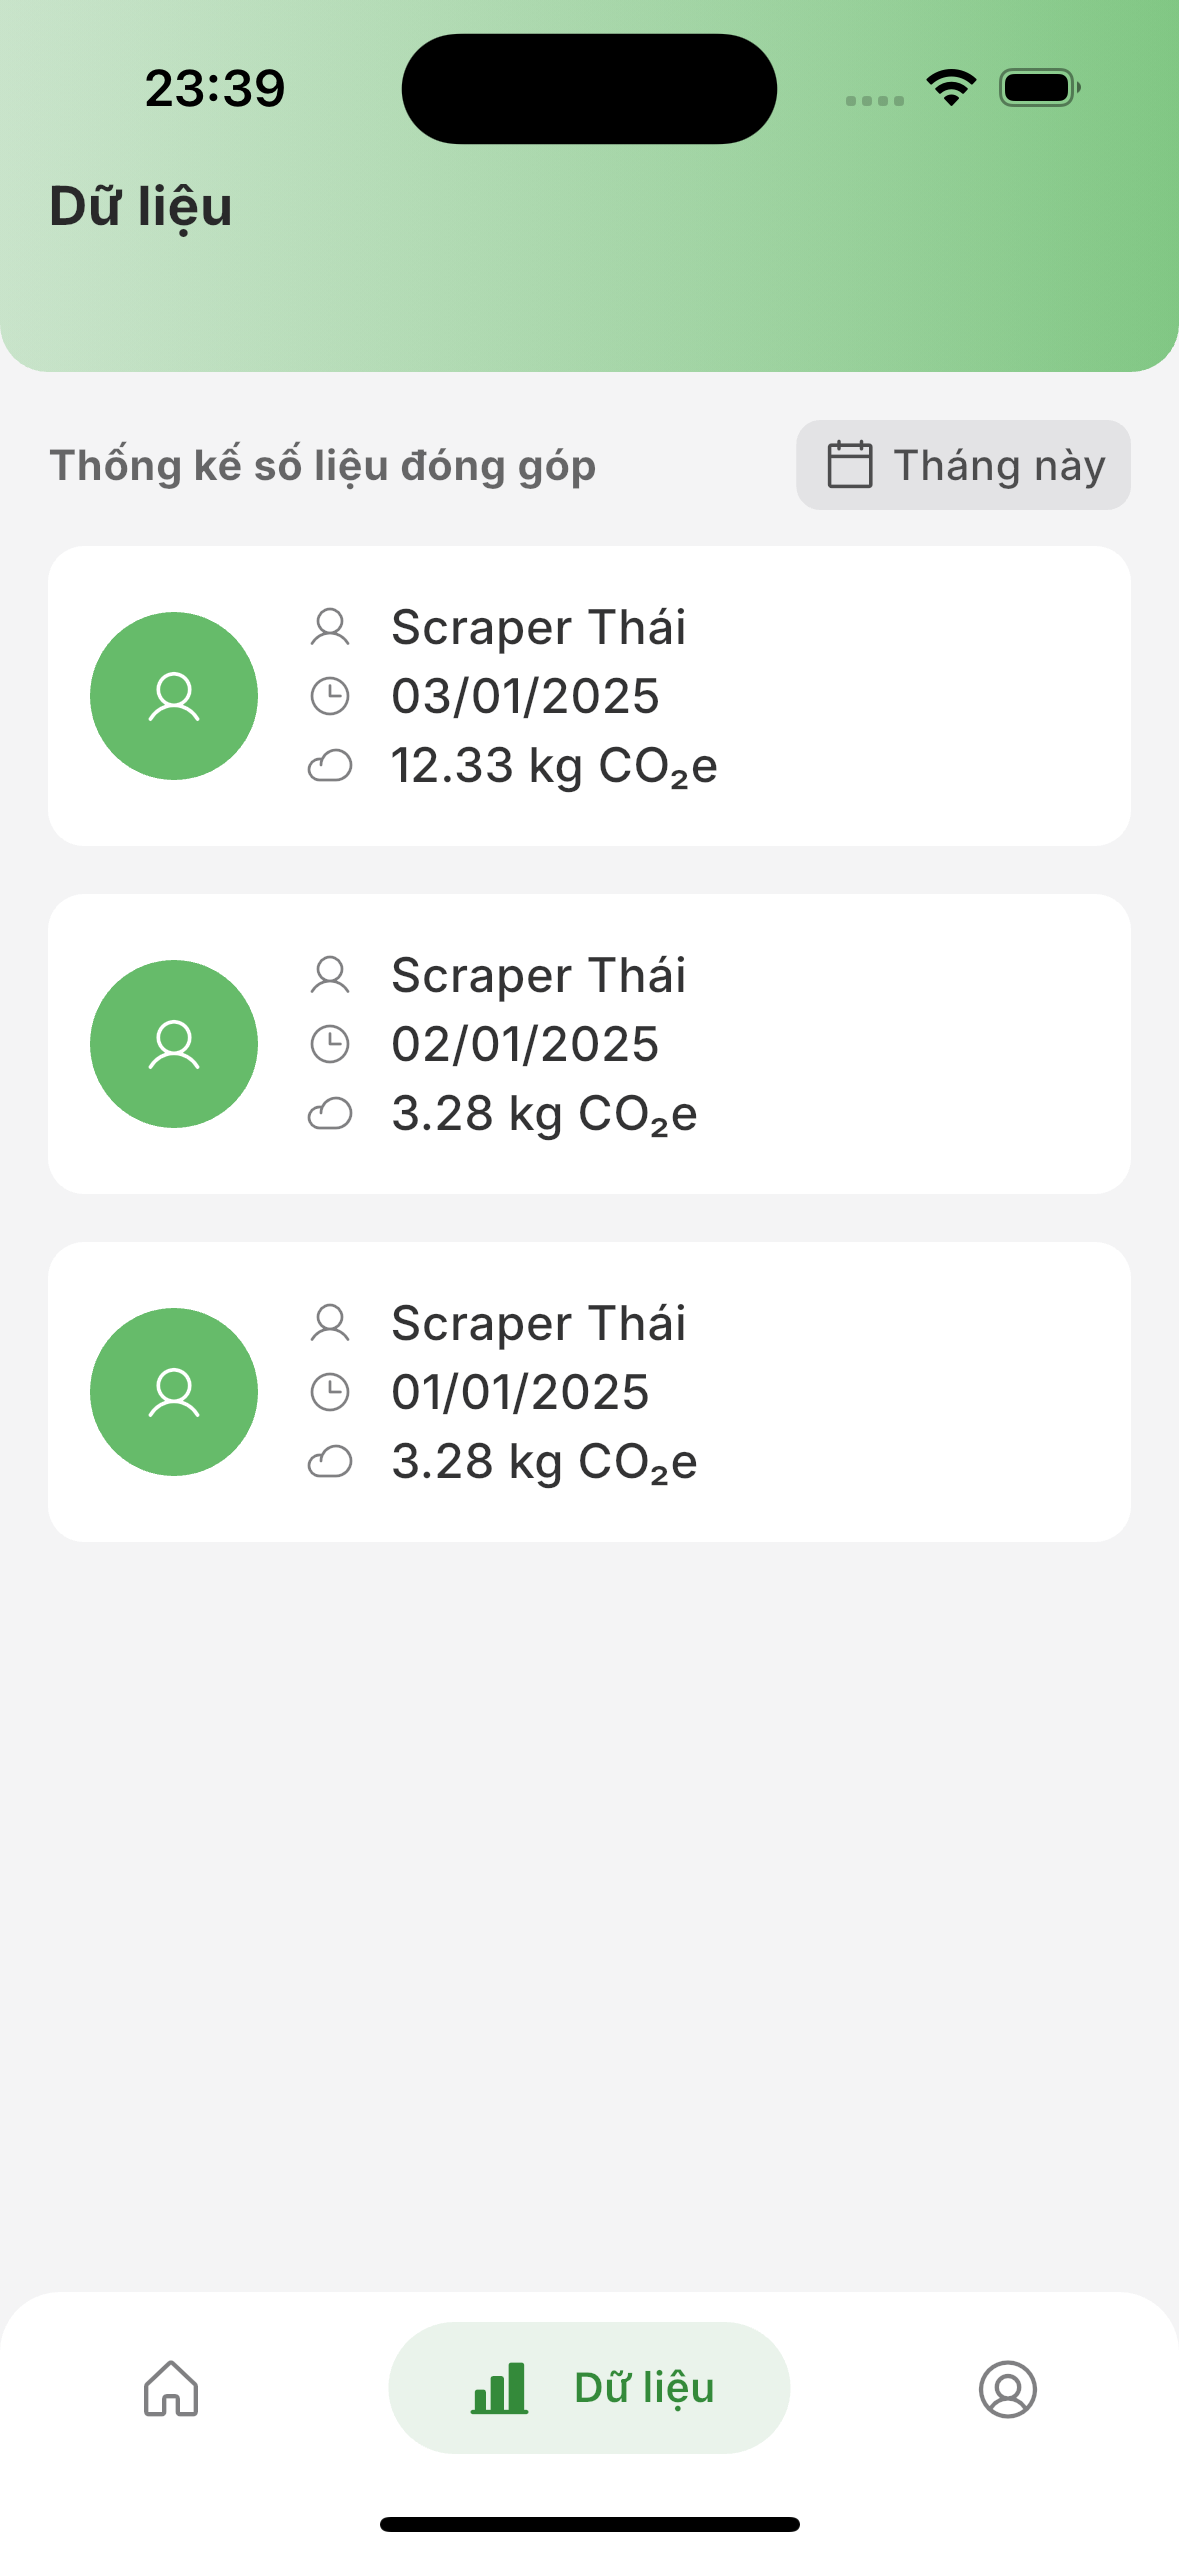
\includegraphics[width=0.45\textwidth]{Images/mobile/contributions_screen.png}}%
  \hfill
  \subcaptionbox{Màn chi tiết đóng góp trong một ngày}{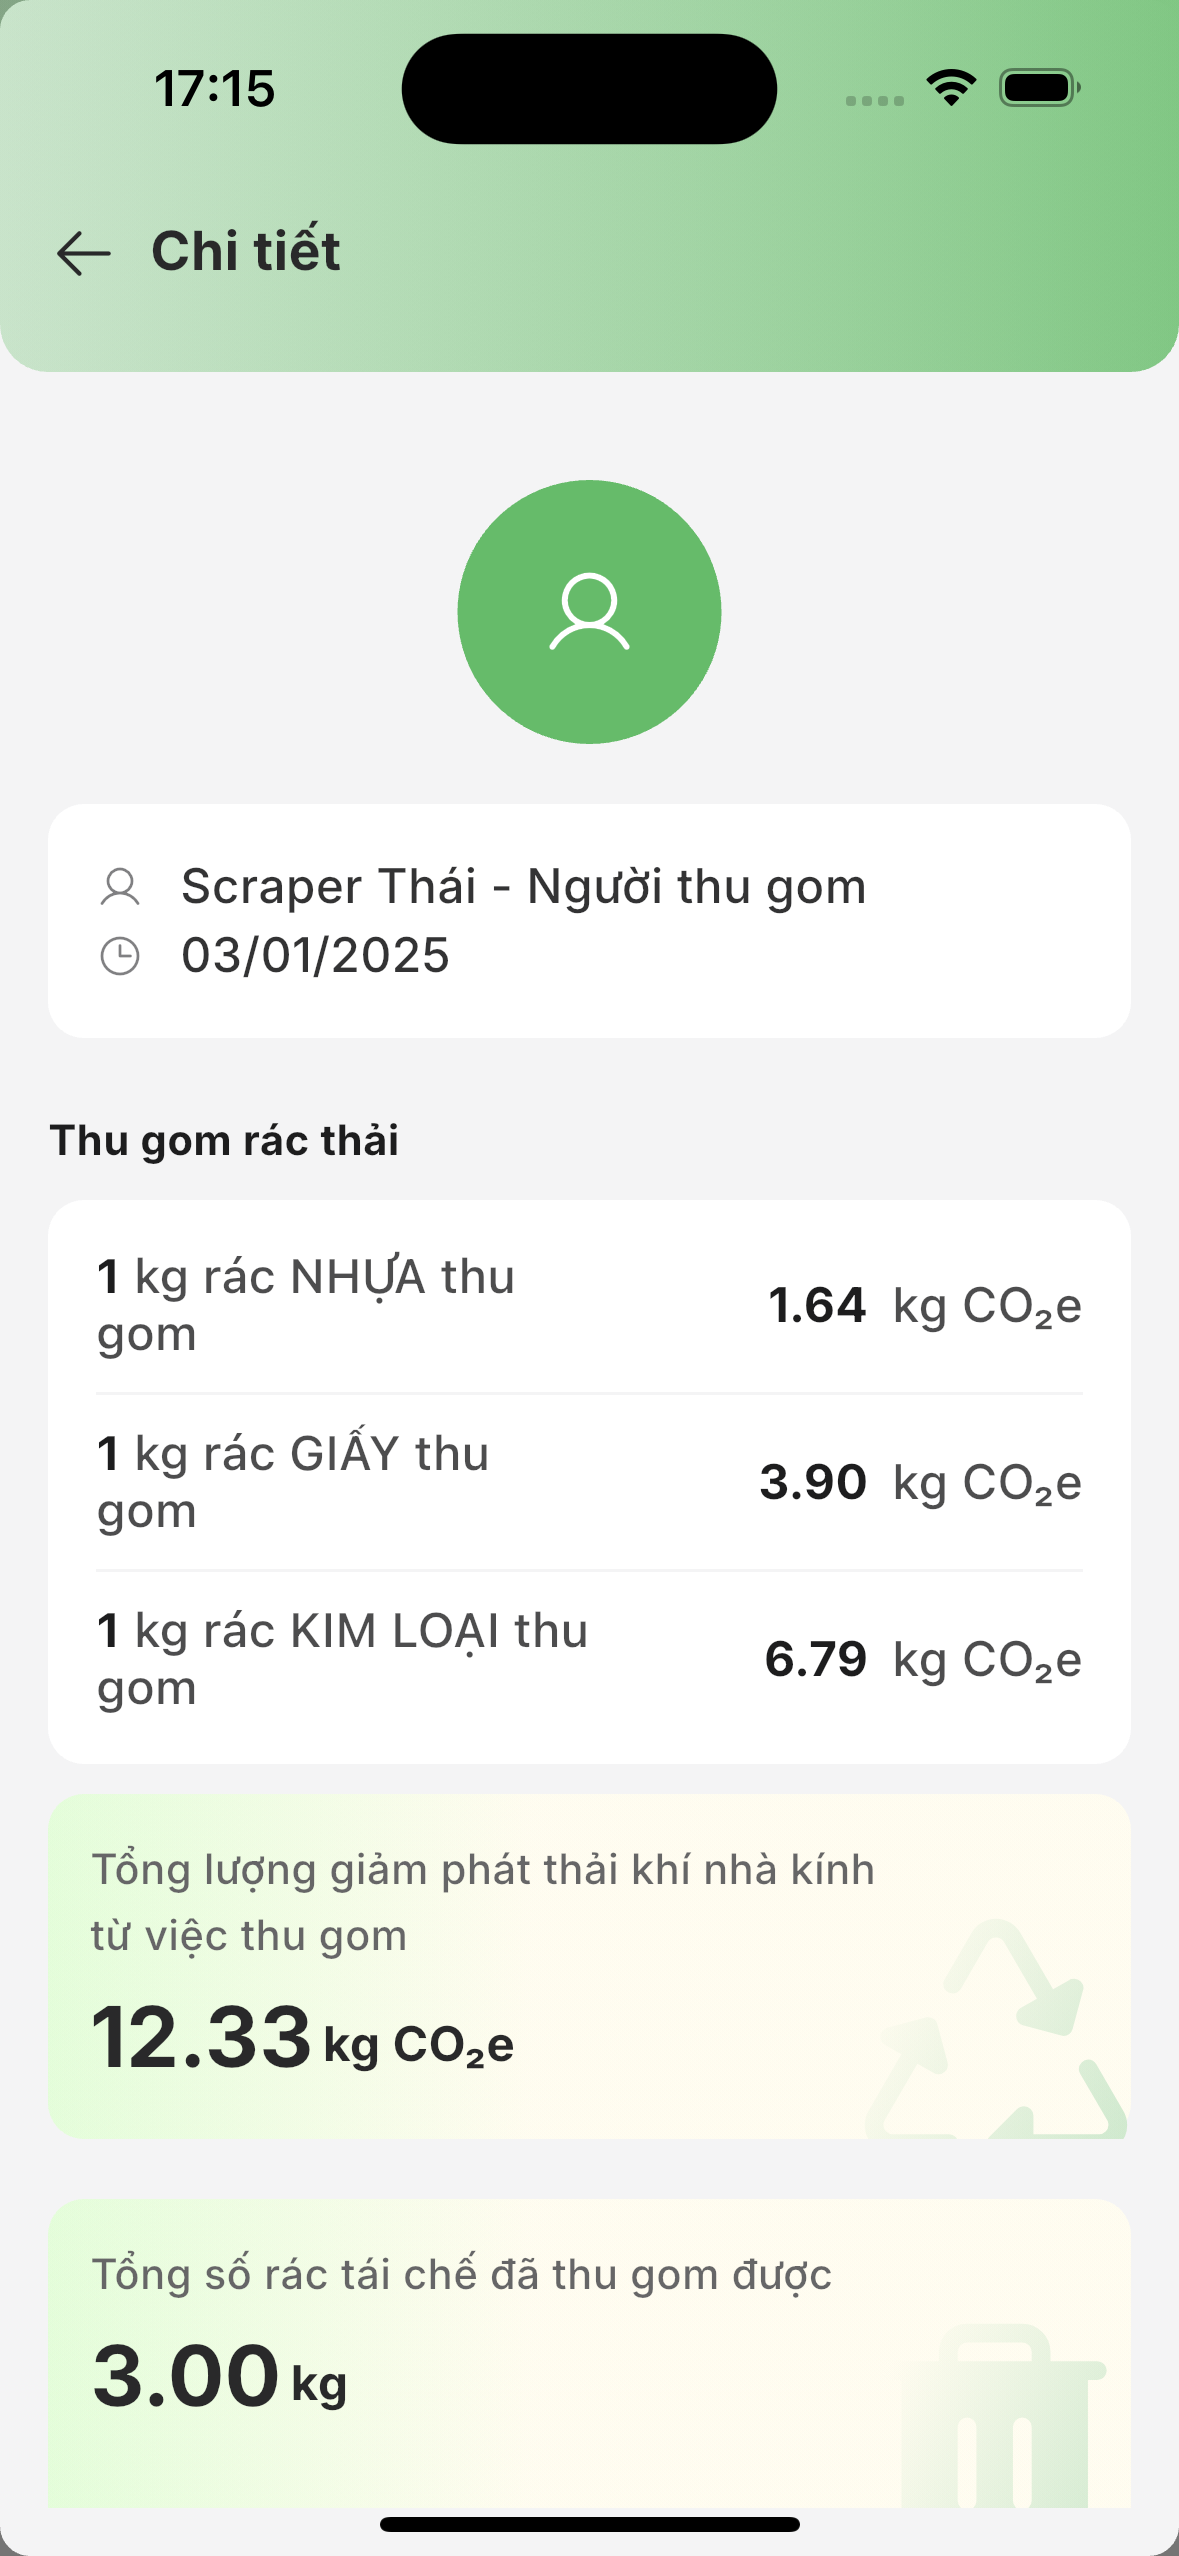
\includegraphics[width=0.45\textwidth]{Images/mobile/contribution_detail_screen.png}}%
  \caption[Hình ảnh màn thống kê/chi tiết đóng góp]{\bfseries \fontsize{12pt}{0pt}
  \selectfont Hình ảnh màn thống kê/chi tiết đóng góp}
  \label{contribution_detail_waznet}
\end{figure}

\subsubsection{Chức năng lọc số liệu đã nhập theo khoảng thời gian}
Đối với Hộ gia đình, nhấn vào tab \textbf{Số liệu}, bên cạnh dòng \textbf{Thống kê số liệu đóng góp}, nhấn vào button màu xám, bộ lọc sẽ hiện lên

Đối với Hộ gia đình, ở trang chủ, kéo xuống hoặc nhấn vào tab \textbf{Số liệu}, bên cạnh dòng \textbf{Thống kê số liệu đóng góp}, sau đó nhấn vào button màu xám, bộ lọc sẽ hiện lên.

\begin{figure}[H]
  \centering
  \subcaptionbox{Màn danh sách đóng góp}{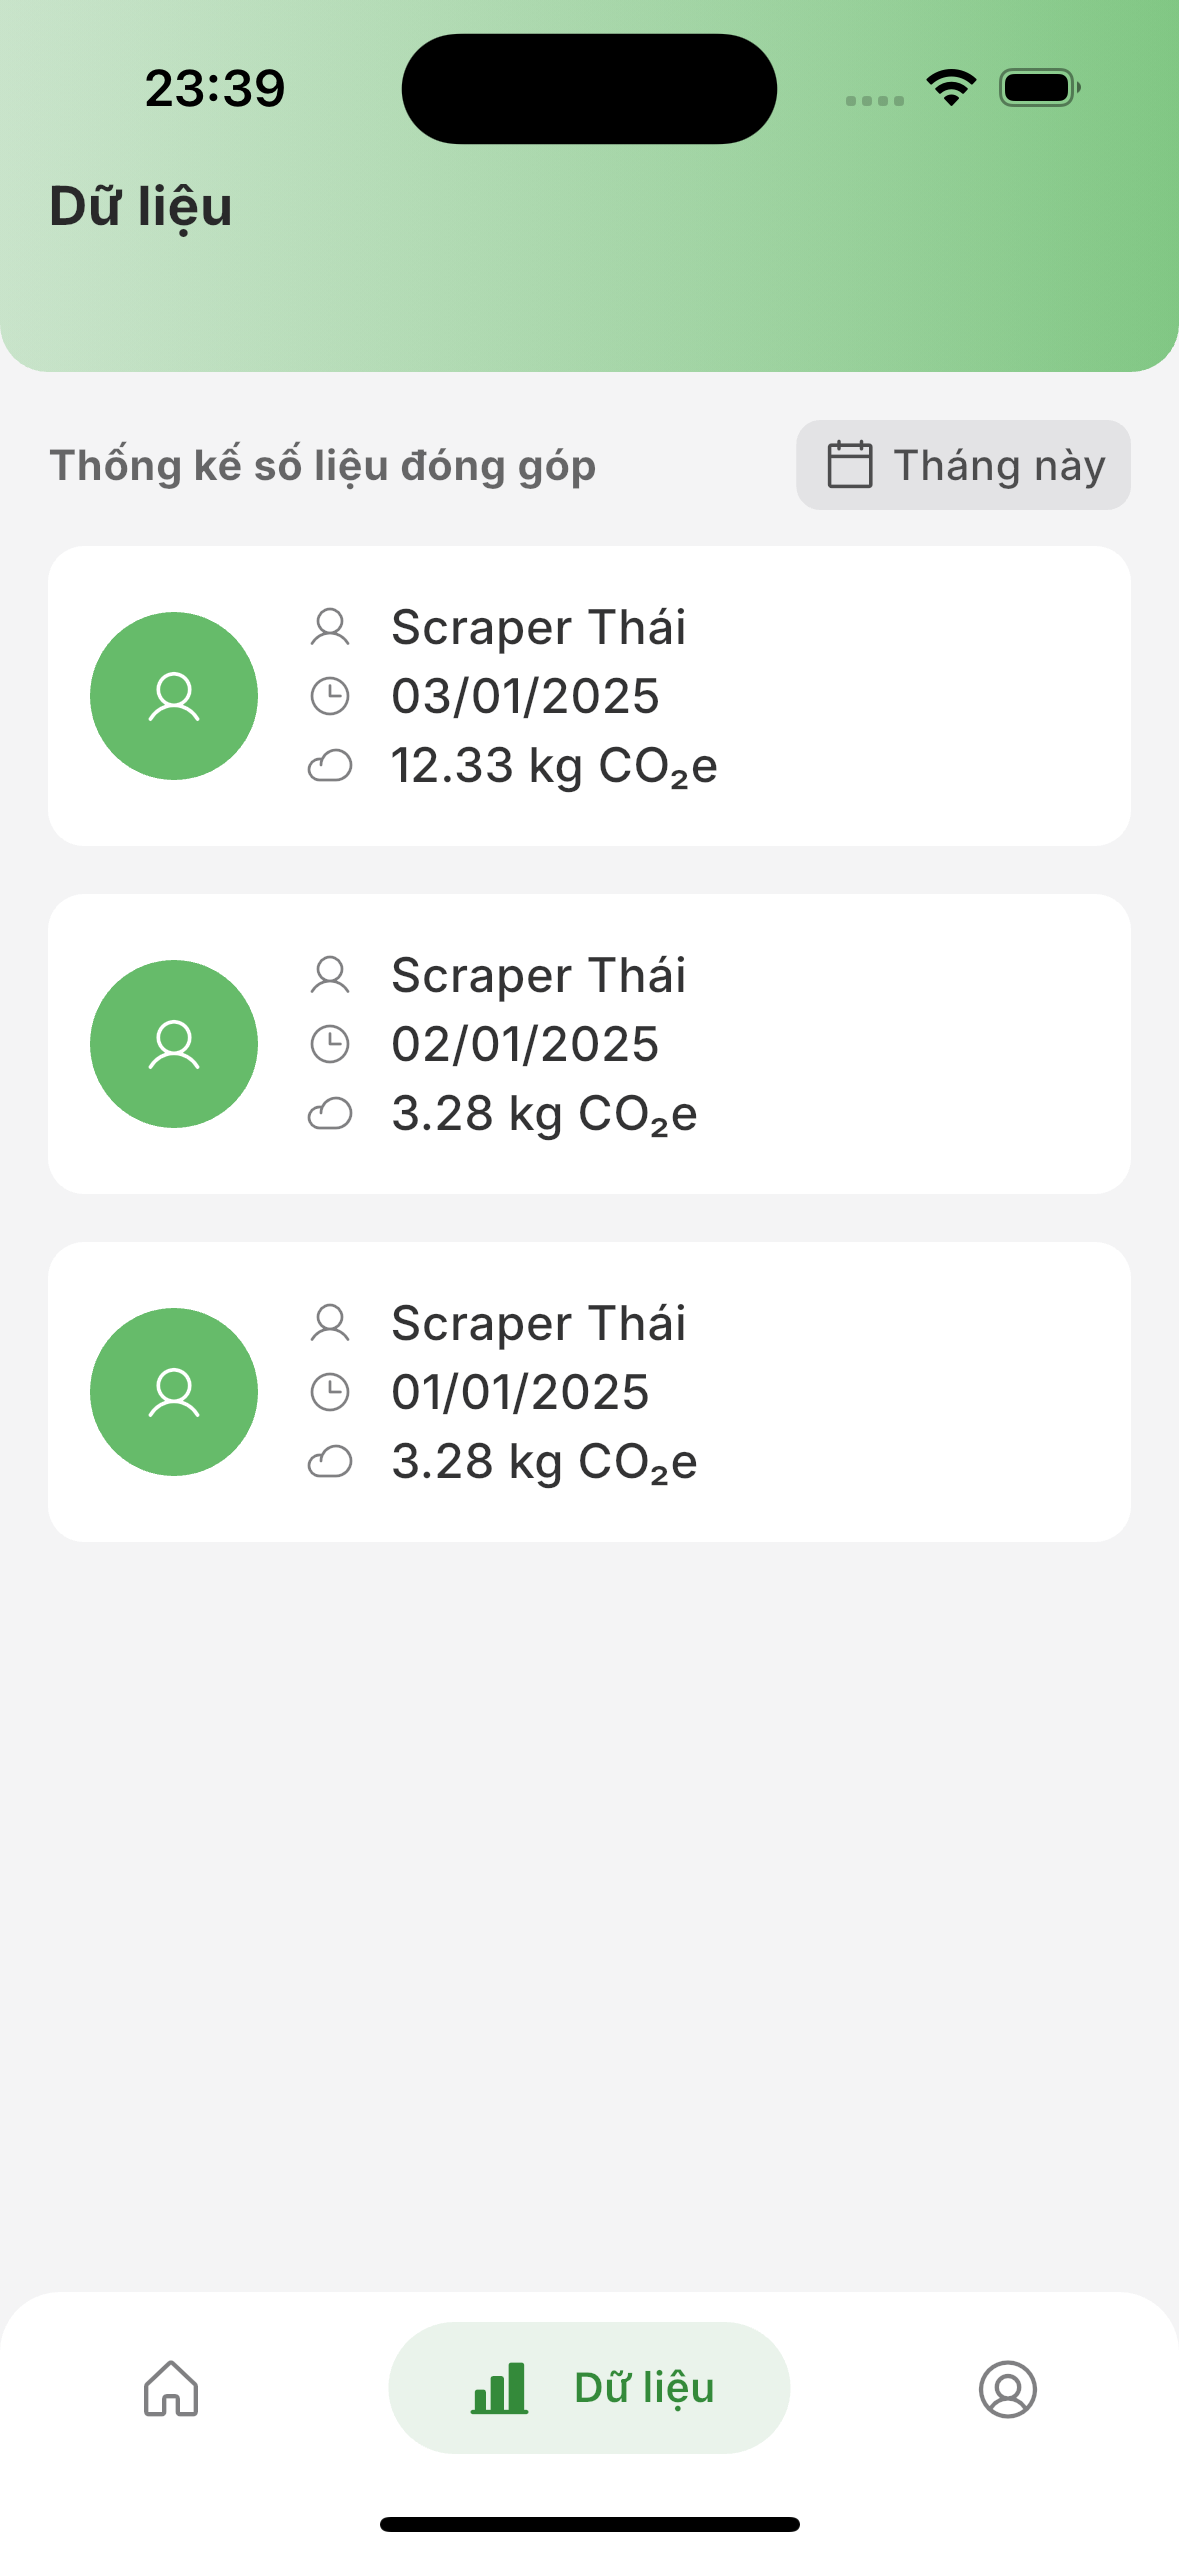
\includegraphics[width=0.32\textwidth]{Images/mobile/contributions_screen.png}}%
  \hfill
  \subcaptionbox{Các option chọn thời gian}{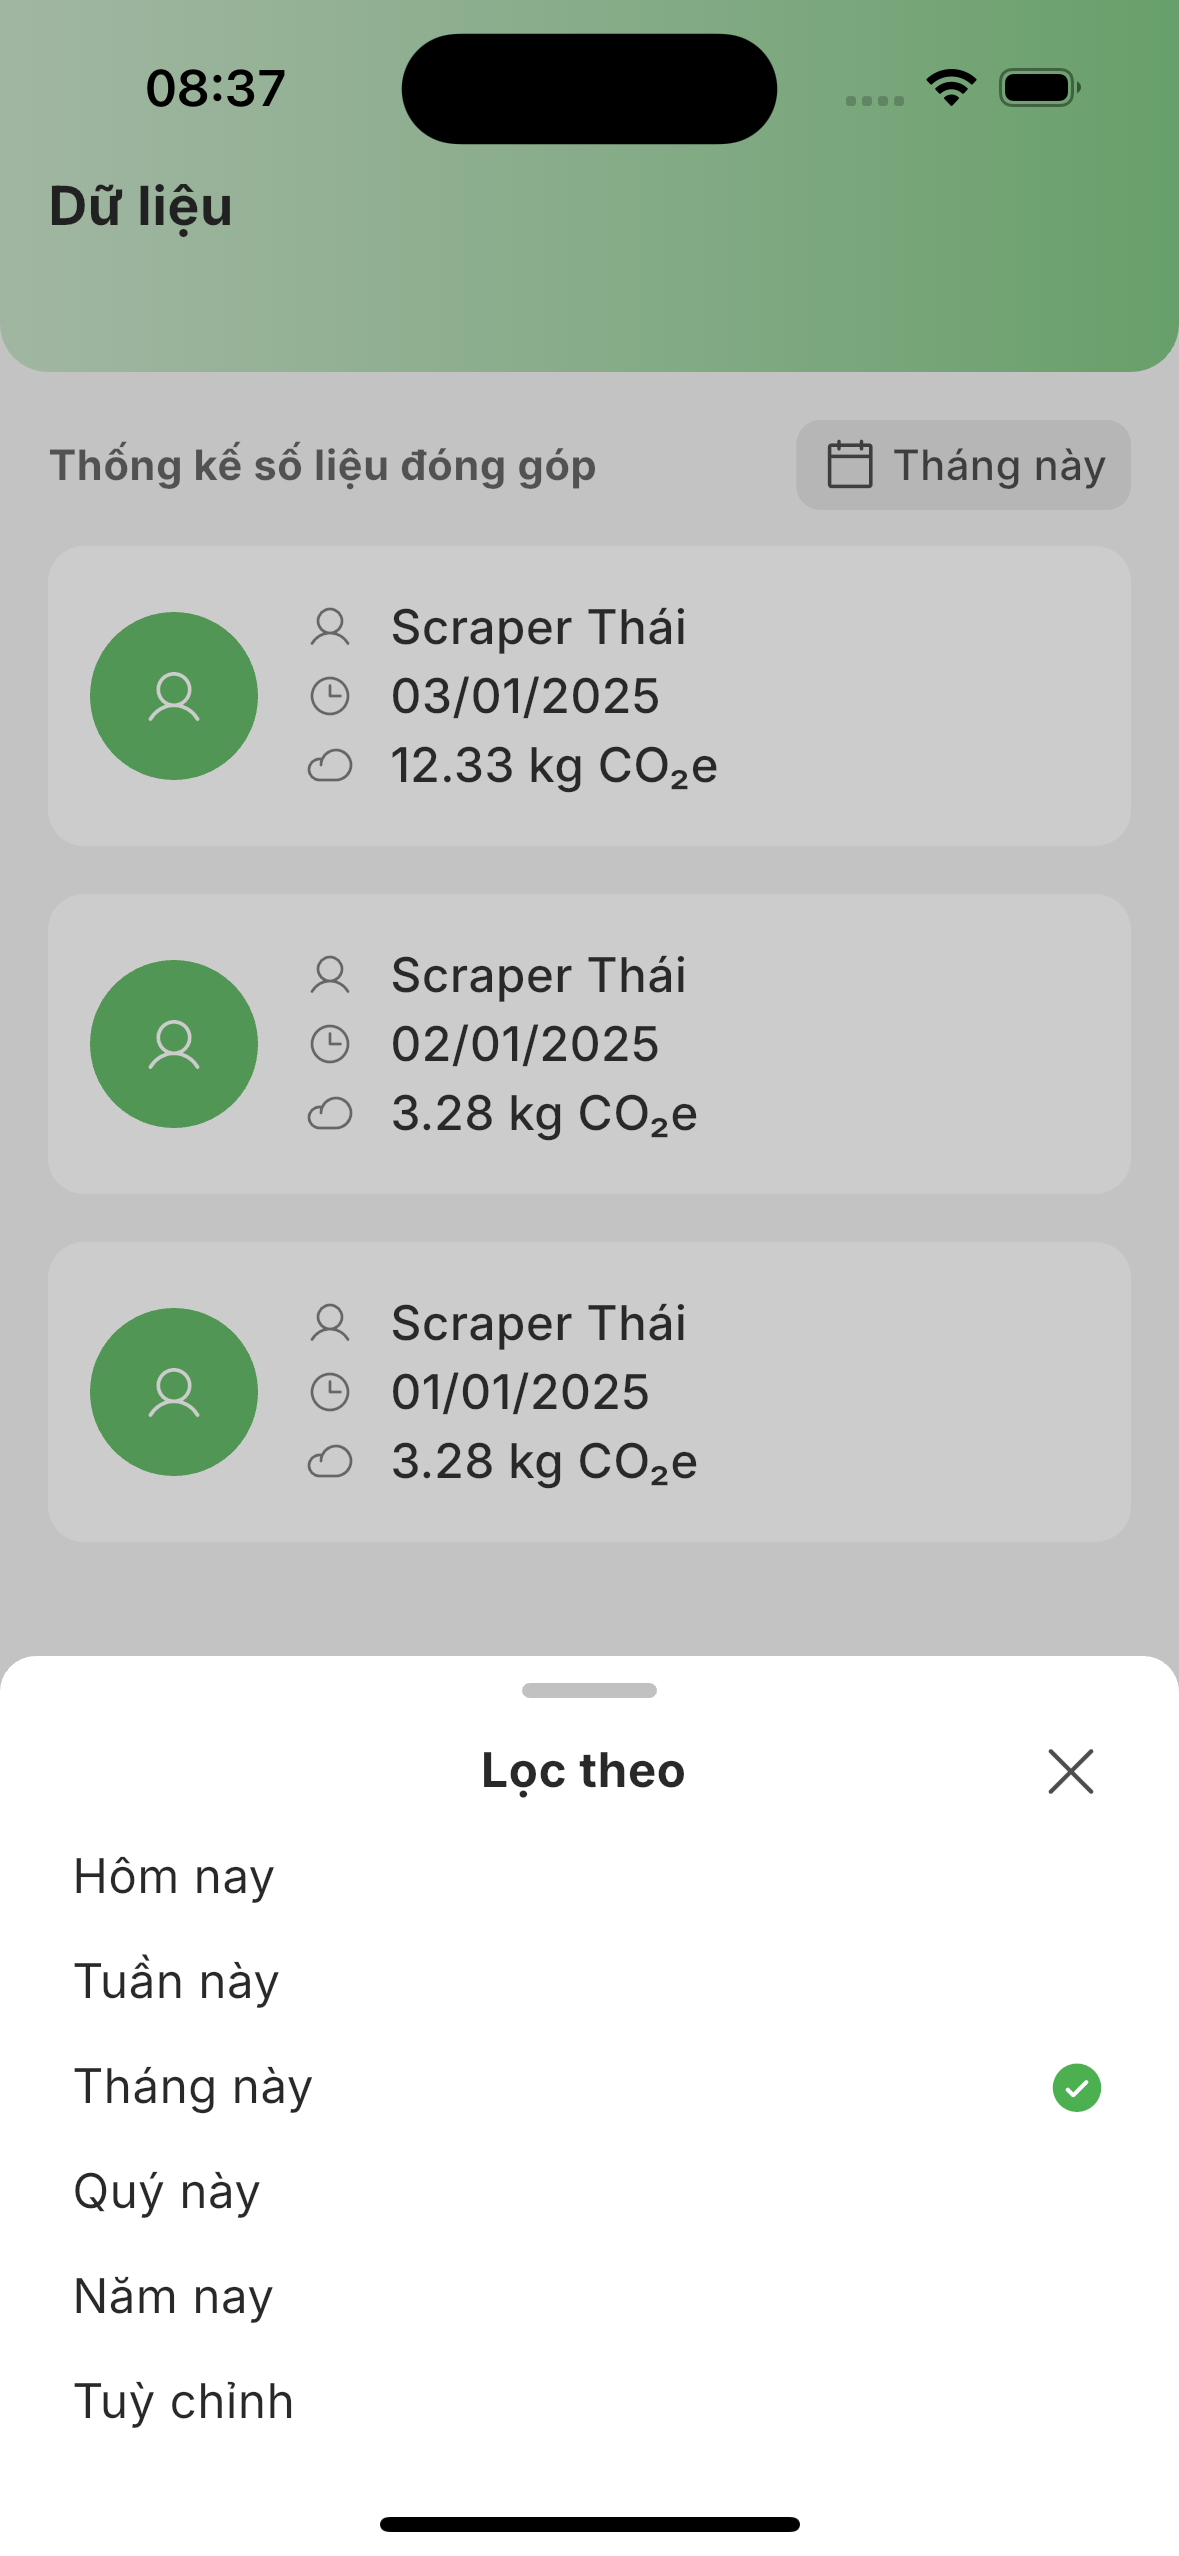
\includegraphics[width=0.32\textwidth]{Images/mobile/filter_date_0.png}}%
  \hfill
  \subcaptionbox{Chọn theo khoảng thời gian custom}{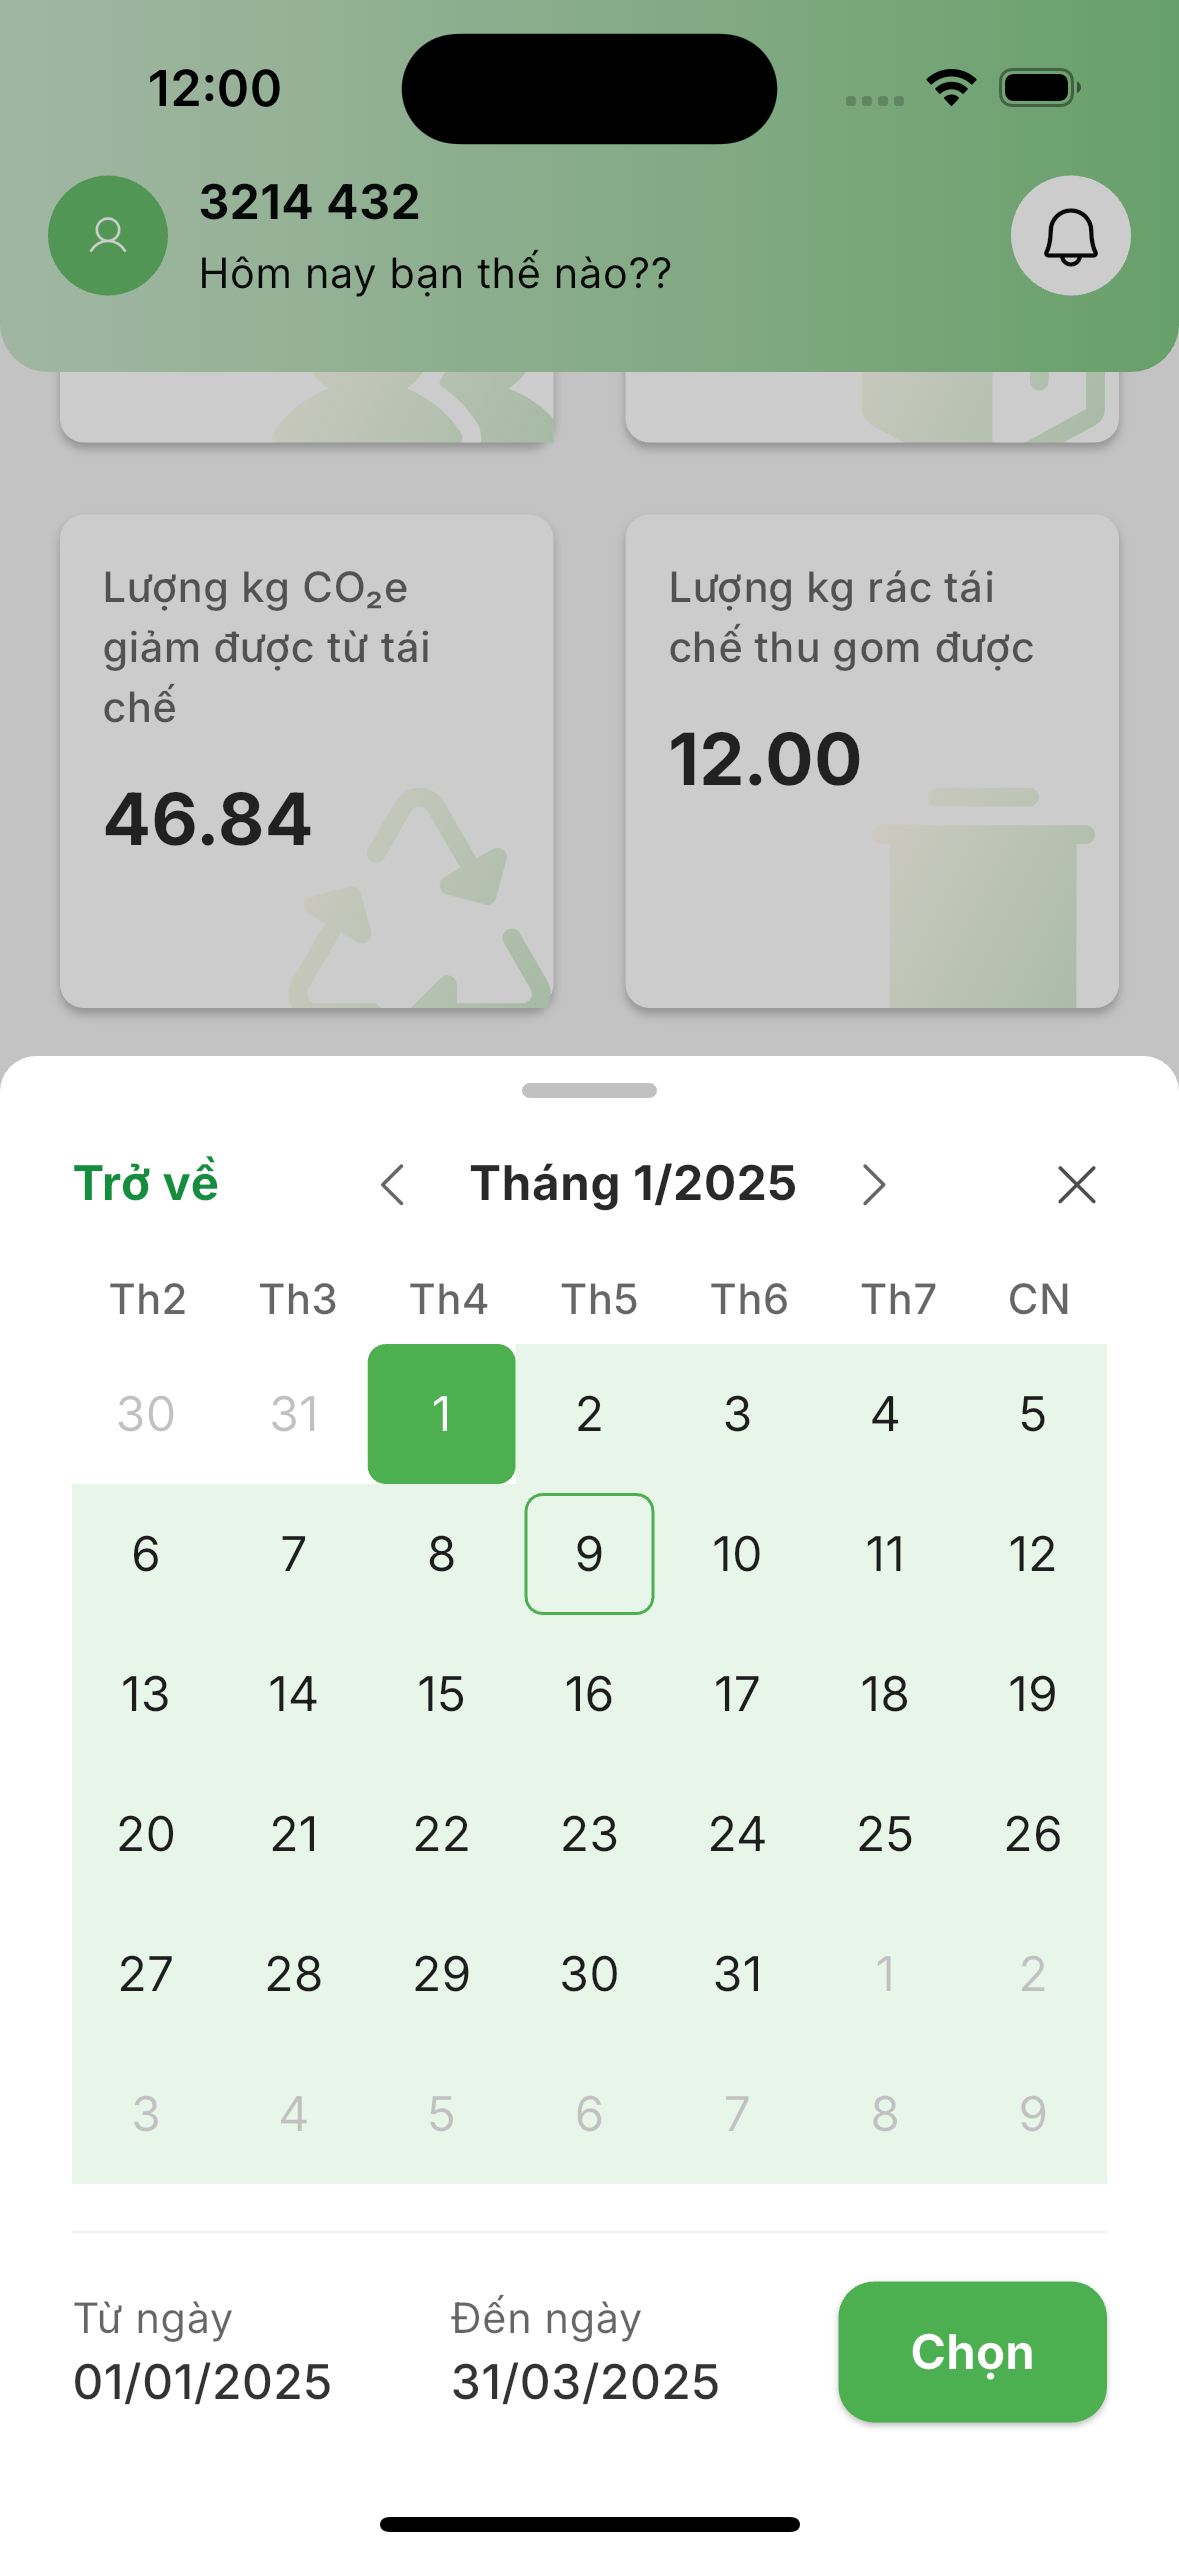
\includegraphics[width=0.32\textwidth]{Images/mobile/filter_date.png}}%
  \caption[Hình ảnh màn chức năng lọc số liệu]{\bfseries \fontsize{12pt}{0pt}
  \selectfont Hình ảnh màn chức năng lọc số liệu}
  \label{contribution_filter_waznet}
\end{figure}

\subsubsection{Chức năng sửa thông tin người dùng}
Nhấn vào tab \textbf{Tài khoản}, chọn sửa thông tin, ứng dụng sẽ đưa người dùng sang trang sửa thông tin, người dùng sửa và nhấn nút lưu.
\begin{figure}[H]
  \centering
  \subcaptionbox{Màn danh sách đóng góp}{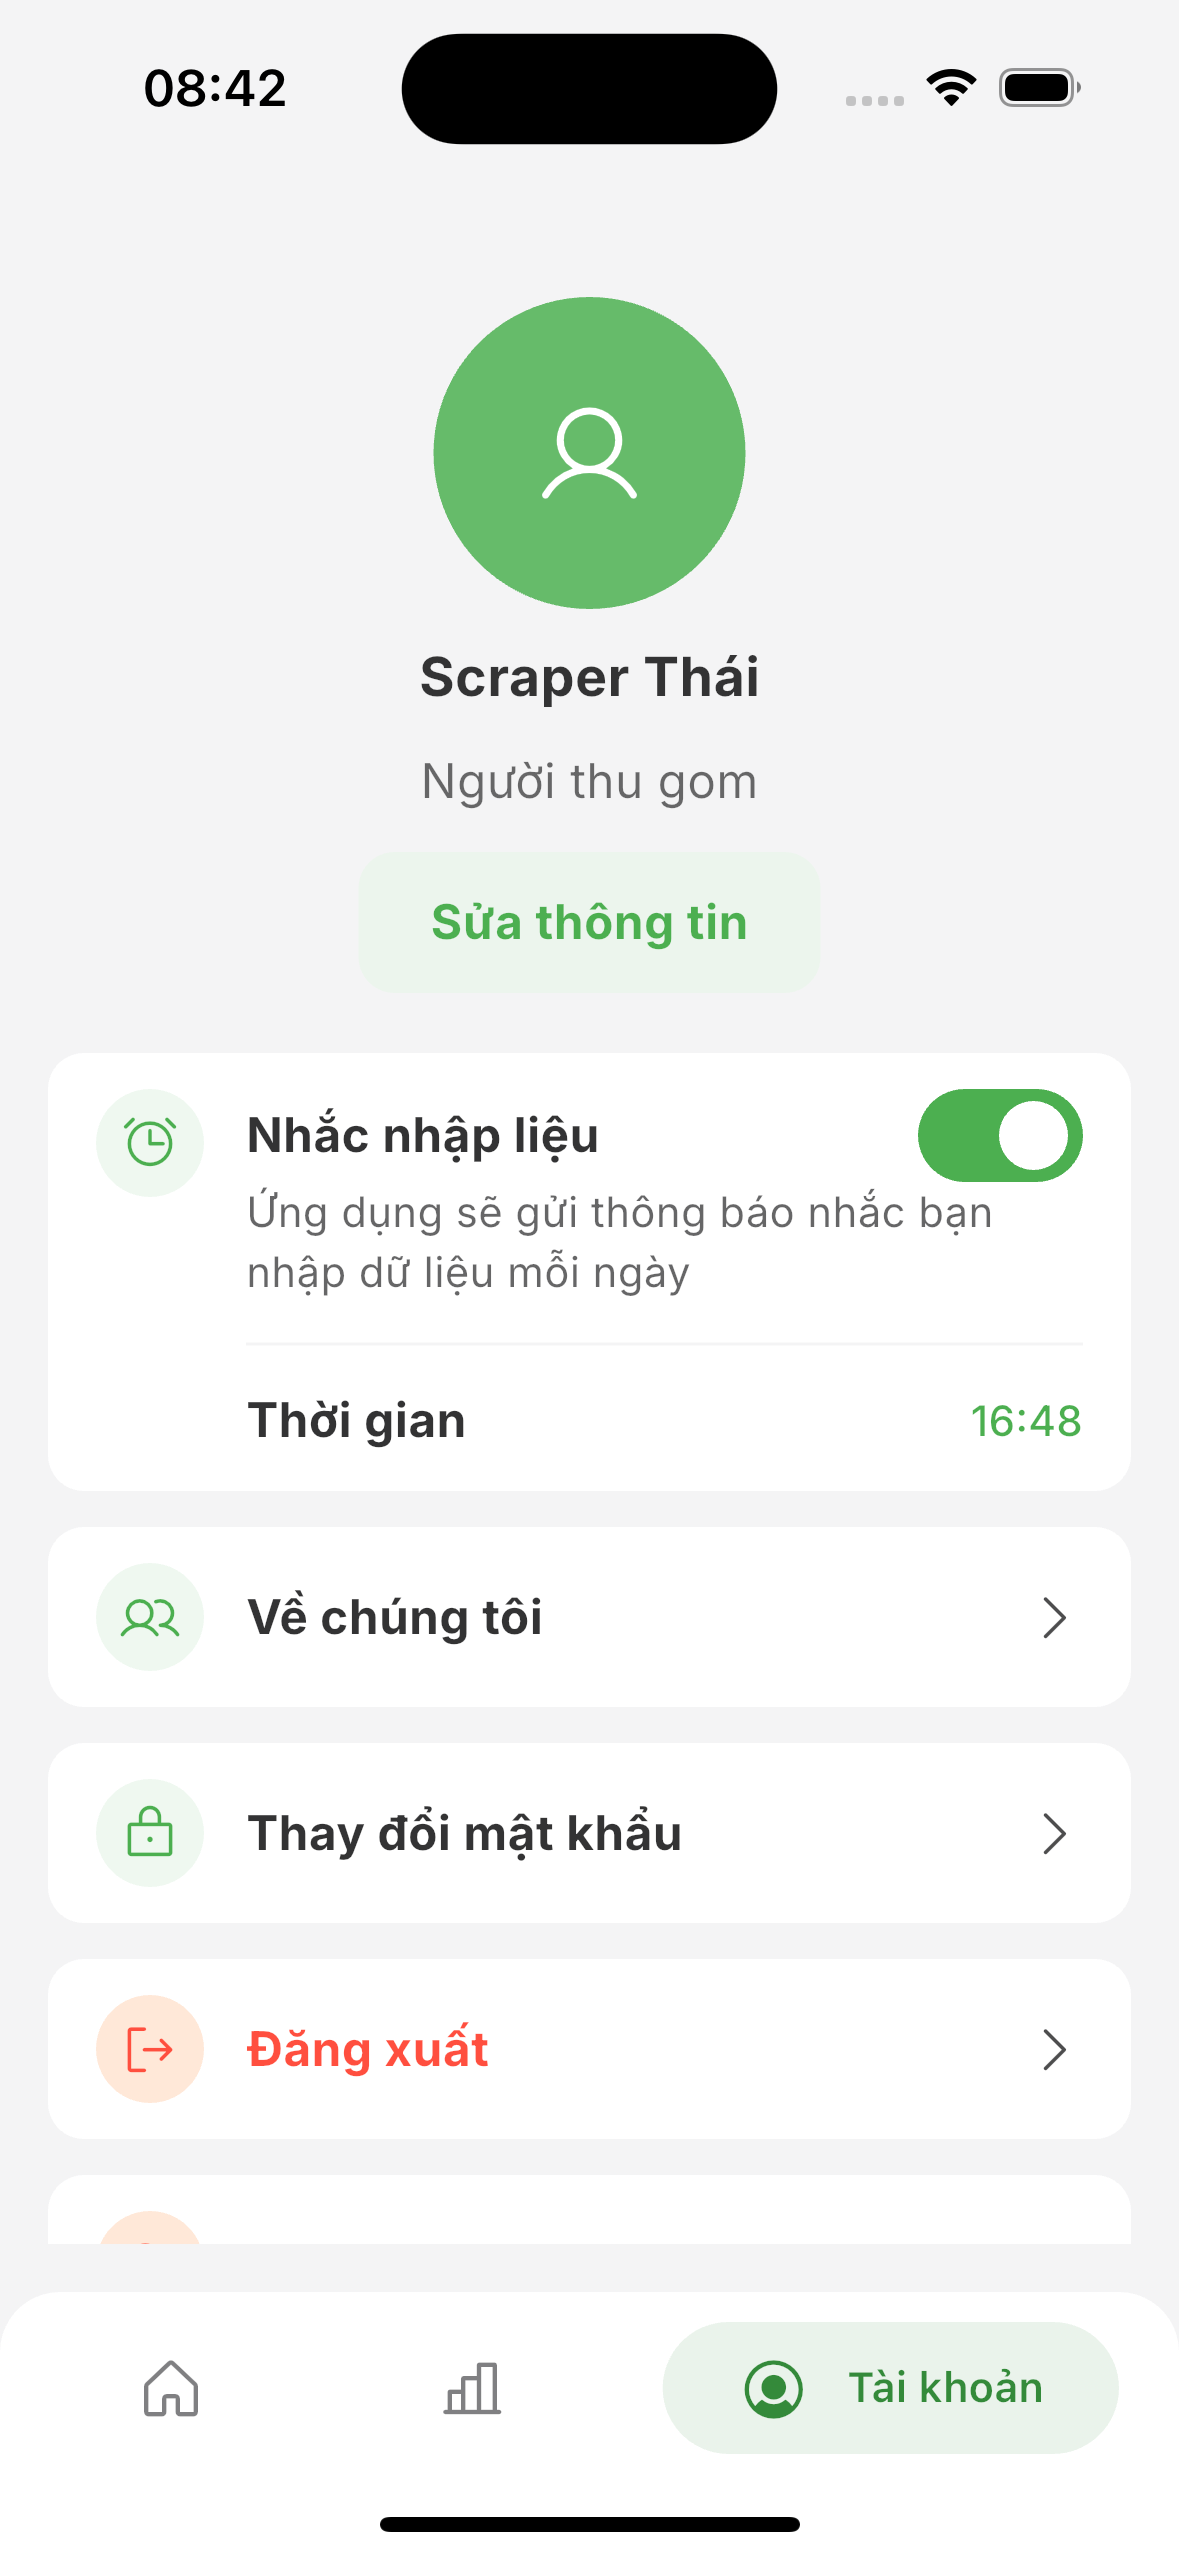
\includegraphics[width=0.45\textwidth]{Images/mobile/account_screen.png}}%
  \hfill
  \subcaptionbox{Màn chi tiết đóng góp trong một ngày}{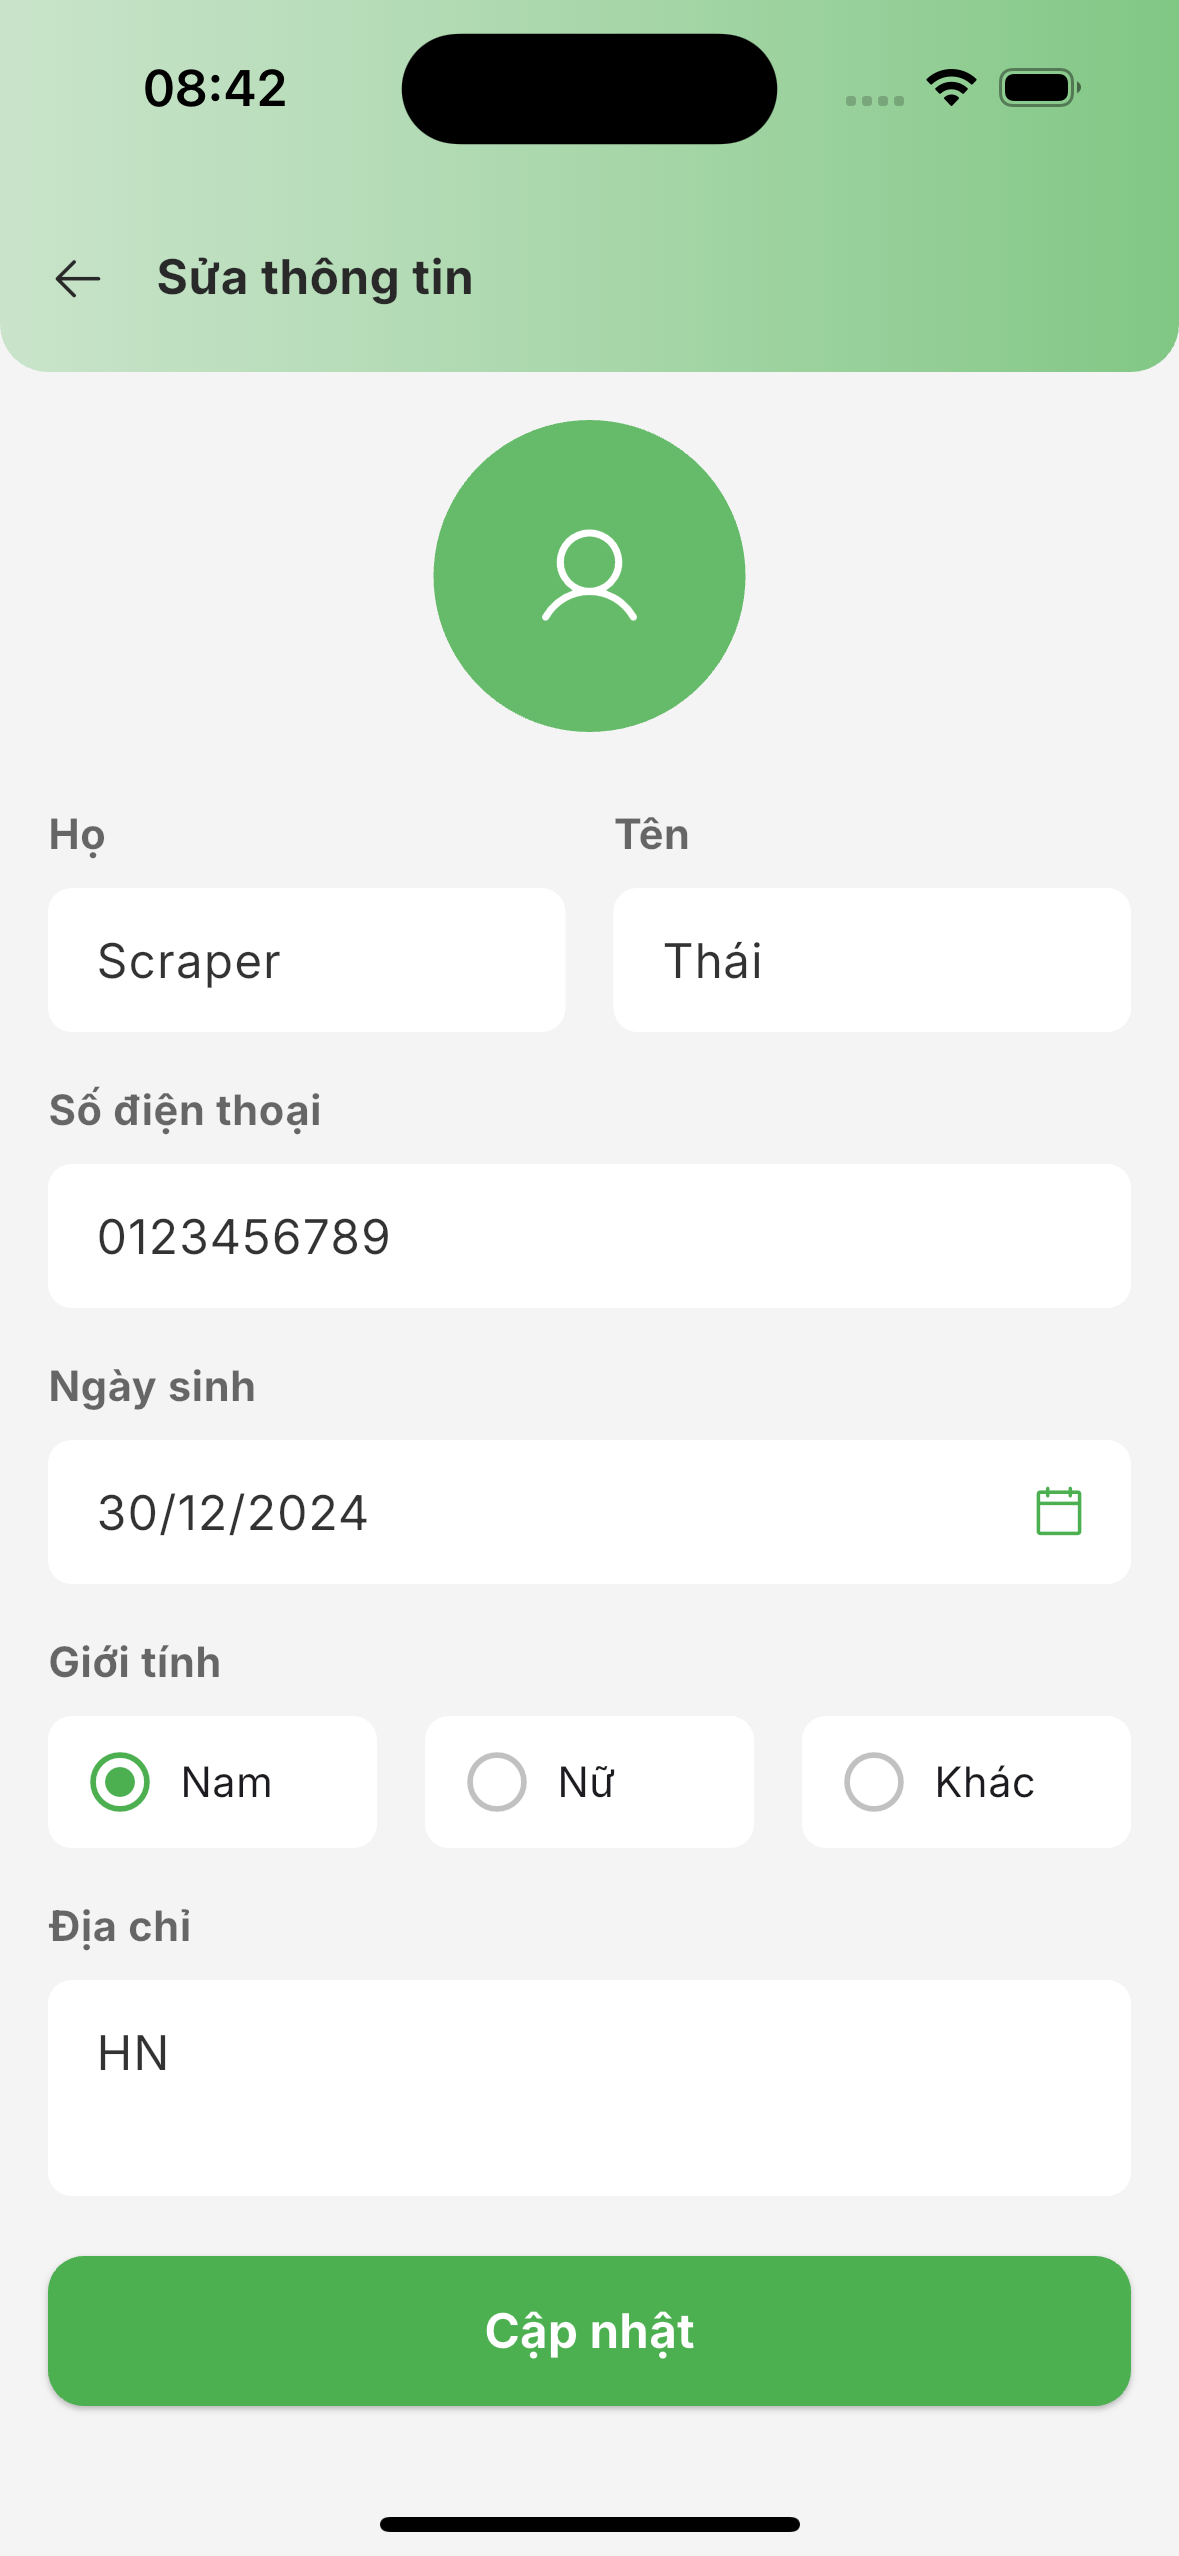
\includegraphics[width=0.45\textwidth]{Images/mobile/edit_info_screen.png}}%
  \caption[Hình ảnh màn sửa thông tin người dùng]{\bfseries \fontsize{12pt}{0pt}
  \selectfont Hình ảnh màn sửa thông tin người dùng}
  \label{user_info_edit_waznet}
\end{figure}
\subsubsection{Chức năng đổi ảnh đại diện}
Chức năng đang được bổ sung.
\subsubsection{Chức năng đổi mật khẩu}
Người dùng nhấn vào tab \textbf{Tài khoản}, chọn thay đổi mật khẩu, ứng dụng sẽ đưa người dùng sang trang đổi mật khẩu, người dùng cần nhập mật khẩu chính xác mật khẩu hiện tại, sau đó mới có thể đổi mật khẩu.
\begin{figure}[H]
  \centering
  \subcaptionbox{Màn danh sách đóng góp}{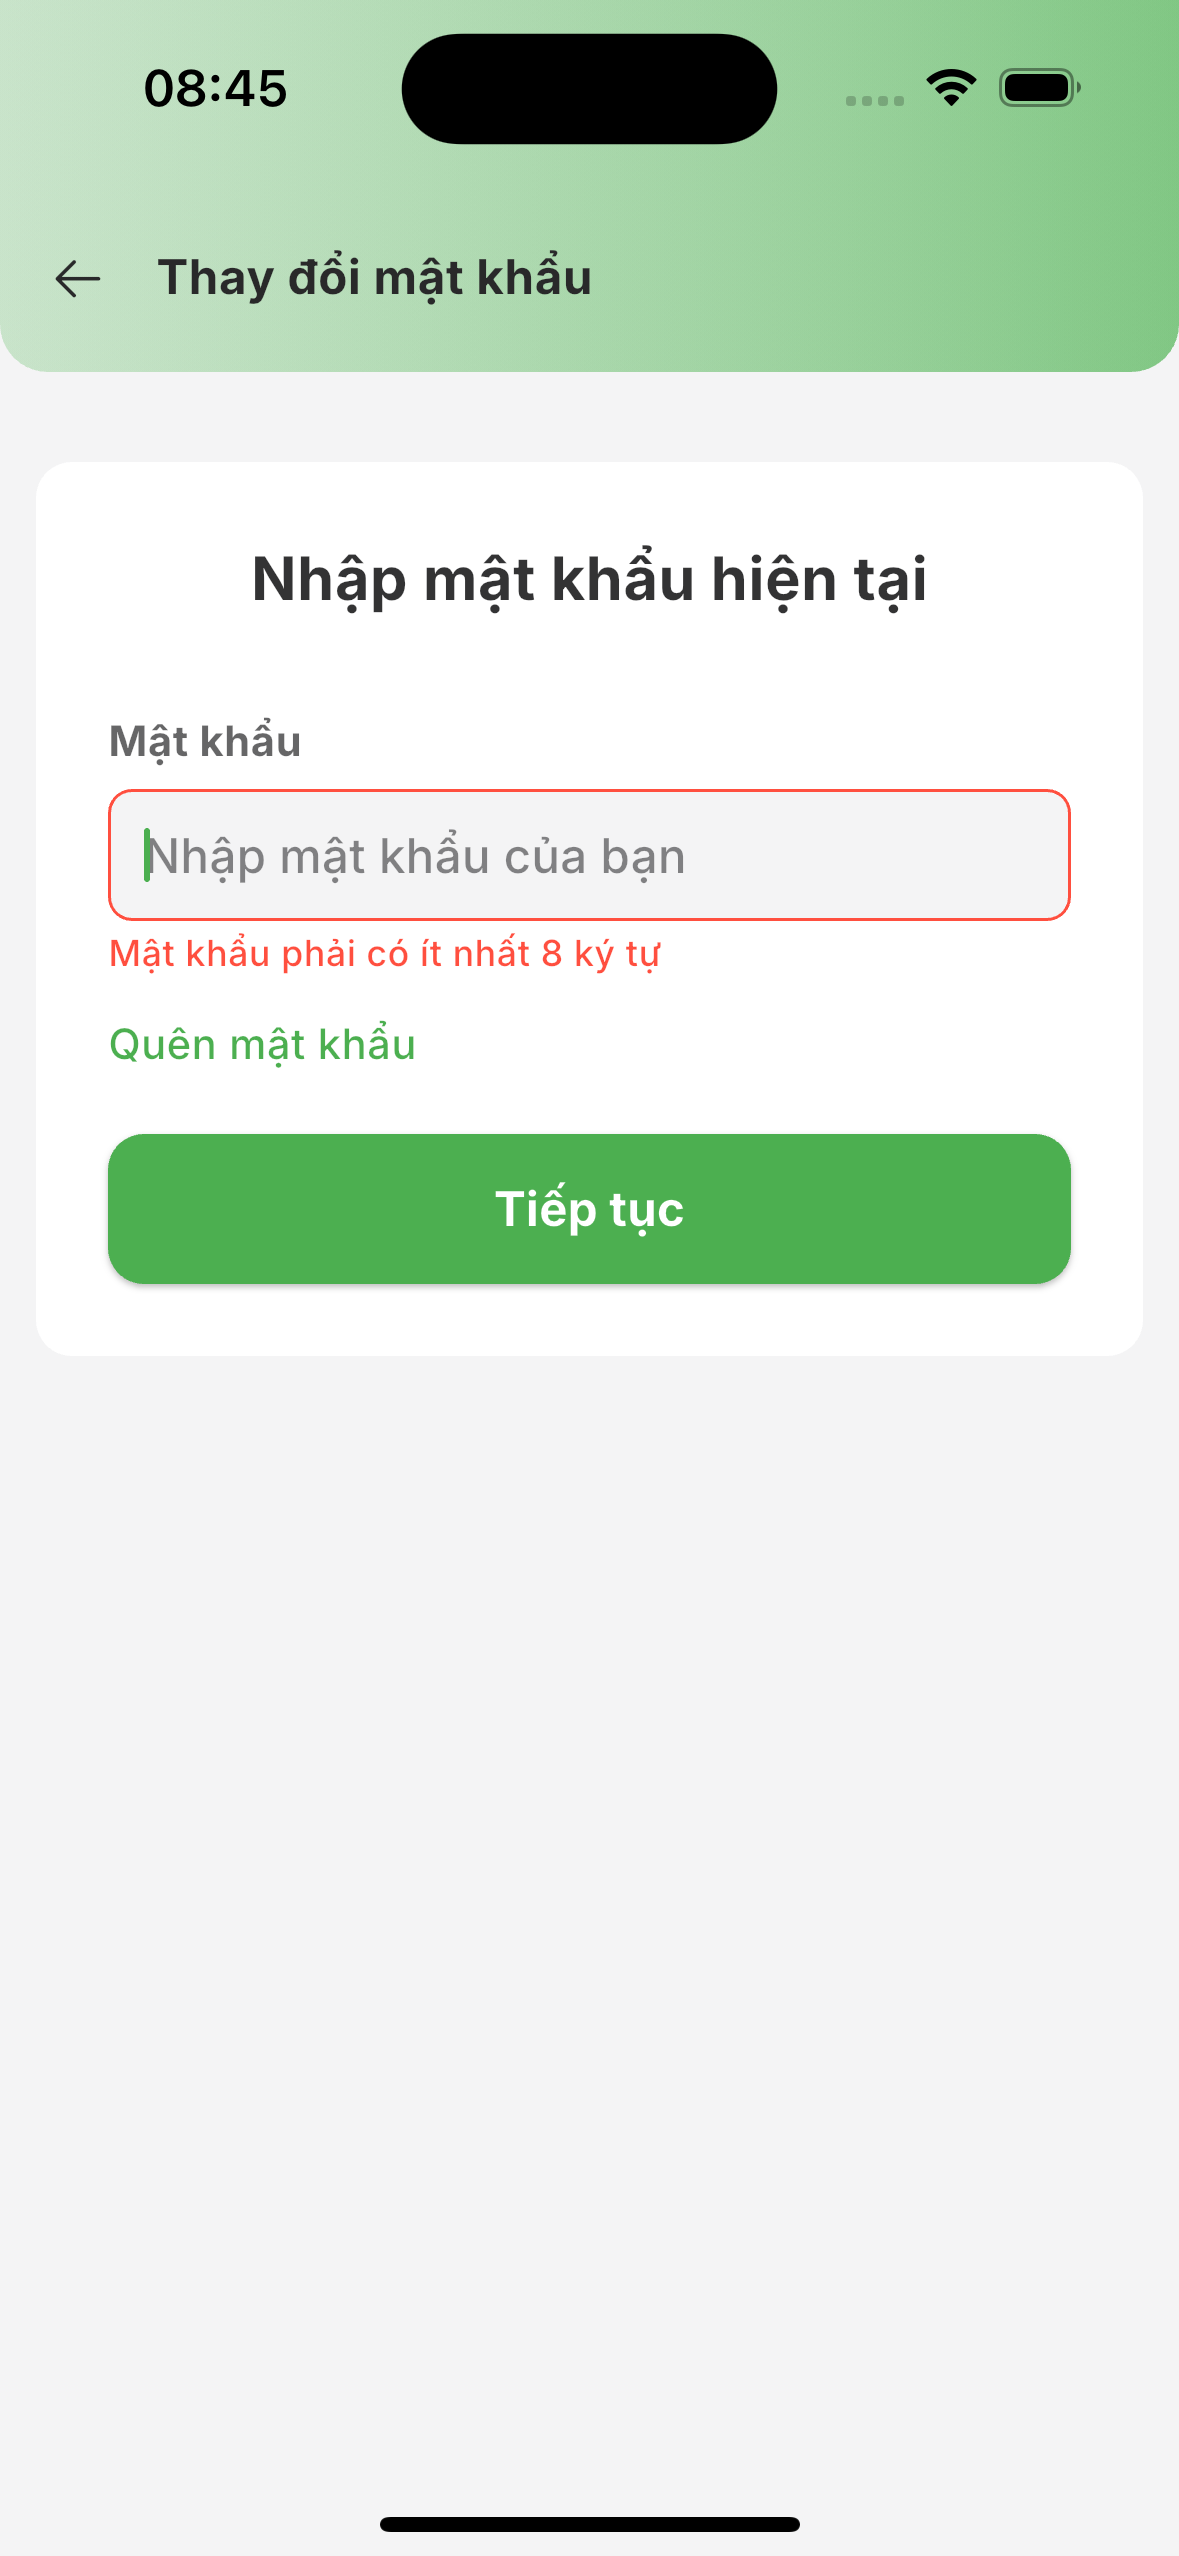
\includegraphics[width=0.45\textwidth]{Images/mobile/change_password_screen.png}}%
  \hfill
  \subcaptionbox{Màn chi tiết đóng góp trong một ngày}{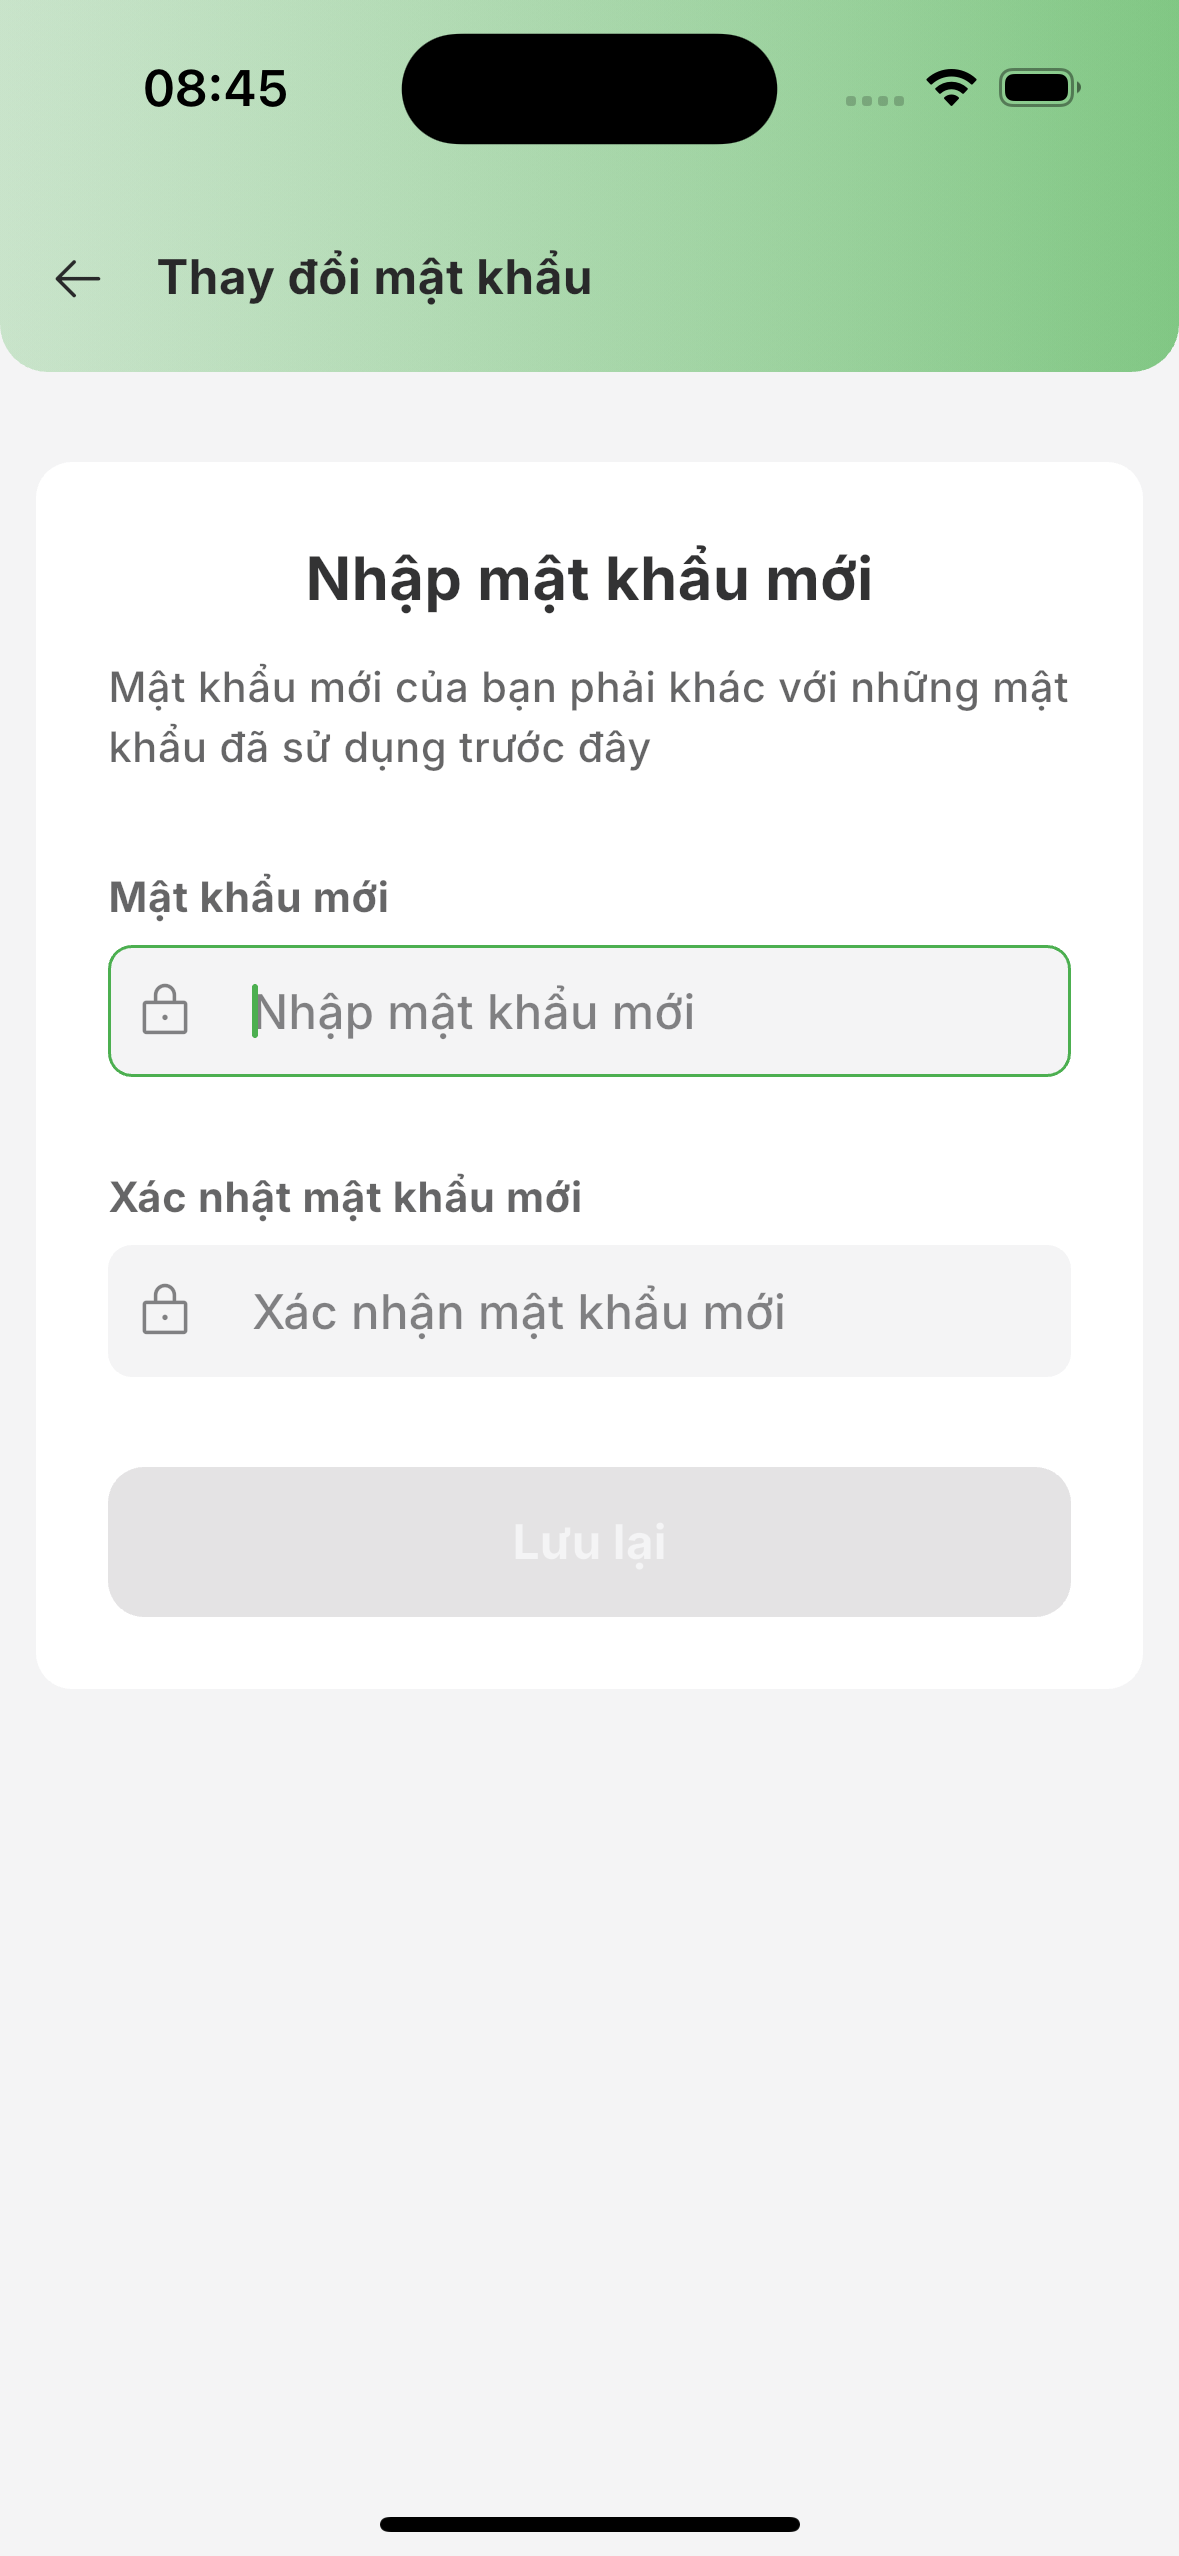
\includegraphics[width=0.45\textwidth]{Images/mobile/change_password_screen_2.png}}%
  \caption[Hình ảnh màn chức năng đổi mật khẩu]{\bfseries \fontsize{12pt}{0pt}
  \selectfont Hình ảnh màn chức năng đổi mật khẩu}
  \label{change_password_waznet}
\end{figure}
\subsubsection{Chức năng đăng xuất}
Người dùng nhấn vào tab \textbf{Tài khoản}, chọn đăng xuất, ứng dụng sẽ đưa ra cảnh báo, người dùng nhấn \textbf{Xác nhận} để thực hiện đăng xuất khỏi tài khoản. Sau khi đăng xuất, người dùng sẽ được đưa về màn đăng nhập.
\begin{figure}[H]
  \centering
  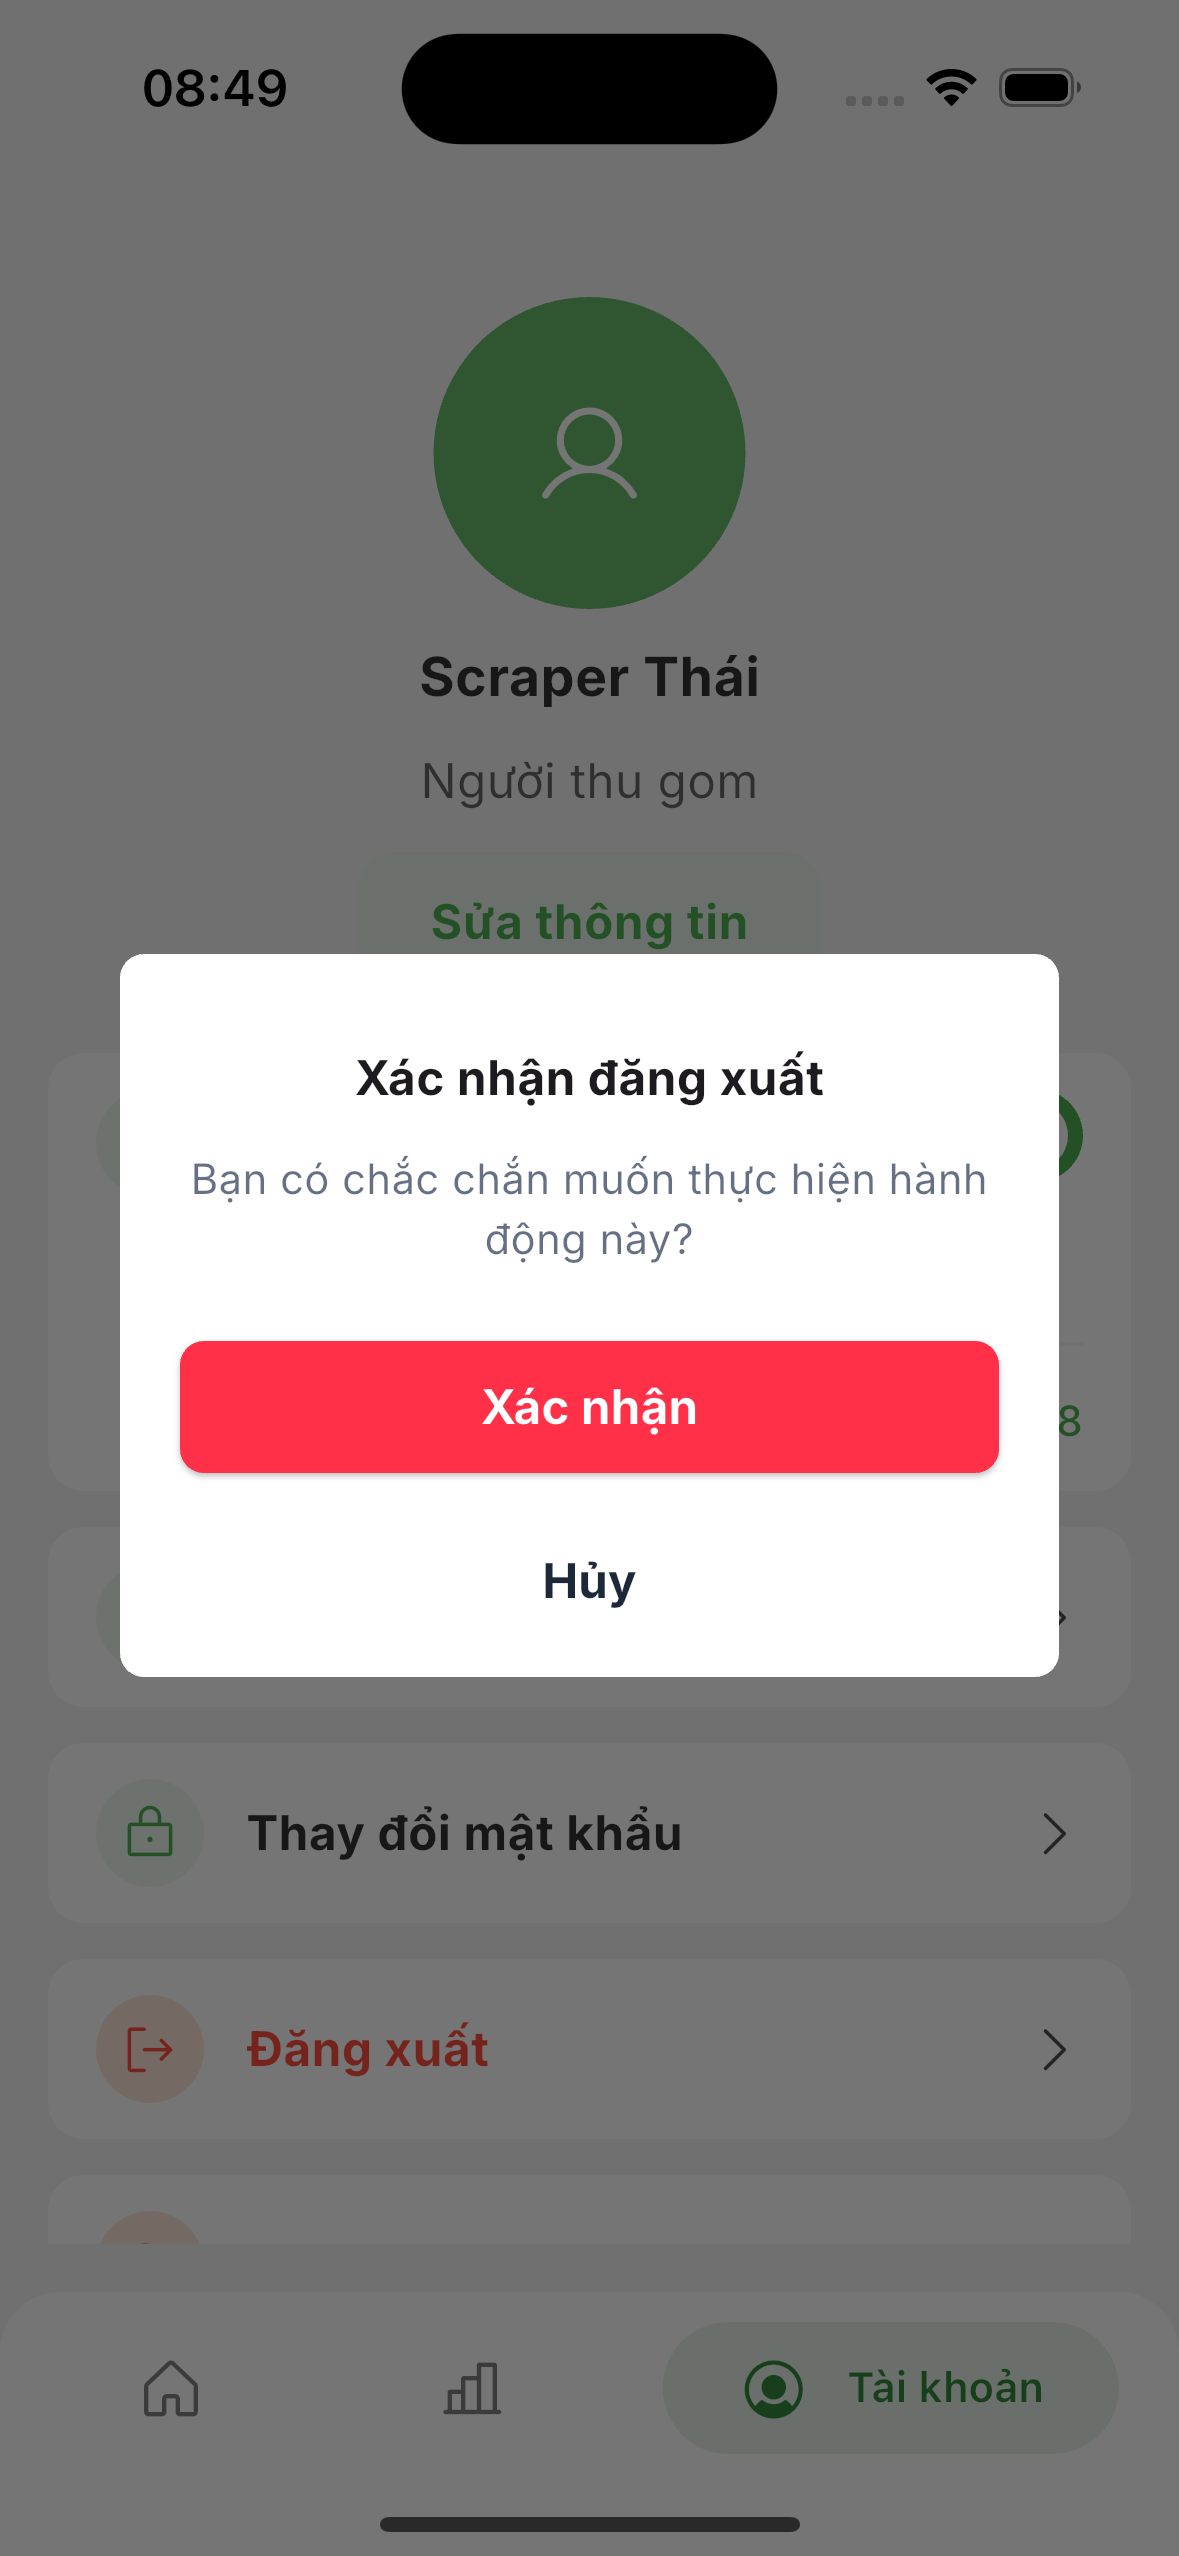
\includegraphics[width=0.45\textwidth]{Images/mobile/logout_dialog.png}
  \caption[Hình ảnh thông báo xác nhận đăng xuất]{\bfseries \fontsize{12pt}{0pt}
  \selectfont Hình ảnh thông báo xác nhận đăng xuất}
  \label{logout_dialog} %đặt tên cho ảnh
\end{figure}
\subsubsection{Chức năng xoá tài khoản}
Người dùng nhấn vào tab \textbf{Tài khoản}, chọn xoá tài khoản, ứng dụng sẽ đưa ra cảnh báo, người dùng nhấn \textbf{Xác nhận} để thực hiện xoá tài khoản. \textbf{Người dùng lưu ý}, việc xoá tài khoản sẽ xoá tài khoản và vẫn giữ lại dữ liệu đóng góp, người dùng sẽ không thể đăng ký lại tài khoản với số điện thoại đã xoá.
\begin{figure}[H]
  \centering
  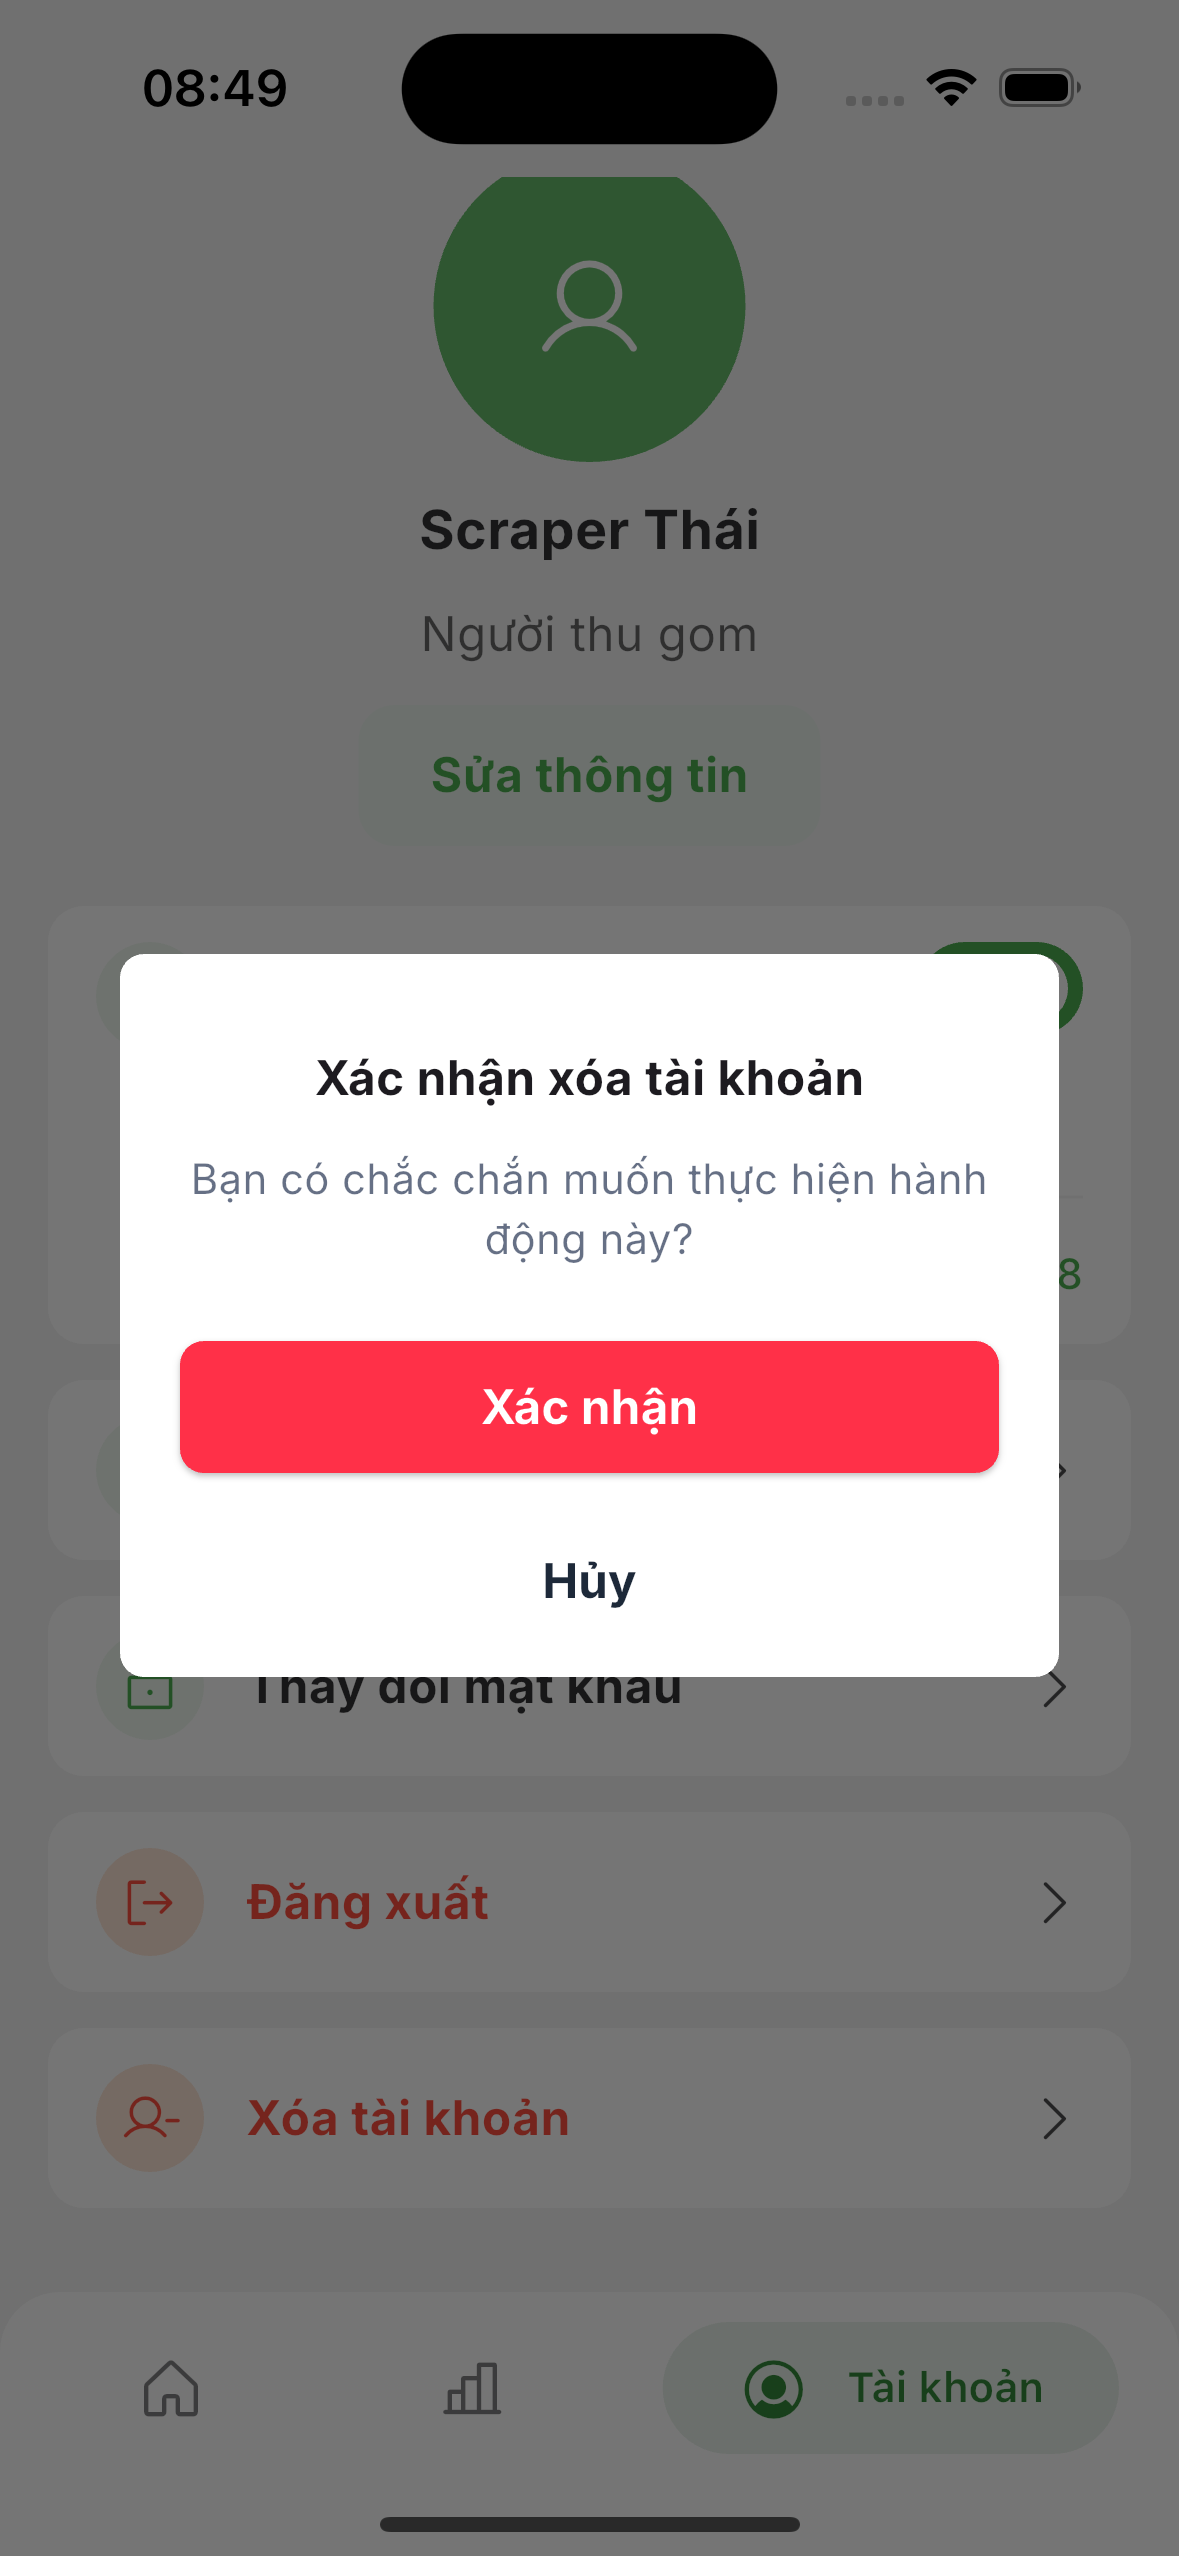
\includegraphics[width=0.45\textwidth]{Images/mobile/delete_account_dialog.png}
  \caption[Hình ảnh thông báo xác nhận xoá tài khoản]{\bfseries \fontsize{12pt}{0pt}
  \selectfont Hình ảnh thông báo xác nhận xoá tài khoản}
  \label{delete_account_dialog} %đặt tên cho ảnh
\end{figure}
\subsection{Các chức năng riêng cho Hộ gia đình/Người thu gom}
\subsubsection{Chức năng nhập số liệu}
Người dùng nhấn vào tab \textbf{Trang chủ}, ở dưới cùng bên phải sẽ có một button dấu + hình tròn, người dùng nhấn vào, ứng dụng sẽ đưa người dùng sang trang nhập số liệu, người dùng nhập số liệu, tuỳ vào việc đăng ký là hộ gia đình hay người thu gom, các câu hỏi để nhập số liệu sẽ khác nhau.

Trong khi nhập số liệu, hệ thống sẽ tính toán lượng giảm phát thải khí nhà kính ngay lập tức cho người dùng.
Người dùng nhấn nút lưu để gửi số liệu lên hệ thống, khi thành công sẽ đưa người dùng về lại trang chủ.

\begin{figure}[H]
  \centering
  \subcaptionbox{Màn trang chủ với dấu +}{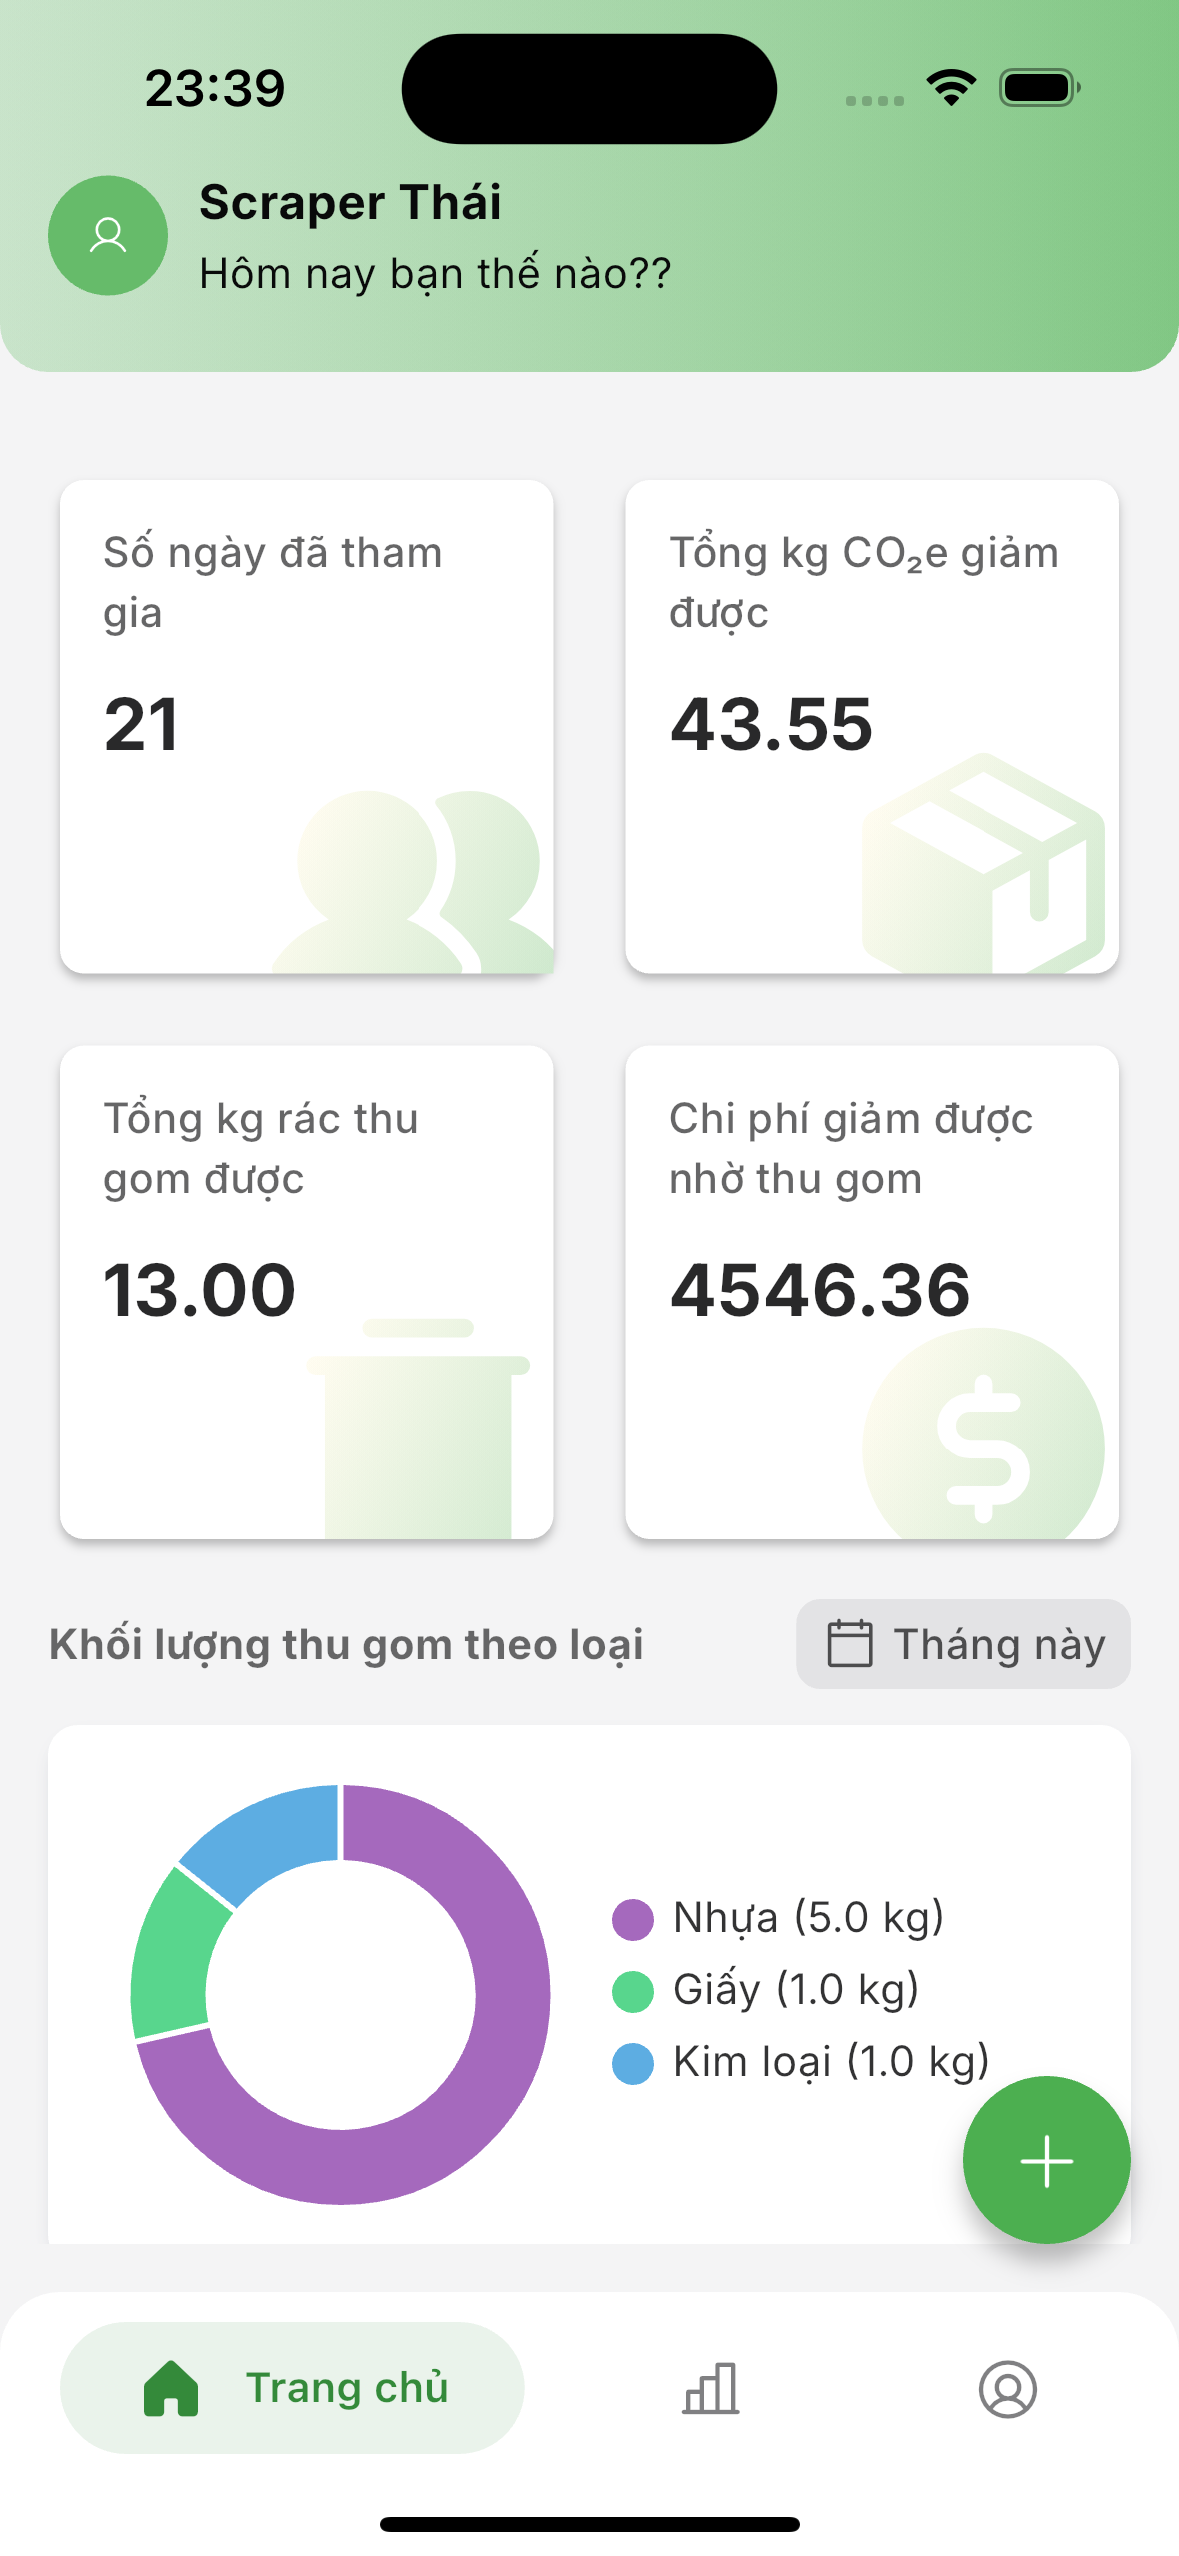
\includegraphics[width=0.32\textwidth]{Images/mobile/home_screen_scraper.png}}
  \hfill
  \subcaptionbox{Màn đóng góp dữ liệu}{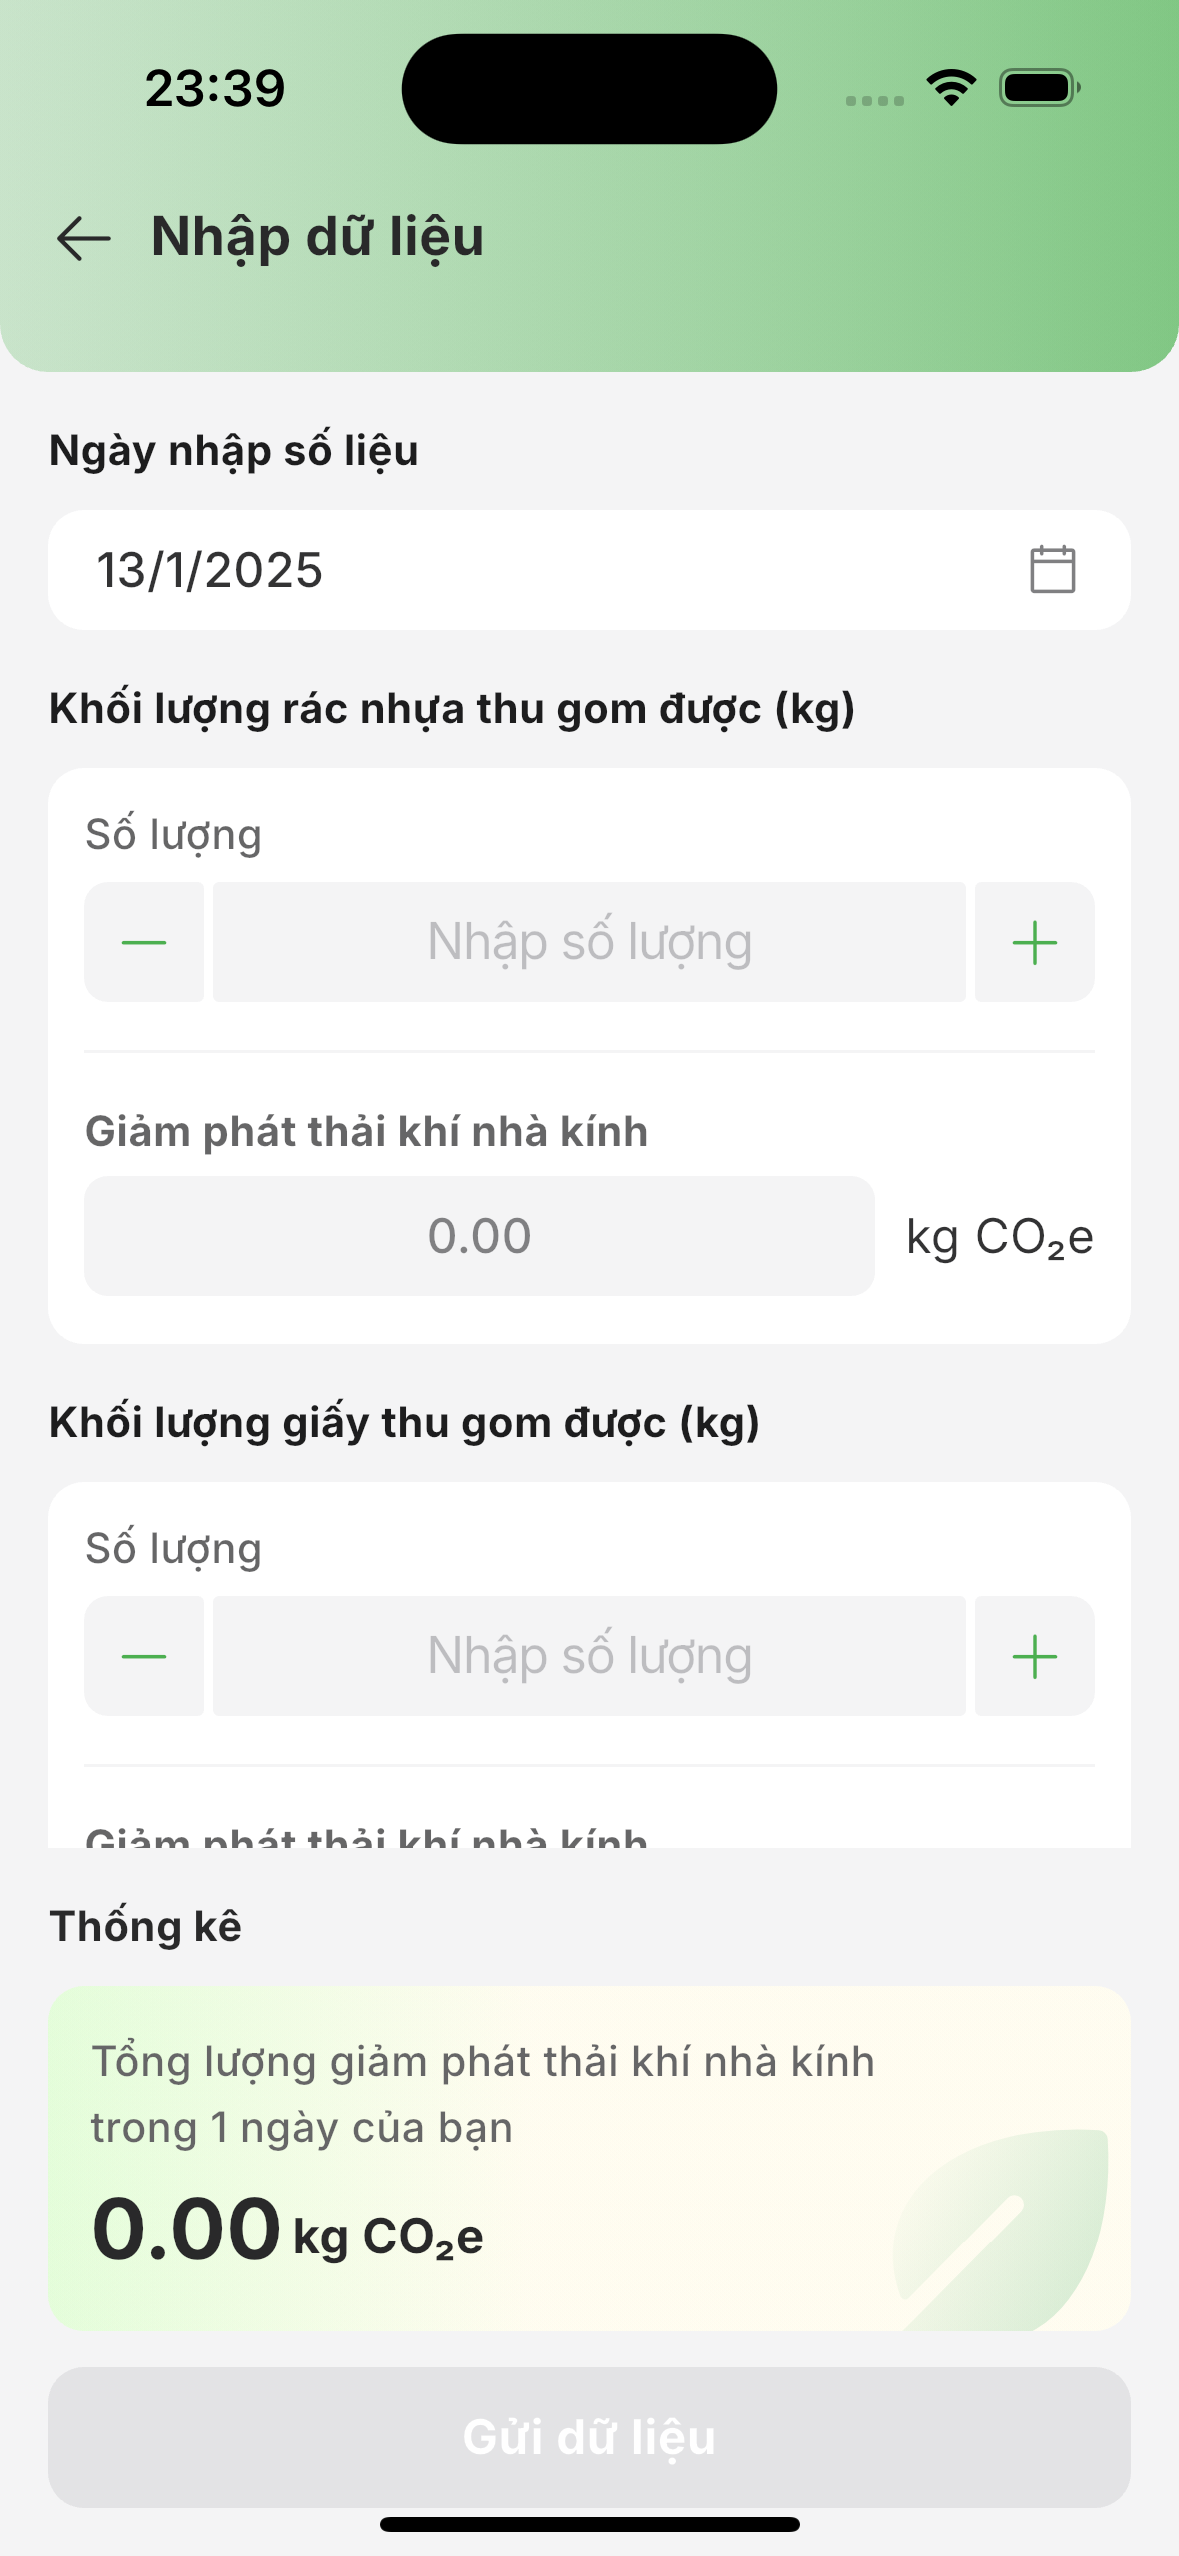
\includegraphics[width=0.32\textwidth]{Images/mobile/input_screen.png}}
  \hfill
  \subcaptionbox{Lượng giảm phát thải được tính toán}{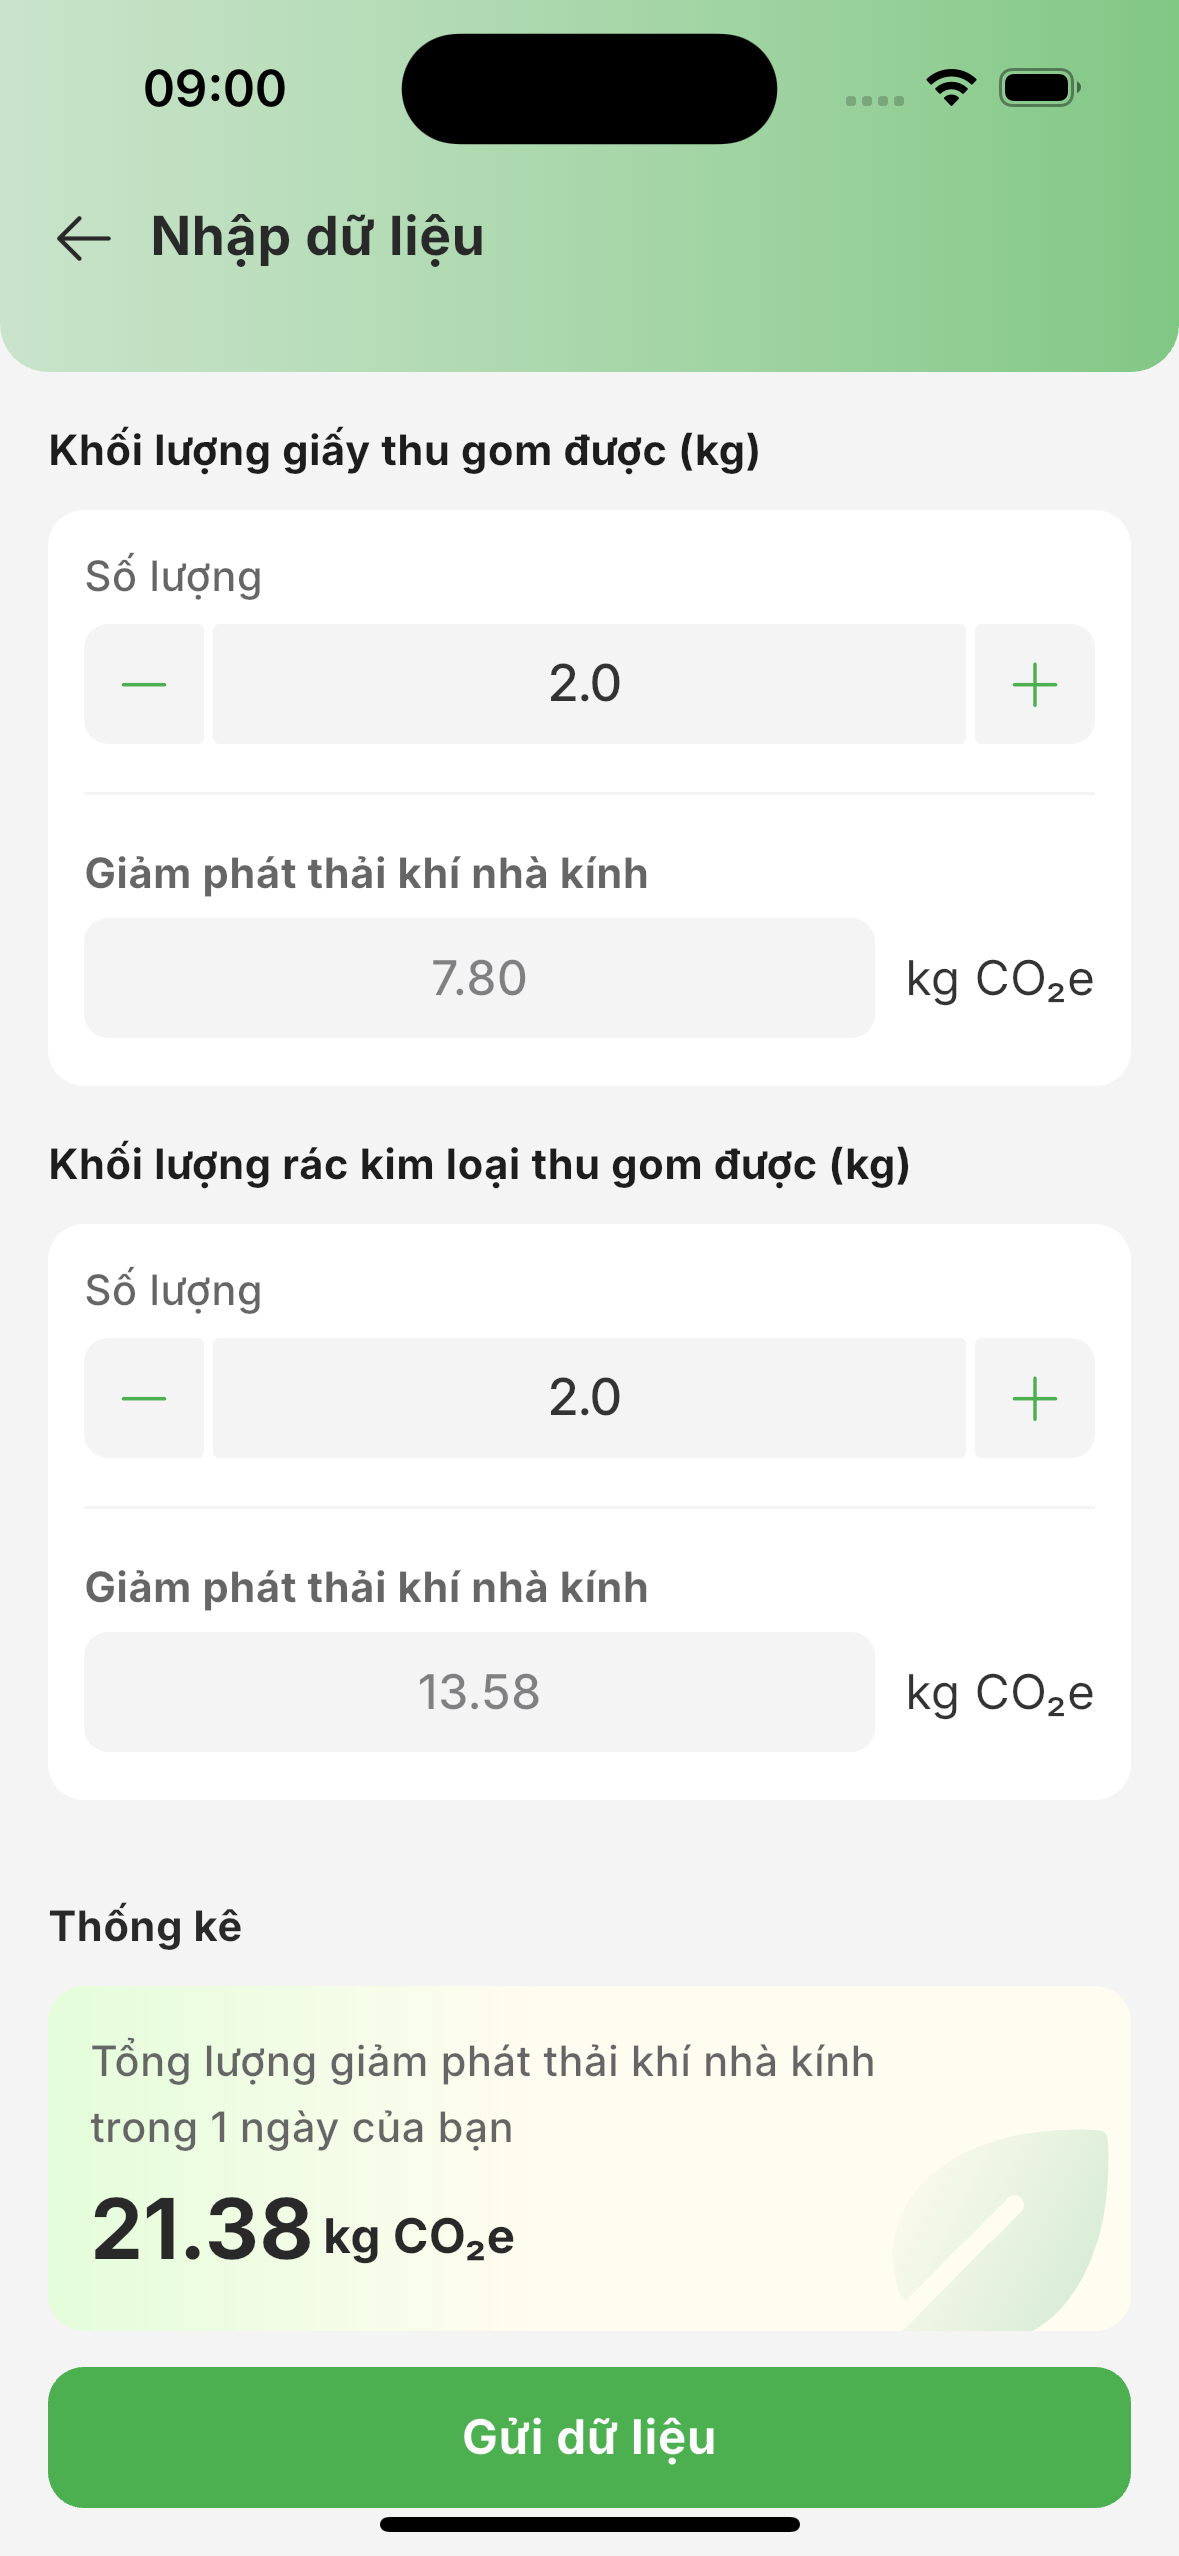
\includegraphics[width=0.32\textwidth]{Images/mobile/input_screen_with_value.png}}
  \caption[Hình ảnh màn chức năng nhập số liệu]{\bfseries \fontsize{12pt}{0pt}
  \selectfont Hình ảnh màn chức năng nhập số liệu}
  \label{input_statistic_waznet}
\end{figure}

\subsubsection{Chức năng đăng ký nhận thông báo nhập liệu hàng ngày}
Người dùng có thể nhận thông báo nhập số liệu hàng ngày theo khung giờ mong muốn, hệ thống sẽ gửi thông báo nhắc người dùng nhập số liệu \textbf{NẾU người dùng chưa nhập số liệu trong ngày đó}.

Các bước thực hiện bao gồm, nhấn vào tab \textbf{Tài khoản}, bật switch ở mục \textbf{Nhắc nhập liệu}, một khung thời gian hiện lên, người dùng thực hiện chọn thời gian và nhấn lưu để gửi lên hệ thống. Nếu người dùng muốn tắt thông báo, chỉ cần tắt switch. Hoặc nếu người dùng muốn đổi thời gian nhắc nhở, nhấn vào giờ trong mục \textbf{Nhắc nhập liệu} để thay đổi.

\begin{figure}[H]
  \centering
  \subcaptionbox{Chọn thời gian nhắc nhở}{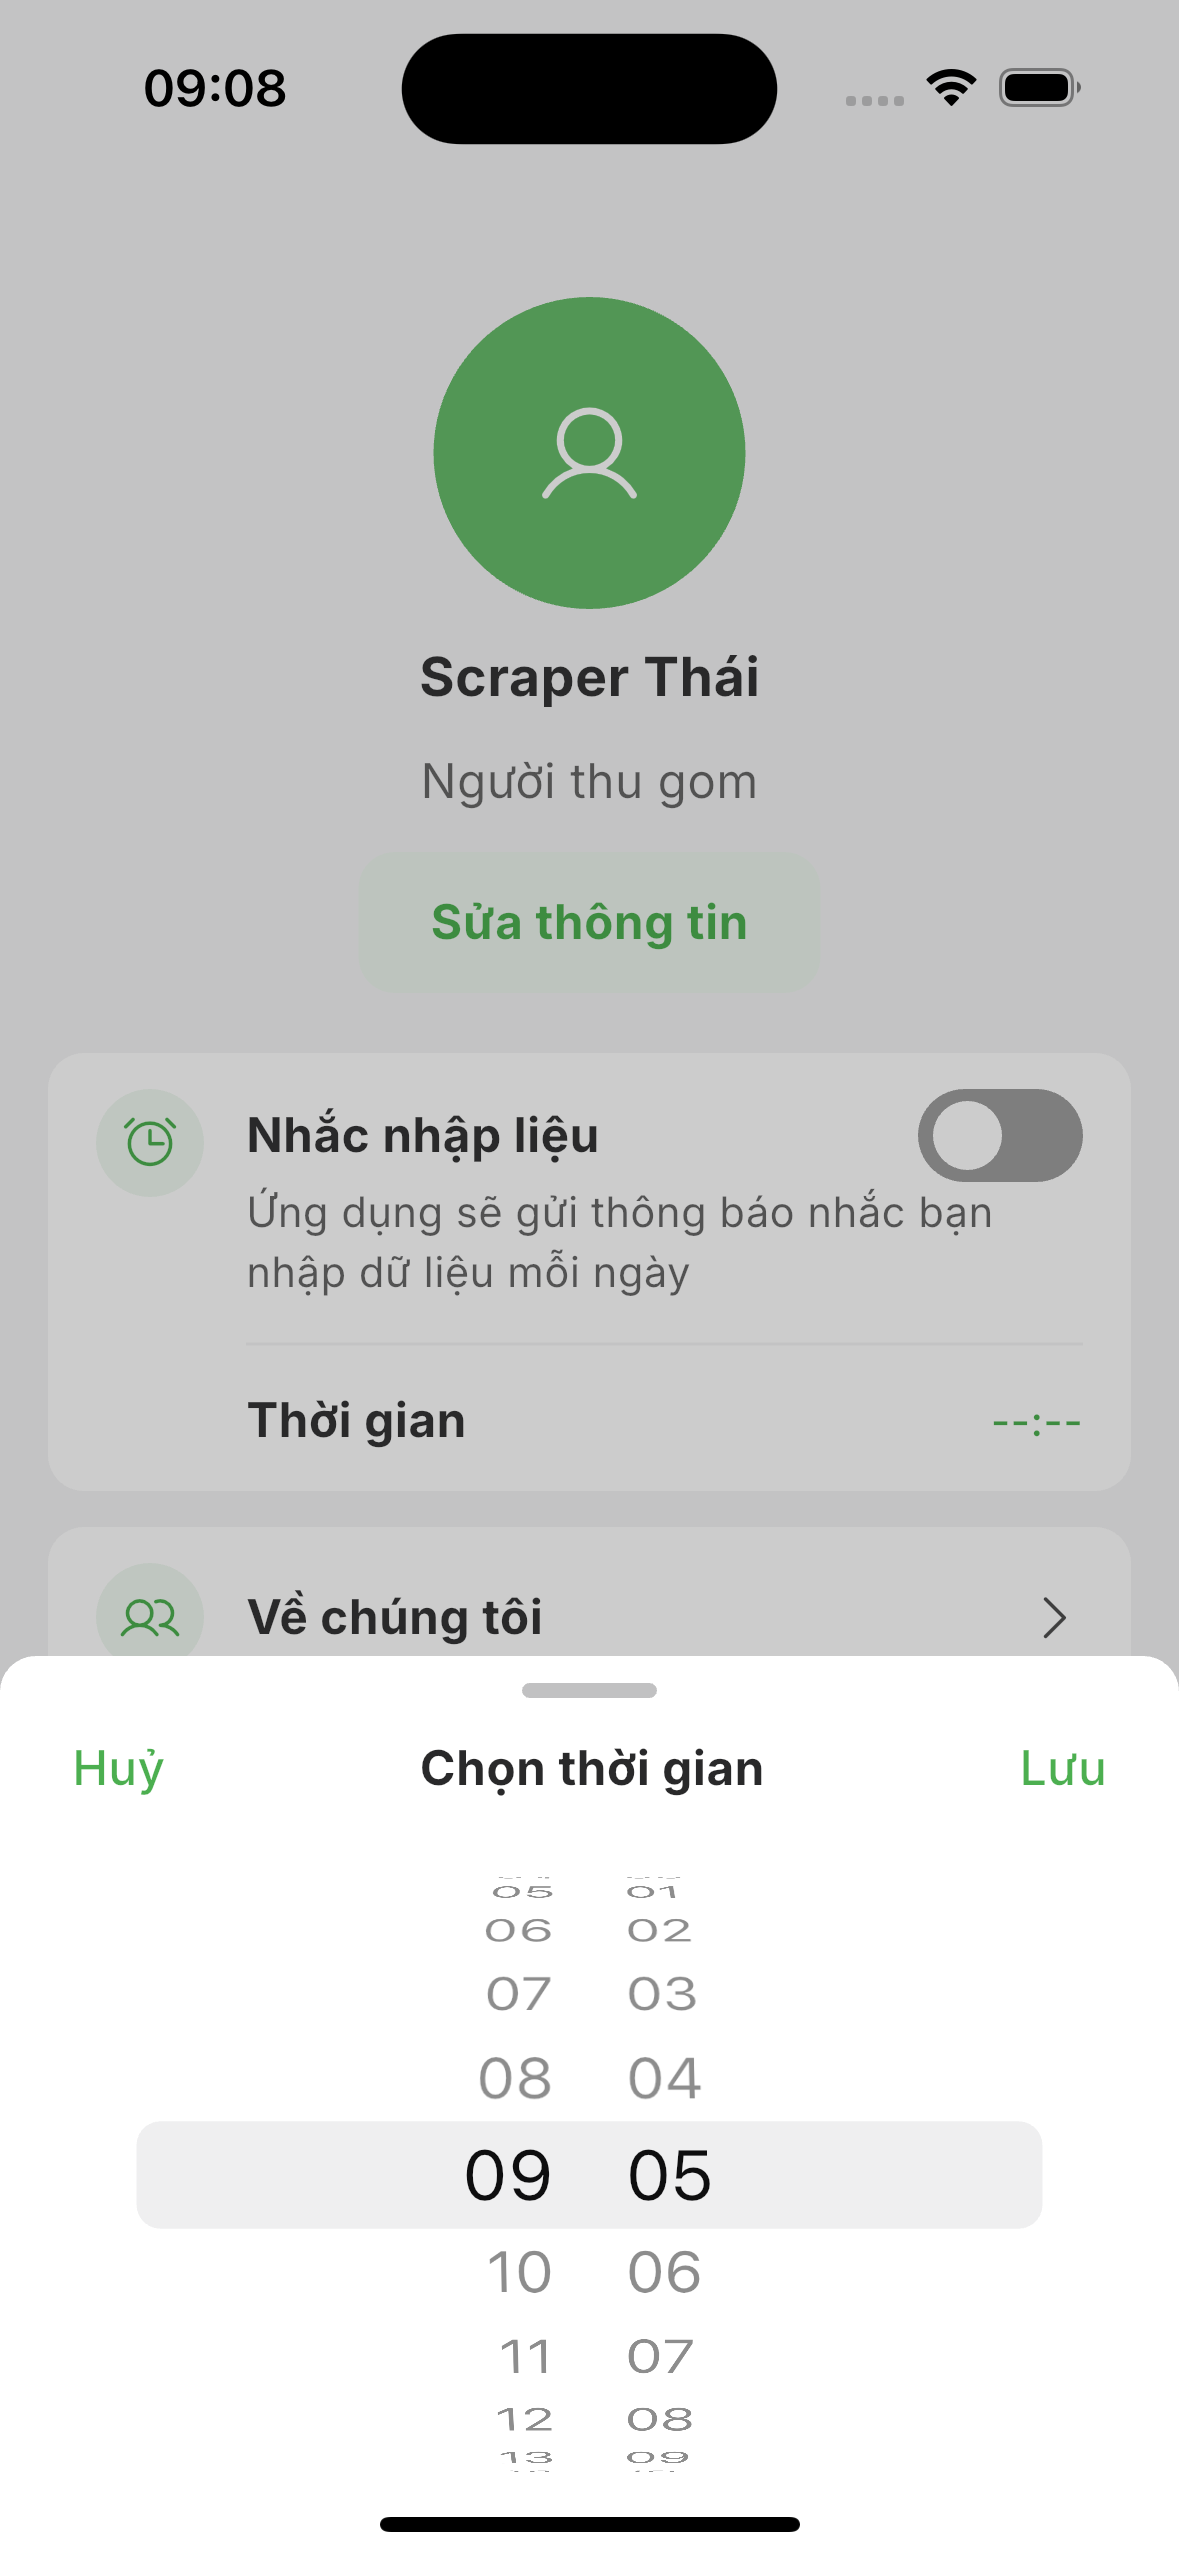
\includegraphics[width=0.45\textwidth]{Images/mobile/select_time_remind.png}}%
  \hfill
  \subcaptionbox{Thời gian nhắc nhở được chọn}{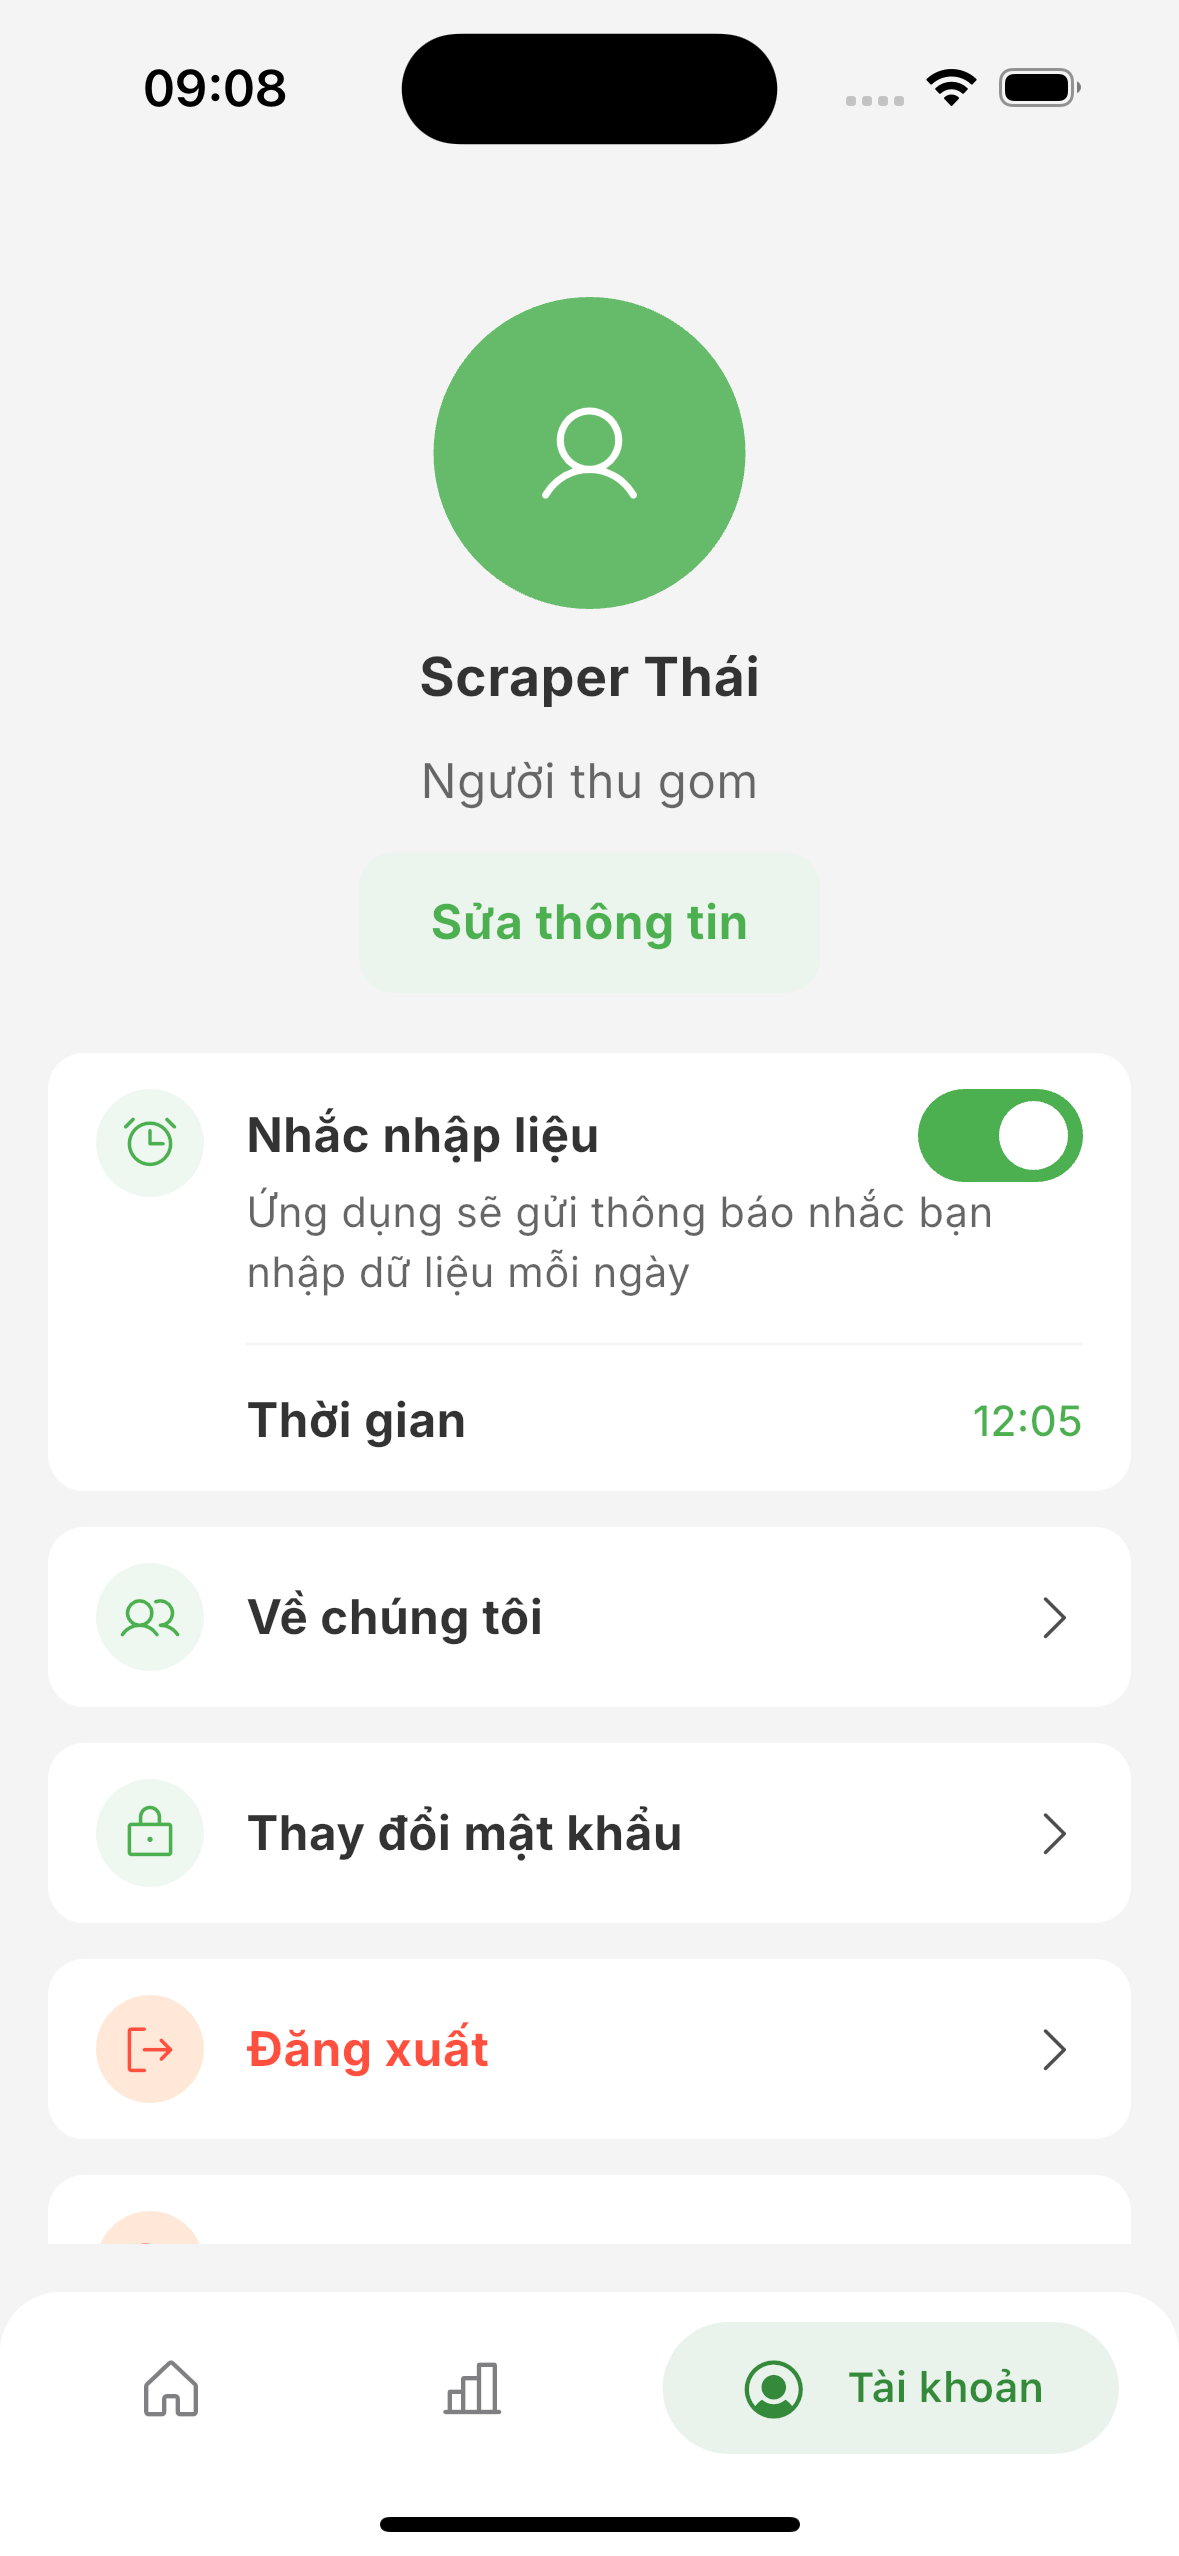
\includegraphics[width=0.45\textwidth]{Images/mobile/select_time_remind_2.png}}%
  \caption[Hình ảnh màn chức năng đăng ký nhận thông báo nhập liệu]{\bfseries \fontsize{12pt}{0pt}
  \selectfont Hình ảnh màn chức năng đăng ký nhận thông báo nhập liệu}
  \label{select_time_remind_waznet}
\end{figure}

\subsection{Các chức năng riêng cho Admin}
\subsubsection{Chức năng xuất excel theo khoảng thời gian}
Chức năng đang được bổ sung.
\newpage